\documentclass[small_title,unis]{book_class}
% \documentclass[small_title,section-equation]{book_class}
% \documentclass[big_title,section-equation,unis]{book_class}
% If big:
% \themaketitle{Course}{Title}{what}
% If small:
\thetitle{AGF-301 The Upper Polar Atmosphere\\Lecture Notes}
\lhead{{\footnotesize\textsc{\leftmark}}}

\pgfplotsset{compat=1.16}
\begin{document}
\maketitle
\tableofcontents

\chapter{Physics of space plasmas}
\begin{remark}
    Section made from lectures done by Jøran Moen. Other sources are \citet{1995Itsp} --- chapter 2.
\end{remark}

\section{Single particle motion}
\subsection{Gyro-motion}
We first look at the motion of single particles. From the equation of motion we have
\begin{equation*}
    m\frac{\text{d}\gf{v}}{\text{d}t}=q\gf{E}+\underbrace{q\gf{v}\times\gf{B}}_{\text{Lorentz}}+\cancelto{0}{m\gf{g}}
\end{equation*}
If we look at motion due to the magnetic field, the gyro-motion (cyclotron), we let \(\gf{E}=\gf{0}\), leaving only the magnetic field from the equation above, hence we get
\begin{equation*}
    m\frac{\text{d}{\gf{v}}}{\text{d}t}=q\gf{v}\times\gf{B}
\end{equation*}
\begin{align*}
    m\frac{\text{d}\gf{v}}{\text{d}t}&=q\gf{v}_\perp\times\gf{B}\\
    &=m\gf{a}_\perp=\frac{\gf{v}_\perp^2}{r_c}m\Rightarrow r_c=\frac{\gf{v}_\perp^2}{\gf{a}_\perp}=\frac{m\gf{v}_\perp}{q\gf{B}}
\end{align*}
So the only acceleration we have is the acceleration perpendicular to the magnetic field lines. The equation above describes gyro-motion, and the period of one gyration is
\begin{equation*}
    \tau_c=\frac{2\pi m}{qB}
\end{equation*}
with angular frequency
\begin{equation*}
    \omega_c=\frac{qB}{m}
\end{equation*}
\begin{figure}[t]
    \centering
    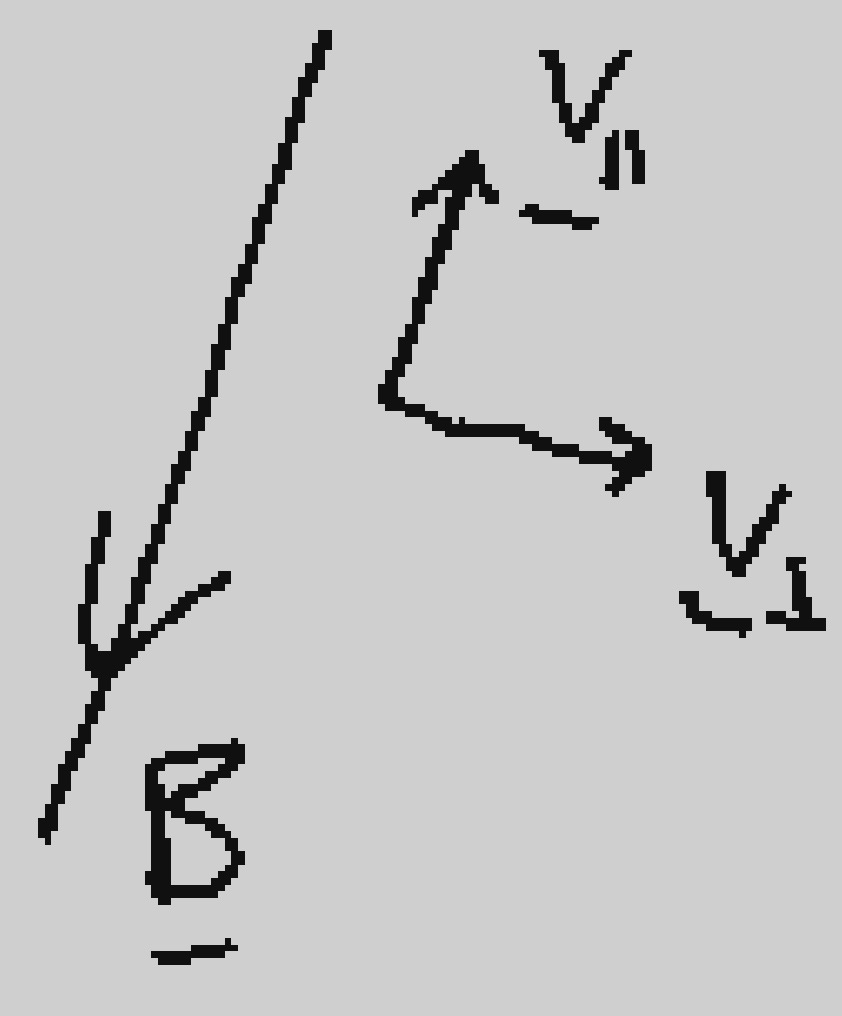
\includegraphics[width=.15\linewidth]{bilder/v_decomp.jpg}\label{fig:v_decomp}
    \caption{Graphical description of the definition of parallel and perpendicular directions.}
\end{figure}

\subsection{\(\gf{E}\times\gf{B}\)-drift}
We first want to look at the \(\orderof(0)\) of the motion of the single particles. We look at the parallel and perpendicular components individually. \boxed{\vert\vert:}
\begin{equation*}
    m\frac{\text{d}\gf{v}}{\text{d}t}=\gf{F}_{\vert\vert}=q\gf{a}_{\vert\vert}=0
\end{equation*}
\boxed{\perp:}
\begin{equation*}
    m\frac{\text{d}\gf{v}}{\text{d}t}=\gf{F}_\perp=q\gf{a}_\perp=0
\end{equation*}
\begin{figure}[t]
    \centering
    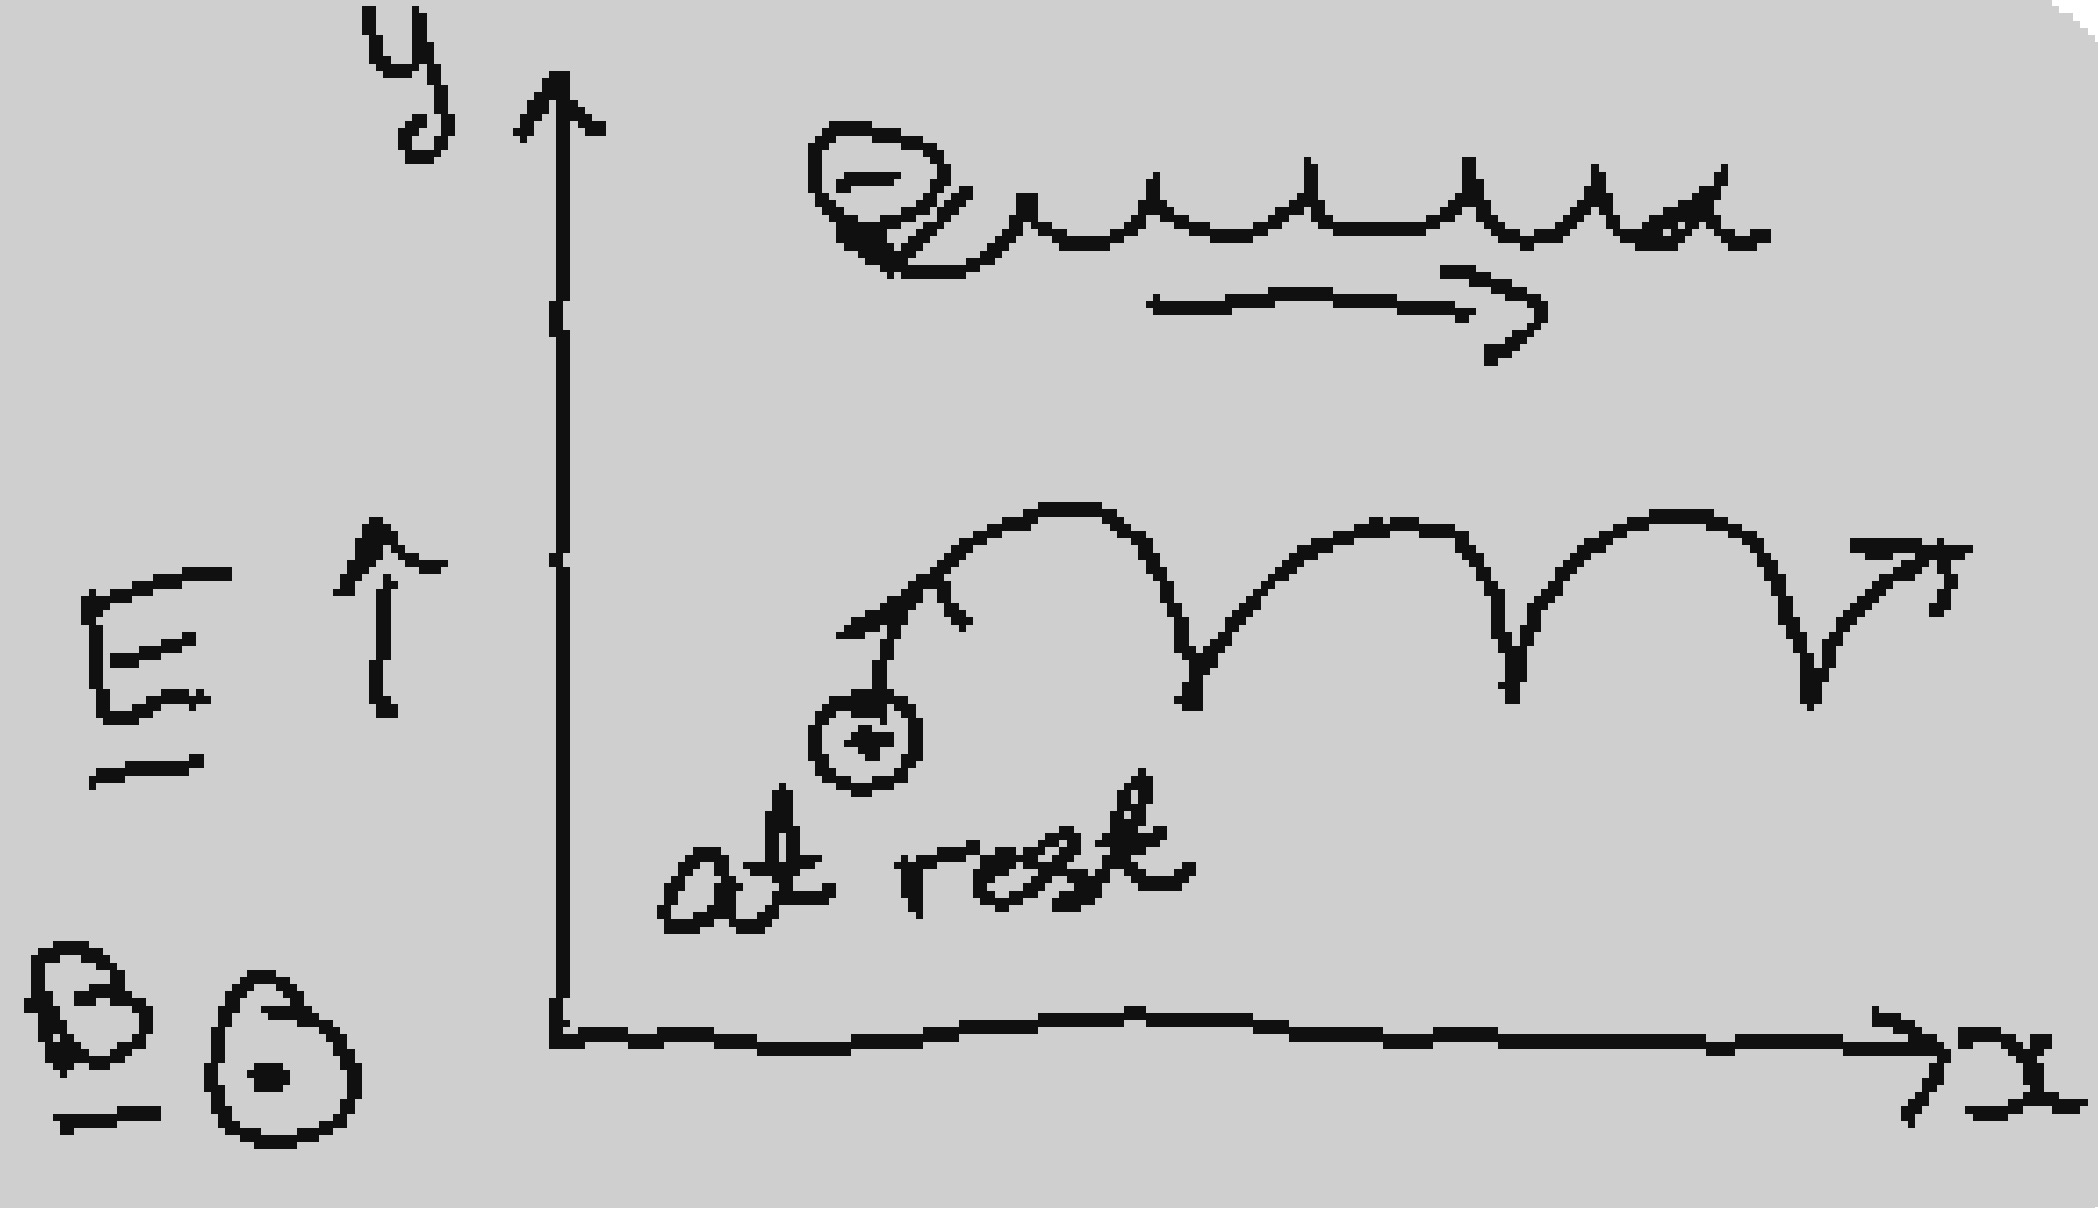
\includegraphics[width=0.2\linewidth]{bilder/ExB.jpg}\label{fig:ExB}
    \caption{\(\gf{E}\times\gf{B}\)-drift of ions and electrons.}
\end{figure}
We want to look at the drift we get from the \(E\)- and \(B\)-fields when they have perpendicular components. Let \(\gf{v}_\perp=\gf{u}_E+\gf{v}_\perp'\) where \(\gf{u}_E\) describe the constant motion and \(\gf{v}'\) describe accelerated motion.
\begin{align*}
    \Rightarrow m\frac{\text{d}\gf{v}'}{\text{d}t}+\cancelto{0}{m\fracdt{\gf{u}_E}}&=q\gf{E}_\perp+q\gf{v}'\times\gf{B}+q\gf{u}_E\times\gf{B}\\
    \underbrace{m\fracdt{\gf{v}'}-q\gf{v}'\times\gf{B}}_{\substack{=0 \textnormal{ when avg} \\\textnormal{over one period}}}&=q\gf{E}_\perp+q\gf{u}_E\times\gf{B}\quad\vert\times\gf{B}\\
    \gf{E}_\perp\times\gf{B}&=\gf{u}_{E}B^2-\gf{B}\cancelto{0}{(\gf{B}\cdot\gf{u}_E)}
\end{align*}
\begin{equation*}
    \therefore \gf{u}_E=\frac{\gf{E}\times\gf{B}}{B^2}
\end{equation*}
This generalizes to
\begin{equation}\label{eq:gen_v_drift}
    \gf{u}_F=\frac{\gf{F}\times\gf{B}}{qB^2}
\end{equation}

\subsection{\(\nabla\gf{B}\)-drift}
We linearize the magnetic parameter, i.e.\ we let \(\gf{B}=\gf{B}_0+(\partial_y\gf{B})y\f{z}+\orderof(2)\) where we assume the second order terms are negligible and where \(\gf{B}=B\f{z}\).
\begin{equation*}
    \gf{F}_x=qv_{y}B
\end{equation*}
\begin{align*}
    \gf{F}_y=-qv_{x}B&=m\dot{v}_y,\qquad\text{int.\ w.r.t } t\\
    mv_y=-qxB&=-qr_c\sin(\phi)B
\end{align*}
\coloredeqq{\Rightarrow{} v_y=-v_\perp\sin(\phi),\quad v_x=v_\perp\cos(\phi)}
To look at the average drift of the particle we simply average over one period
\begin{align*}
    \overline{\gf{F}_y}&=\frac{1}{2\pi}\int_0^{2\pi}-q\gf{v}_\perp\cos(\phi)\left[\gf{B}_0+{\left(\p{y}{\gf{B}}\right)}_\perp\gf{r}_c\cos(\phi)\right]\text{d}\phi \\
    &=\cancelto{0}{\int_0^{2\pi}-q\gf{v}_\perp\gf{B_0}\cos(\phi)\text{d}\phi}-\int_0^{2\pi}q\gf{v}_\perp\gf{r}_c\cos^2(\phi){\left(\p{y}{\gf{B}}\right)}_\perp\text{d}\phi \\
    &=-\frac{1}{2}q\gf{v}_\perp\gf{r}_c{\left(\p{y}{\gf{B}}\right)}_\perp \\
    &=-\frac{1}{2}\frac{mv_\perp^2}{B}{\left(\p{y}{\gf{B}}\right)}_\perp
\end{align*}
We may plug this into \cref{eq:gen_v_drift} to get the grad-B-drift velocity
\coloredeq{eq:grad_drift}{\gf{u}_{\nabla{} B}=\frac{1}{2}mv_\perp\frac{\gf{B}\times\nabla\gf{B}}{qB^3}}
\begin{figure}[t]
    \centering
    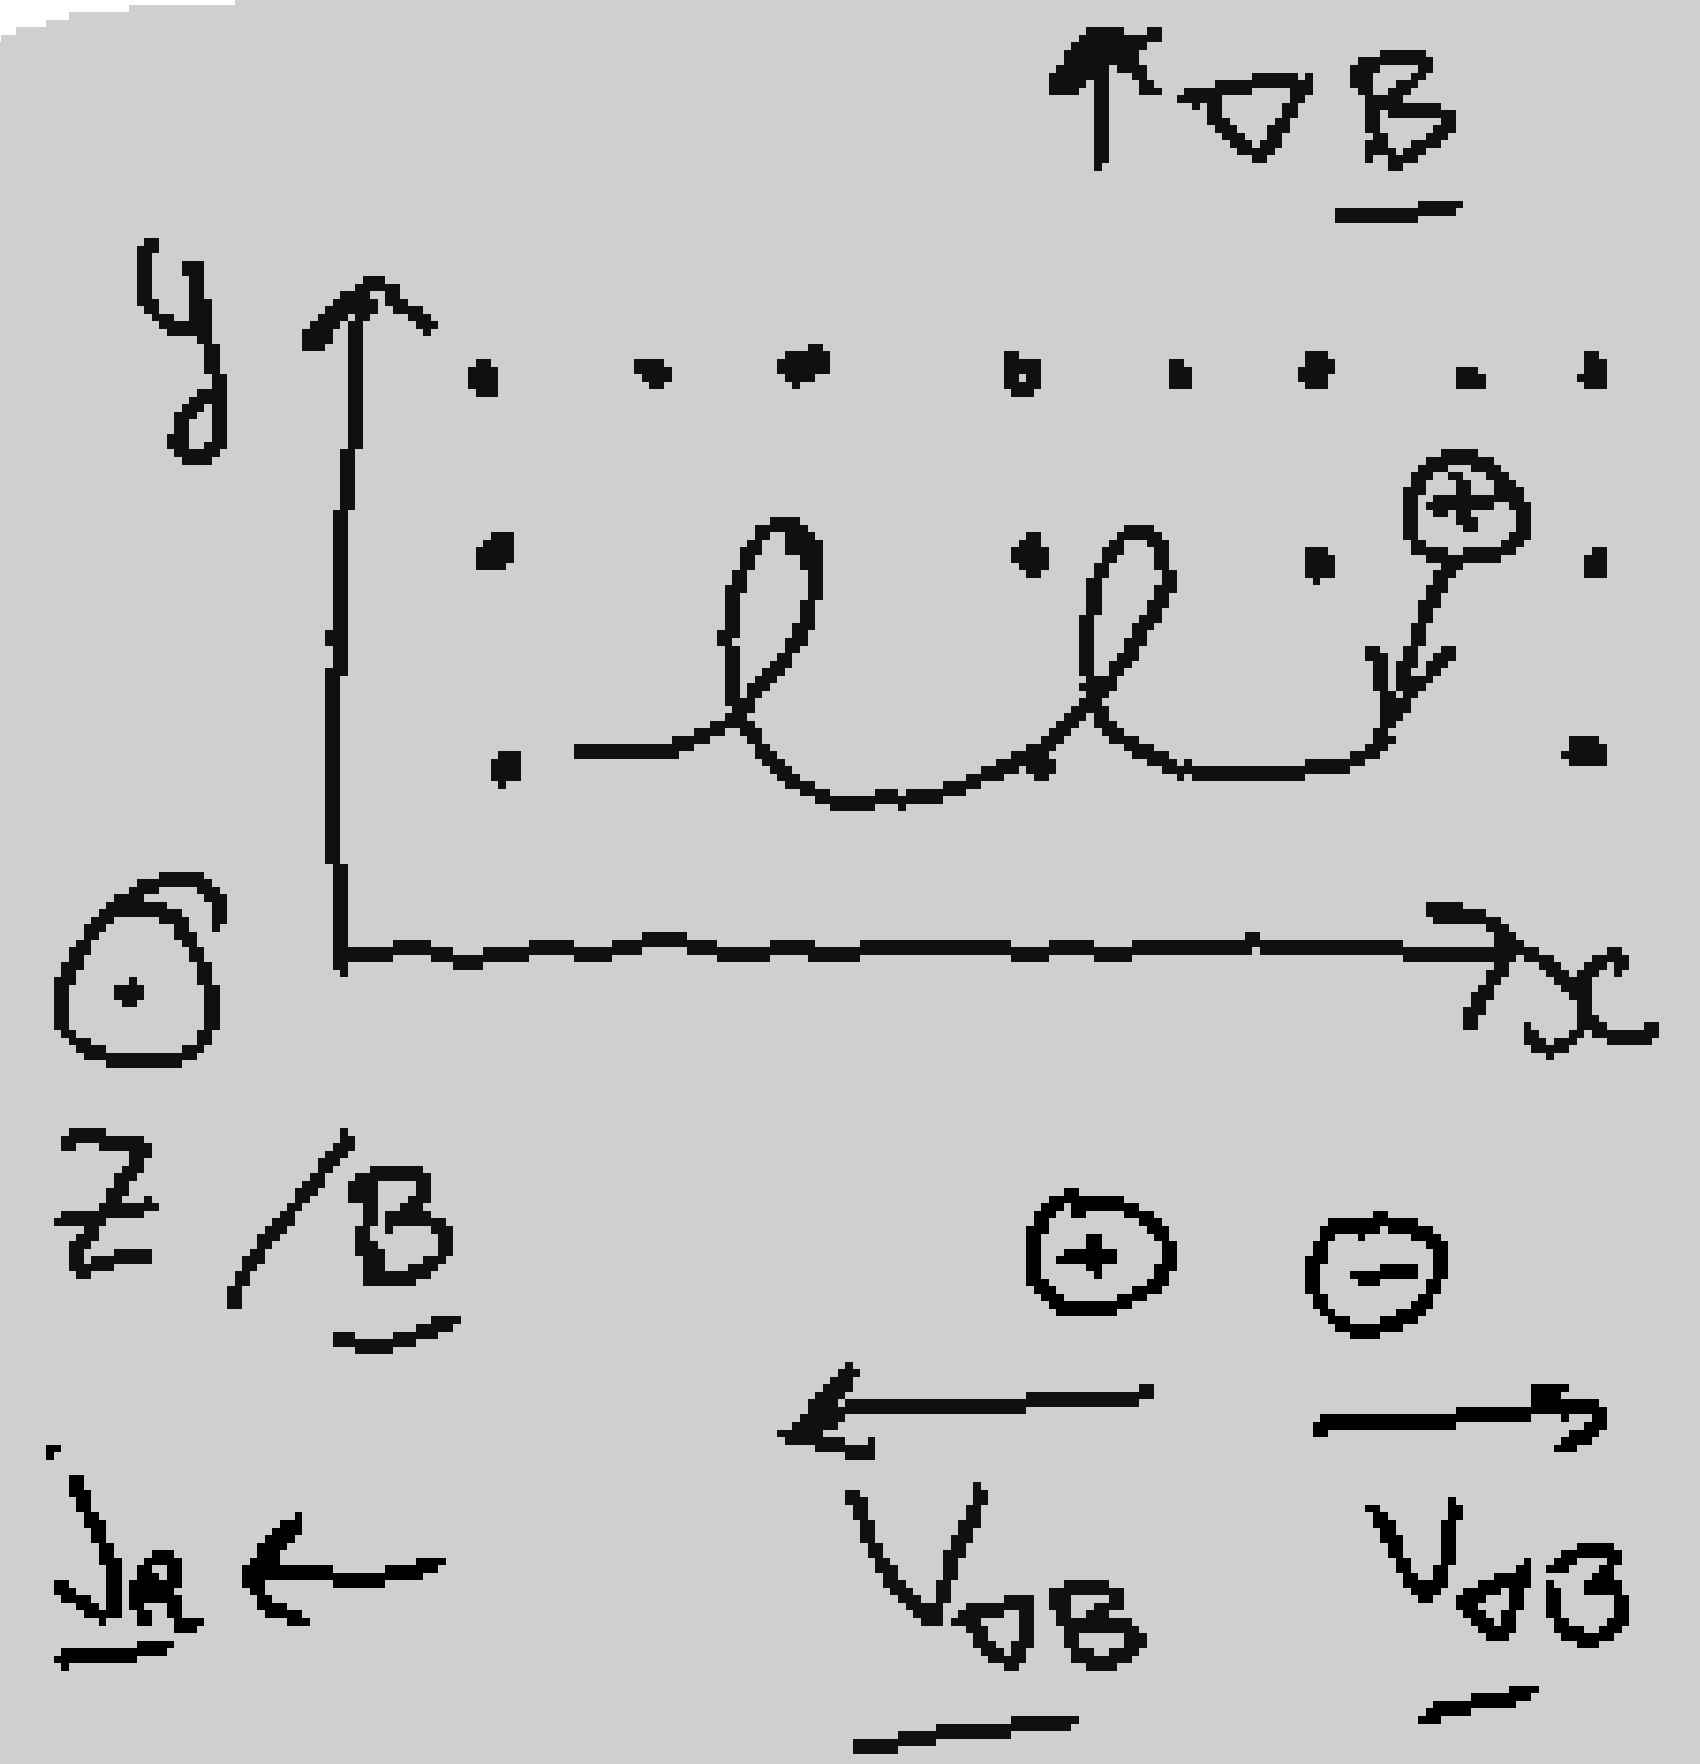
\includegraphics[width=0.2\linewidth]{bilder/gradB.jpg}\label{fig:gradB}
    \caption{\(\nabla\gf{B}\)-drift of ions and electrons.}
\end{figure}
This drift is dependant on charge, and from it we get a current, for instance \(\gf{j}_R~\sim \)~magnetic ring current. This is a current that runs in the westward direction.

\subsection{Curvature \(\gf{B}\)-drift}
A third drift we will look at is due to the curvature of the magnetic field lines, hence the name curvature \(B\)-drift. Let \(\gf{R}_c\) be the radius of a circle made up from the curving magnetic field lines. Motion parallel to these lines will then be described by
\begin{equation*}
    \gf{a}_{\vert\vert}=\frac{v^2_{\vert\vert}}{\gf{R_c}}
\end{equation*}
This give the centrifugal force
\begin{equation*}
    \gf{F}_{cf}=m\gf{a}_{\vert\vert}=m\frac{v^2_{\vert\vert}}{R_c^2}\gf{R}_c
\end{equation*}
This give the curvature drift when we plug this into \cref{eq:gen_v_drift} as
\coloredeq{eq:c_drift}{\gf{u}_{g}=m\frac{v^2_{\vert\vert}}{R_c^2}\frac{\gf{R}_c\times\gf{B}}{qB^2}}
Both \(\gf{u}_{\nabla B}\) and \(\gf{u}_{g}\) in \cref{eq:grad_drift,eq:c_drift} adds to the ring current.
\begin{figure}[t]
    \centering
    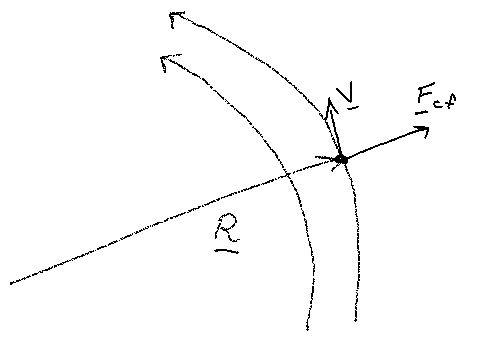
\includegraphics[width=.4\linewidth]{bilder/curve_drift.png}\label{fig:curve_drift}
    \caption{Curvature drift}
\end{figure}
\begin{figure}[t]
    \centering
    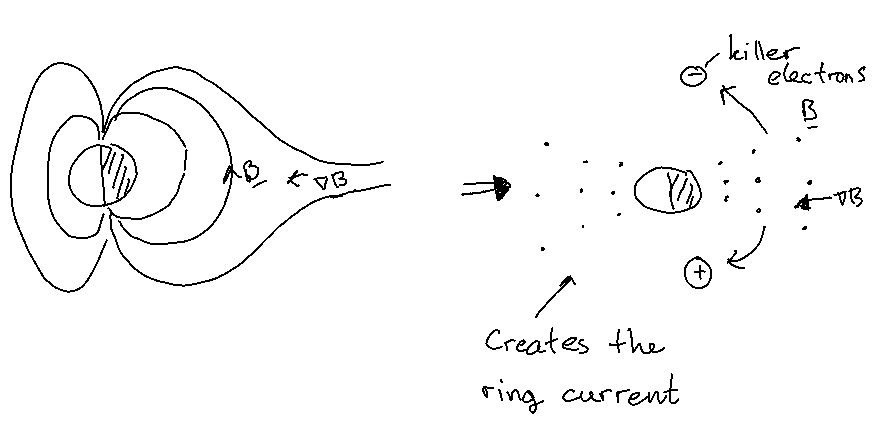
\includegraphics[width=.6\linewidth]{bilder/ring_current.png}\label{fig:ring_current}
    \caption{Ring current}
\end{figure}

\subsection{Magnetic momentum}
The magnetic moment is a quantity that will stay constant even though the energy changes, if the field changes slowly enough. Slowly enough means that the field changes encountered by the particle within a single gyration orbit will be small compared with the initial field. The magnetic moment is defined as \(\mu=IA\) where \(I=\Delta Q/\Delta t=q\omega_c/2\pi=q^2B/2\pi m\) is the current and \(A=\pi r_c^2=\pi mv_\perp/qB\) is the area spanned out by the gyro motion. Plugging the current and the area into the expression for magnetic momentum gives
\coloredeq{eq:magnetic_moment}{\mu=\frac{1}{2}\frac{mv_\perp^2}{B}}
This is known as the \emph{first magnetic invariant}. If we look at the magnetic moment at some point \(E\) along a magnetic field line, we may write the perpendicular component of the velocity in terms of a sine function with argument \(\alpha \), where \(\alpha \) is the angle off the magnetic field line.
\begin{align}
    \mu_E&=\frac{1}{2}\frac{mv_\perp^2}{B_E}\notag \\
    &=\frac{1}{2}\frac{mv^2}{B_E}\sin^2\alpha
\end{align}
\begin{align}
    \mu_M&=\frac{1}{2}\frac{mv_\perp^2}{B_M}\notag \\
    &=\frac{1}{2}\frac{mv^2}{B_M}
\end{align}
where the subscript \(M\) defines the mirror point where we only have a perpendicular velocity component. Since the magnetic moment is conserved we can compare these two to obtain
\begin{align*}
    \mu_E&=\mu_M\\
    \frac{1}{2}\frac{mv^2}{B_E}\sin^2\alpha&=\frac{1}{2}\frac{mv^2}{B_M}
\end{align*}
\begin{equation}
    B_M=\frac{B_E}{\sin^2\alpha}
\end{equation}
and we see how the strength of the magnetic field varies due to them converging when you move closer to the pole. If the angle at point \(E\) is such that \(B_M\) can never get big enough, the particle is lost down to the atmosphere, from which we can define a loss cone as illustrated in \cref{fig:loss_cone}.
\begin{figure}[t]
    \centering
    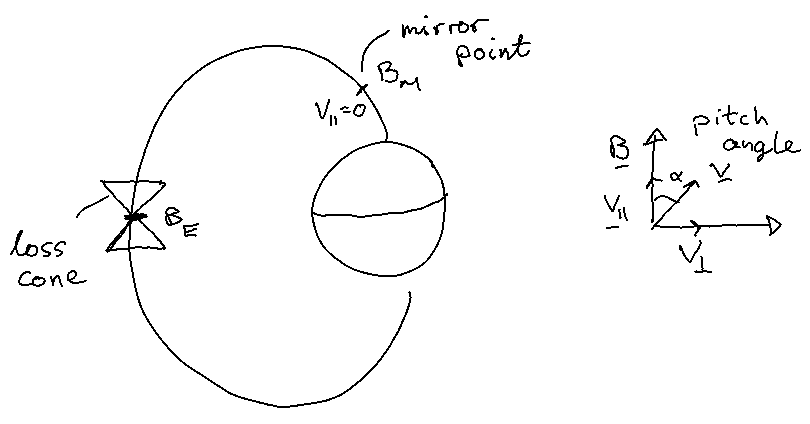
\includegraphics[width=.6\linewidth]{bilder/loss_cone.png}
    \caption{Loss cone}\label{fig:loss_cone}
\end{figure}

\section{Collection of particles}
We will now move on from just describing the motion on one single particle by considering collections of particles. It is handy to introduce the phase space function \(f(\gf{r},\gf{v},t)\)
\begin{align*}
    \gf{r}&=(x,y,z)\\
    \gf{v}&=(v_x,v_y,v_z)\\
    \text{d}\gf{v}\text{d}\gf{r}&=\text{d}v_x\text{d}v_y\text{d}v_z\text{d}x\text{d}y\text{d}z
\end{align*}
From this function you can get information from looking at the different orders of momentum. The \emph{zeroth order momentum} give the number density
\begin{equation*}
    n(\gf{r},t)=\int_{-\infty}^\infty f(\gf{r},\gf{v},t)\text{d}\gf{v}
\end{equation*}
which is related to the mass density \(\rho=nm_i\). The \emph{first order momentum} will give the average velocity of your distribution
\begin{equation*}
    \gf{u}(\gf{r},t)=\overline{\gf{v}(\gf{r},t)}=\frac{\int_{-\infty}^\infty vf(\gf{r},\gf{v},t)\text{d}\gf{v}}{\int_{-\infty}^\infty f(\gf{r},\gf{v},t)\text{d}\gf{v}}
\end{equation*}
while the \emph{second order momentum} give the average energy
\begin{equation*}
    E=\frac{1}{2}m\overline{\gf{v}^2(\gf{r},t)}=\frac{\int_{-\infty}^\infty v^2f(\gf{r},\gf{v},t)\text{d}\gf{v}}{\int_{-\infty}^\infty f(\gf{r},\gf{v},t)\text{d}\gf{v}}
\end{equation*}

\subsection{Maxwellian distribution}
For a uniform, isotropic, and stationary system/plasma, the phase space distribution function reduces to a function of velocity only, often described by a Maxwellian distribution.
\begin{equation*}
    f(v_x)=Ae^{-\frac{1}{2}m{(v_x-u_x)}^2/kT}
\end{equation*}
where \(A\) is the normalization constant. The number density will be
\begin{align*}
    n_s&=A\int_{-\infty}^\infty e^{-\frac{1}{2}m{(v_x-u_x)}^2/kT}\text{d}v_x,\quad a=\sqrt{\frac{m}{2kT}}(v_x-u_x),\text{d}a=\sqrt{\frac{m}{2kT}}\text{d}v_x\\
    &=A\sqrt{\frac{2kT}{m}}\int_{-\infty}^\infty e^{-a^2}\text{d}a\\
    &=A\sqrt{\frac{2kT}{m}}\sqrt{\pi}
\end{align*}
\begin{equation*}
    \therefore A=n\sqrt{\frac{m}{2\pi kT}}
\end{equation*}

\begin{txboxed}
\textbf{ASIDE:} If we look at a point from different places, say Longyearbyen and Tromsø, we may write up the phase space function with the velocity decomposed. We get the bi-Maxwellian distribution
\begin{equation*}
    f(r,t)=A'\exp\left[-\frac{1}{2}\frac{m{(v_{\vert\vert}-u_{\vert\vert})}^2}{kT_{\vert\vert}}\right]\exp\left[-\frac{1}{2}\frac{m{(v_{\perp}-u_{\perp})}^2}{kT_\perp}\right]
\end{equation*}
\end{txboxed}


\section{Fluid description of plasmas}
\subsection{Magneto-Hydro Dynamics}
We look at a mixture of electrons and ions. We assume we have quasi-neutrality, i.e.\ that \(n_e\approx n_i\approx n\).
\begin{align*}
    \rho&=n(m_i+m_e)\\
    \gf{v}&=\frac{1}{\rho}(n_{i}m_i\gf{v}_i+n_{e}m_e\gf{v}_e)=\frac{n}{\rho}(m_i\gf{v}_i+m_e\gf{v}_e)\\
    \gf{j}&=ne(\gf{v}_i-\gf{v}_e)
\end{align*}
We want to derive the momentum equation for our plasma, so we first use the momentum equation for ions
\begin{equation*}
    \p{t}{(nm_i\gf{v}_i)}=en(\gf{E}+\gf{v}_i\times\gf{B})-\nabla p_i+m_{i}n\gf{g}+\gf{P}_{ie}
\end{equation*}
where \(p=nkT\) and \(\gf{P}_{ie}\propto nm_i\nu_{ie}(\gf{v}_i-\gf{v}_e)\) is the Coulomb collision term, the momentum transfer from the electrons to the ions and \(\nu_{ie}\) is the collision frequency. Then we look at the momentum equation for electrons
\begin{equation*}
    \p{t}{(nm_e\gf{v}_e)}=-en(\gf{E}+\gf{v}_e\times\gf{B})-\nabla p_e+m_{e}n\gf{g}+\gf{P}_{ei}
\end{equation*}
We then add the two to obtain one of the MHD equations
\begin{equation*}
    \p{t}{\left[n\left(m_i\gf{v}+m_e\gf{v}_e\right)\right]}=en(\gf{v}_i-\gf{v}_e)\times\gf{B}-\nabla\left(p_i+p_e\right)+n(m_i+m_e)\gf{g}
\end{equation*}
\coloredeq{eq:MHD}{\p{t}{\left(\rho\gf{v}\right)}&=\gf{j}\times\gf{B}-\nabla{} p+\rho\gf{g}}
If \(T_i=T_e\) we can find from \(p_i=nkT_i\) and \(p_e=nkT_e\) that \(p=2nkT\).
Other MHD equations are
\begin{align}
    \p{t}{\rho}+\nabla\cdot\left(\rho \gf{v}\right)&=0\label{eq:MHD_1}\\
    \rho\left[\p{t}{\gf{v}}+(\gf{v}\cdot\nabla)\gf{v}\right]&=-\nabla p+\gf{j}\times\gf{B}\label{eq:MHD_2}\\
    \nabla\times\gf{E}&=-\p{t}{\gf{B}}\label{eq:MHD_3}\\
    \nabla\times\gf{B}&=\mu_0\gf{j}\label{eq:MHD_4}\\
    \gf{j}&=\sigma(\gf{E}+\gf{v}\times\gf{B})\label{eq:MHD_5}\\
    p\rho^{-1}&=\text{const},\quad \tn{adiabatic transformation}\label{eq:MHD_6}
\end{align}
We want to find the \emph{Reynold number}. We then use \cref{eq:MHD_4,eq:MHD_5} and find the curl of this to obtain
\begin{align*}
    \nabla\times\left(\nabla\times\gf{B}\right)&=\nabla\times\mu_0\gf{j}=\nabla\times\left[\mu_0\sigma(\gf{E}+\gf{v}\times\gf{B})\right]\\
    &=\mu_0\sigma\left(-\p{t}{\gf{B}}+\nabla\times\left[\gf{v}\times\gf{B}\right]\right)
\end{align*}
We then rewrite this so that the local time derivative of the magnetic field is on the LHS, and we use one of the vector identities to rewrite the term on the left
\begin{equation*}
    \p{t}{\gf{B}}=\underbrace{\nabla\left(\gf{v}\times\gf{B}\right)}_{\substack{\tn{convection}\\ \tn{term}}}+\underbrace{\frac{1}{\mu_0\sigma}\nabla^2\gf{B}}_{\substack{\tn{diffusion}\\ \tn{term}}}
\end{equation*}
We define the Reynold number to be
\begin{align*}
    R_m&=\frac{\tn{convection term}}{\tn{diffusion term}}=\frac{\nabla\left(\gf{v}\times\gf{B}\right)}{\frac{1}{\mu_0\sigma}\nabla^2\gf{B}}\\
    &=\frac{\frac{1}{L}vB}{\frac{1}{\mu_0\sigma}\frac{1}{L^2}B}=L\mu_0\sigma v
\end{align*}
where we have used that the gradient scales as \(\nabla\sim 1/L\). If \(R_m\gg 1\) then MHD is applicable, otherwise it is not.


\chapter{Earth's geomagnetic field}
\begin{remark}
    Section made from lectures done by Dr.\ Emma Bland. Other sources are \citet{BrekkeAsgeir2013Potu} --- chapter 3 part 1 to 7, chapter 6.5 and chapter 7.1 --- and \citet{TwymanR.M.GEAS}.
\end{remark}

\section{Sources to the Earth's magnetic field}
Sources to the magnetic field of the Earth are (1) the core/main field (\cref{fig:L3_contributor1,fig:L3_contributor2}). This come from a self-sustaining dynamo action in the Earth's outer liquid core and contributes to more than 95\% of total field strength. The field strength is \(\approx\SI{25}{\micro\tesla}\) at equator and \(\approx\SI{65}{\micro\tesla}\) at the poles and the field can be described by a simple dipole model, with axis tilted \(\sim\SI{11}{\degree}\) from Earth’s rotation axis. This model have an error of \(\sim 30\% \) for \(R<4R_E\), while closer to the Earth the error is within \(10\% \). Another source is the (2) crustal field (\cref{fig:L3_contributor3}). This come from ferromagnetic minerals in the Earth’s crust and the contribution is typically a few hundred \si{\nano\tesla}, but up to thousands of \si{\nano\tesla} at some locations (can affect compasses). The (3) external field (\cref{fig:L3_contributor3}) is a third contribution. This arises from electric currents flowing in ionosphere and magnetosphere. Under quiet conditions it gives only fractions of \si{\nano\tesla} while a large geomagnetic storm can give thousands of \si{\nano\tesla}. Finally a fourth source is (4) electromagnetically induced fields (\cref{fig:L3_contributor3}). This is generated by currents induced in the crust and upper mantle by temporal fluctuations in the external field and gives up to tens of \si{\nano\tesla}.
\begin{figure}[ht]
	\centering

    \begin{subfigure}[t]{0.3\textwidth}
        \centering
        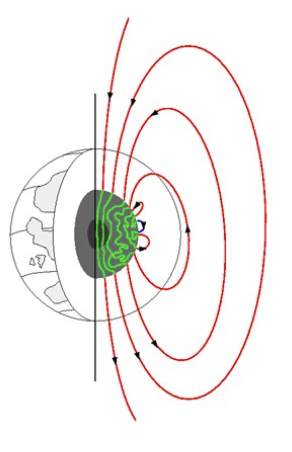
\includegraphics[width=.9\linewidth]{bilder/L3_earth_four_1.png}
        \caption{}\label{fig:L3_contributor1}
    \end{subfigure}
	\begin{subfigure}[t]{0.3\textwidth}
		\centering
		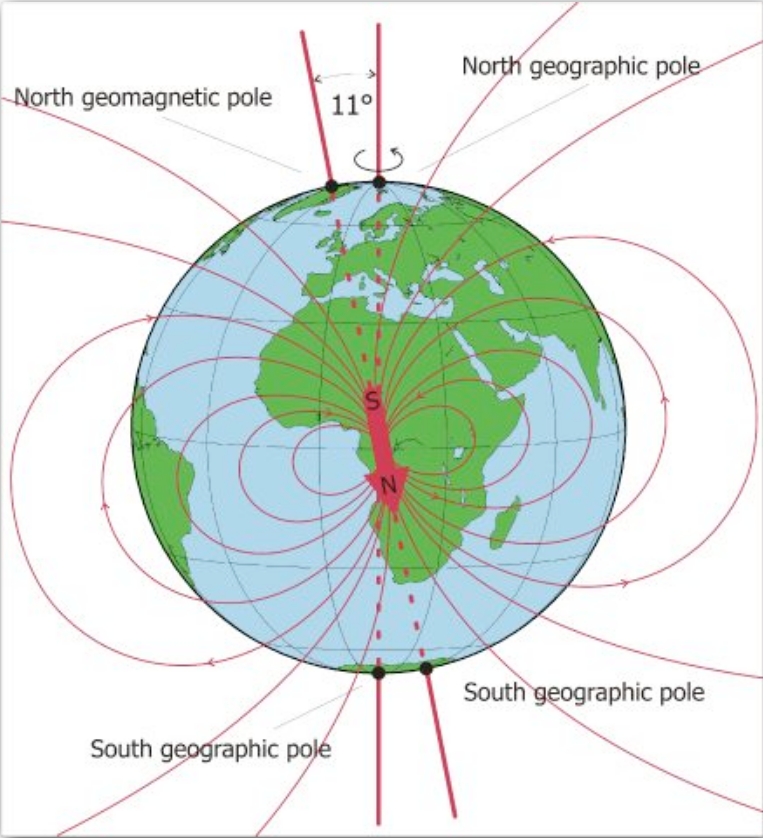
\includegraphics[width=.9\linewidth]{bilder/L3_earth_four_2.png}
		\caption{}\label{fig:L3_contributor2}
    \end{subfigure}
    \begin{subfigure}[t]{0.3\textwidth}
		\centering
		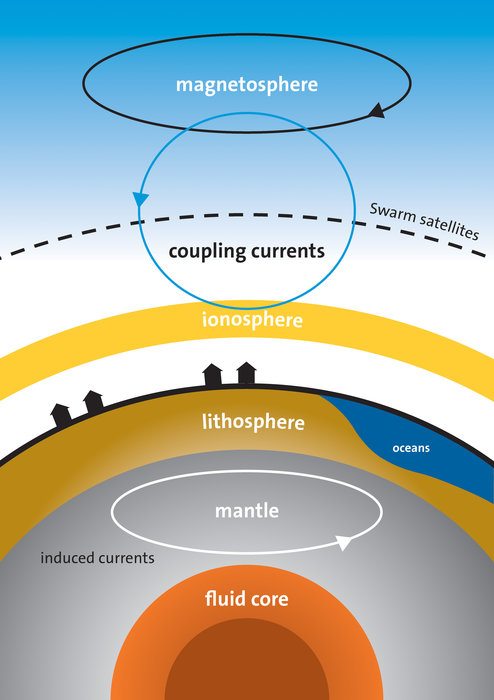
\includegraphics[width=.9\linewidth]{bilder/L3_earth_four_3.jpg}
		\caption{}\label{fig:L3_contributor3}
	\end{subfigure}

	\caption{The different contributors to the magnetic field.}\label{fig:L3_earth_magnetic_four_contributors}
\end{figure}
\begin{figure}[ht]
    \centering
    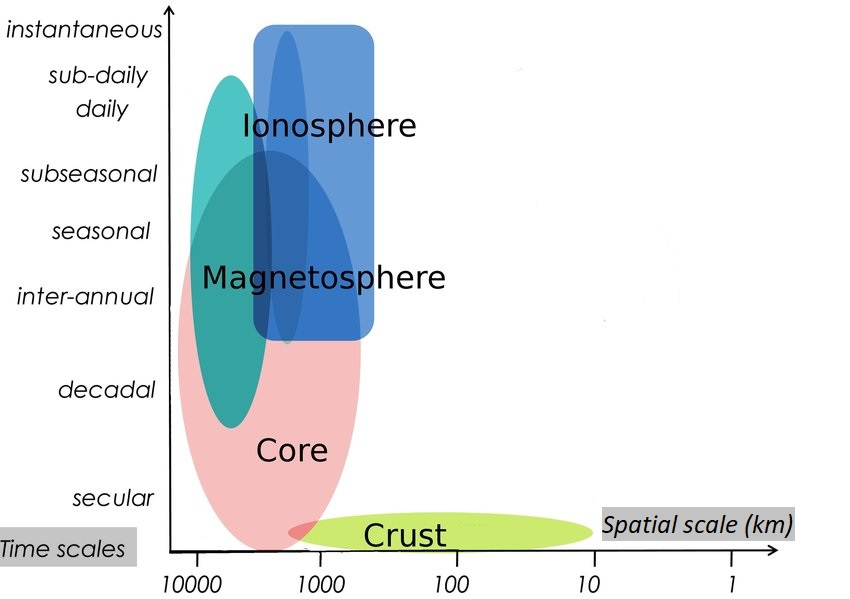
\includegraphics[width=.6\linewidth]{bilder/L3_earth_magnetic_contributors.jpg}\label{fig:L3_earth_magnetic_contributors}
    \caption{Spatial and temporal variations in the Earth's magnetic field. Source: }
\end{figure}

\section{Magnetic field in equation form}
We neglect currents flowing between Earth's surface and space. Outside the Earth:
\begin{equation*}
    \gf{j}=0\quad\Rightarrow\quad\nabla\times\gf{B}=0
\end{equation*}
where we have used \cref{eq:MHD_5}. We must then have a magnetic potential \(\Phi_m\) such that \(\gf{B}=-\nabla\Phi_m\). Also \(\nabla\cdot\gf{B}=0~~\therefore \nabla^2\Phi_m=0\).

We will now write the components of \(\gf{B}\) in spherical coordinates, as
\begin{equation}
    \nabla\Phi_m=\p{r}{\Phi_m}\widehat{\f{r}}+\frac{1}{r}\p{\theta}{\Phi_m}\widehat{\f{\theta}}+\frac{1}{r\sin\theta}\p{\phi}{\Phi_m}\widehat{\f{\phi}}
\end{equation}
where \(\gf{B}_r=-\p{r}{\Phi_m}\), \(\gf{B}_\theta=-1/r\p{\theta}{\phi}\) and \(\gf{B}_\phi=-1/r\sin\theta\p{\phi}{\phi}\). However, we can't describe the geomagnetic field as a simple analytical function. We usually find the magnetic potential \(\Phi_m\) from a set of observations of \(\gf{B}\). To achieve this, we can expand \(\Phi_m\) into a series of spherical harmonics in polar coordinates as
\coloredeq{eq:most_important_one}{\Phi_m\left(r,\theta,\phi,t\right)=R_E\sum_{n=0}^\infty\left(\frac{R_E}{r}\right)^{n+1}\sum_{m=0}^nP_n^m (\cos\theta)\left[g_n^m\cos(m\phi)+h_n^m\sin(m\phi)\right]}
where \(R_E\) is the Earth radius, \(P_n^m(\cos\theta)\) are the normalized Legendre functions and \(g_n^m\) and \(h_n^m\) are Gaussian functions. We have used \((\theta,\phi)\) as the geographic coordinates, where \(\theta\sim \) co-latitude \(=90\degree-\)latitude.

We look at the first few coefficients:
\begin{align*}
    \left.\begin{aligned}
        n=0\\m=0
    \end{aligned}\right \}&\qquad g_0^0=0~\tn{we want no magnetic monopoles}\\
    \left.\begin{aligned}
        n=1\\m=0
    \end{aligned}\right \}&\qquad
    \left \{\begin{aligned}
        g_1^0&~\tn{main dipole term}\\
        \Phi_m&=g_1^0\cos\theta{\left(\frac{R_E}{r}\right)}^2R_E\\
        M_1&=g_1^0\frac{4\pi}{\mu_0}R_E^3
    \end{aligned}\right.\\
    \left.\begin{aligned}
        n=1\\m=1
    \end{aligned}\right \}&\qquad
    \left \{\begin{aligned}
        &g_1^1\tn{ and }h_1^1~\tn{we get an equivalent expressiona as for }g_1^0\\
        &g_1^1: M_2=\frac{4\pi}{\mu_0}g_1^1R_E^3\\
        &h_1^1: M_3=\frac{4\pi}{\mu_0}h_1^1R_E^3
    \end{aligned}\right.
\end{align*}
The result of these magnetic moments is
\coloredeq{eq:magnetic_moment}{M_0=\frac{4\pi}{\mu_0}R_E^3\underbrace{\sqrt{\left(g_1^0\right)^2+\left(g_1^1\right)^2+\left(h_1^1\right)^2}}_{H_0}}
\begin{txboxed}\emph{International Geomagnetic Reference Field (IGRF).} Coefficients updated every 5 years. Takes into considerations the effects from the inner and outer core, but not what happens in e.g.\ the ionosphere.
\end{txboxed}
\(M_0\) makes an angle with the Earth's rotation axis
\begin{equation*}
    \tan\delta=\left(\frac{\sqrt{{\left(g_1^1\right)}^2+{\left(h_1^1\right)}^2}}{g_1^0}\right)=0.17
\end{equation*}
\begin{equation*}
    \Rightarrow \delta=9.7\degree
\end{equation*}
We will now look at the magnetic field at the equator and the poles. Since \(\delta \) is small, we will assume \(M_0\) is parallel to te rotation axis
\begin{equation*}
    \Rightarrow \gf{M}_0=-M_0\f{z}
\end{equation*}
The dipole potential is then
\begin{equation*}
    \begin{aligned}
        \Phi_m&=-\frac{\mu_0}{4\pi}\gf{M}_0\cdot\nabla\frac{1}{r}\\
        &=-\frac{\mu_0}{4\pi}\frac{\gf{M}_0\cdot\gf{r}}{r^3}\\
        &=-\frac{\mu_0}{4\pi}\frac{M_0\cos\theta}{r^2}
    \end{aligned}
\end{equation*}
The components of \(\gf{B}\) can be derived from \(\Phi_m\)
\begin{align*}
    B_r&=-\p{r}{\Phi_m}=-\frac{\mu_0}{2\pi}\frac{M_0\cos\theta}{r^2}=-\frac{\mu_0M_0}{2\pi}\frac{\sin\lambda_m}{r^3}\\
    B_\theta&=-\frac{1}{r}\p{\theta}{\Phi_m}=-\frac{\mu_0}{4\pi}\frac{M_0\sin\theta}{r^3}=-\frac{\mu_0}{4\pi}\frac{M_0\cos\lambda_m}{r^3}\\
    B_\phi&=0
\end{align*}
where \(\lambda_m\) is the magnetic latitude. We find the magnitude of \(B\) to be
\coloredeq{eq:magnitude_magnetic_field}{B (r,\lambda_m)=\sqrt{B_r^2+B_\theta^2+B_\phi^2}=\frac{\mu_0}{4\pi}\frac{M_0}{r^3}\sqrt{1+3\sin^2\lambda_m}}
From earlier we had an expression for the magnetic moment in \cref{eq:magnetic_moment} which then imply
\begin{equation*}
    B(r,\lambda_m)=H_0{\left(\frac{R_E}{r}\right)}^3\sqrt{1+3\sin^2\lambda_m}
\end{equation*}
At the Earth's surface \(r=R_E\), so
\begin{align*}
    B_{\tn{pole}}&=2H_0,\quad\lambda_m=90\degree \\
    B_{\tn{equator}}&=H_0,\quad\lambda_m=0\degree
\end{align*}

\section{Magnetometers --- measuring the \(\gf{B}\)-field}
The measured components of \(\gf{B}\) are usually given in \(\gf{B}(X,Y,Z), \gf{B}(H,D,Z), \gf{B}(H,D,I)\), where \(H=\sqrt{X^2+Y^2}\) is the horizontal component, \(D=\arctan(X/Y)\) is the declination and \(I=\arctan(Z/H)\) is the inclination.
\begin{figure}[ht]
    \centering
    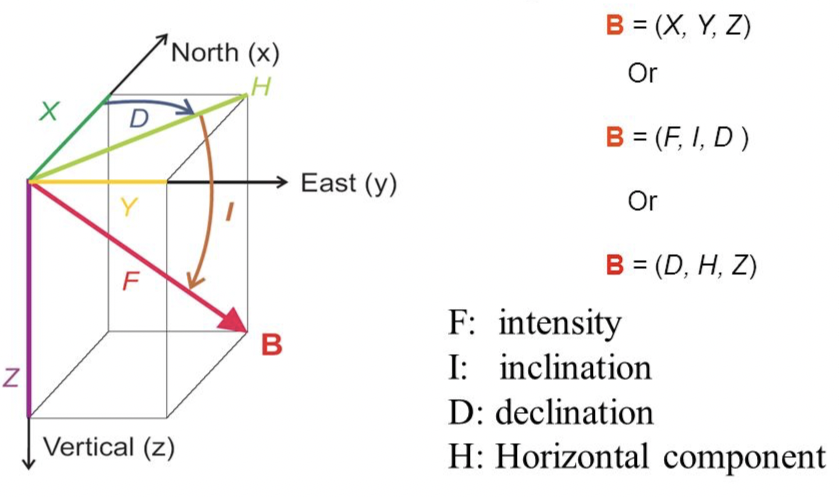
\includegraphics[width=.45\linewidth]{bilder/magnetometer_coor.png}
    \caption{Coordinate system used when measuring the geomagnetic field.}\label{fig:magnetometer_coor}
\end{figure}

\subsection{Slow variations}
The magnetic field we measure with the magnetometers can be split up into different contributors. Among the slow variations in the magnetic field we have (1) secular variations which are continuous drift in the intensity and direction of the field and the changes are noticeable over relatively short timescales (tens of years). It can be seen as a gradual monotonic decline in field intensity, about \(20\% \) over the last \(500\) years. We have also got (2) geomagnetic excursions. This is radical swings in field direction accompanied by a decrease in field strength, with a timescale of tens to thousands of years. The magnetic pole position changes by up to \SI{45}{\degree} but it is not usually recorded around the entire world. In most cases, the field regenerates with the original polarity. A (3) geomagnetic reversal is when the magnetic north and south poles are interchanged. We have had \(183\) reversals over the last \(83\) million years, with the most recent one occurring \(\num{780000}\) years ago. The occurrence is statistically random.

\subsection{Fast variations}
Fast variations are often more interesting when looking at magnetometer data. They happen on the time scales of a few minutes to several days and originate externally, e.g.\ due to currents in the ionosphere and magnetosphere. Fast variations may be a solar storms or substorms, geomagnetic pulsations or it may be solar quiet (\(S_q\)) variations. These are neutral winds that exist in the ionosphere (driven by solar heating, lunar \& solar tides). The winds will then create movement in electric charges in the E-region ionosphere, thus making current systems, and the magnetometer stations around the world can be used to track these currents. The \(X\)-component points to geographic north and at low latitudes this component have a single maximum near midday, being almost constant at night. In mid-latitude we see a decrease in the midday maximum, and at \(\sim\SI{35}{\degree}\) we see a double wave. The higher latitude have a single minimum around noon. The \(Y\)-component pointing to the east have, in the northern hemisphere, a morning maximum and afternoon minimum, with the opposite being the case for the southern hemisphere. The \(Z\)-component, which points down, have at noon a minimum in the northern hemisphere and a maximum in the southern hemisphere, with the greatest amplitudes in the mid-latitudes. At night this component is negligible.

\begin{definition}[Equivalent current]\label{def:equivalent_current}
    Infinite current that would produce the observed overhead magnetic perturbations.
\end{definition}
We want to reconstruct the ``equivalent current'' (\cref{def:equivalent_current}) in the E-region in the ionosphere which would produce the observed \(S_q\) variation in \(\gf{B}\). An infinite plane current has \(B=\mu_0J_s/2\), which will be independent from the distance to the sheet. This is not such a bad approximation: \(\sim 70\% \) of horizontal magnetic perturbation comes from the current within a \(\SI{600}{\kilo\metre}\times\SI{600}{\kilo\metre}\) area centered on zenith. What we end up with from this is a current system described in \cref{fig:solar_quiet}
\begin{enumerate}[\(\bullet \)]
    \item Two currents cells, around foci at \(\pm\SI{30}{\degree}\) MLAT
    \item Anticlockwise vortex in northern hemisphere, clockwise in southern hemisphere
    \item Flow from dawn to dusk at equator
    \item Both cells enhance each other at the equator \(\rightarrow \) eastward current (equatorial electrojet)
\end{enumerate}
In \cref{fig:solar_quiet}, (a) \& (b) are measured (\(S_q^0+S_q^p\)), where \(S_q^0\) is an extrapolation of the midlatitude \(S_q\) system and \(S_q^p\) is the solar quiet polar current. This shows a clear 2-cell pattern. (c) \& (d) are inferred (\(S_q^p\)). This is also a 2-cell pattern, with a uniform current flow across the polar cap, parallel to the midnight noon meridian. \(S_q^p\) is believed to be driven by external sources (magnetosphere, IMF).
\begin{figure}[t]
    \centering
    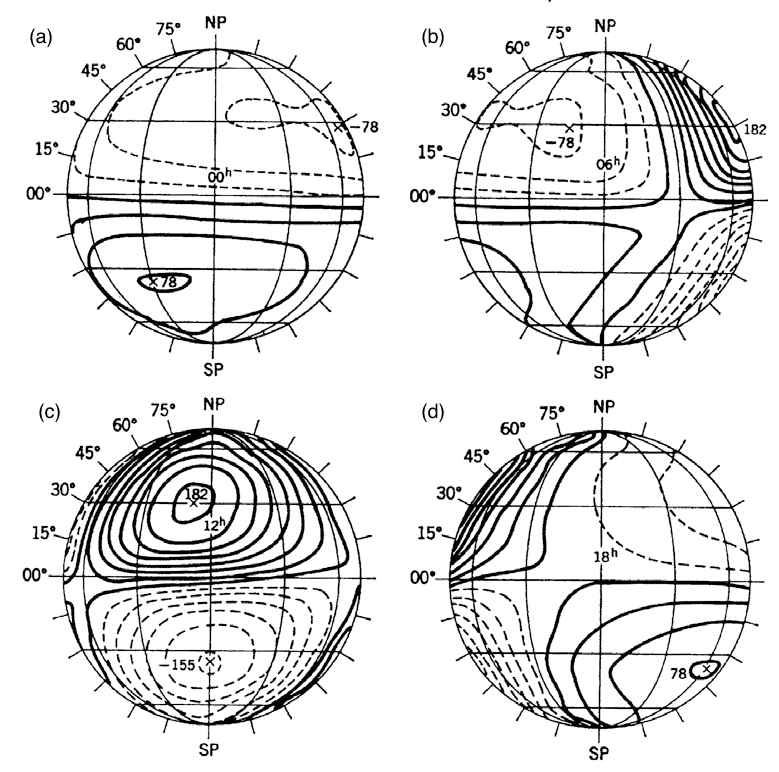
\includegraphics[width=.65\linewidth]{bilder/L3_solar_quiet.png}
    \caption{\(S_q\) current systems.}\label{fig:solar_quiet}
\end{figure}
We get geomagnetic pulsations when MHD waves enter the magnetic field. They make the field lines resonate since the field lines are fixed in the conducting ionosphere. Each field line has a natural resonating frequency which depends on field line length and plasma density profile along the field line.

\section{Magnetic \(L\)-value}
\begin{definition}[Magnetic \(L\)-value]\label{def:mag_L_value}
    The magnetic \(L\)-value describes the distance at which a particular magnetic field line crosses the equatorial plane.
\end{definition}
\noindent The magnetic \(L\)-value (sometimes called ``\(L\)-shell'') can be a convenient way to describe locations in geospace. It is derived from considering an observation point \(P\) on the Earth. We can trace a magnetic field line out to the equatorial plane. From \cref{fig:magnetic_L_value} we have that \(\gf{B}\) is always parallel to field line and the equation
\begin{equation*}
    \tan\alpha=B_\lambda/B_r=-\cos\lambda_m/2\sin\lambda_m=r\tn{d}\lambda_m/\tn{d}r
\end{equation*}
From this we get
\begin{equation*}
    \Rightarrow \frac{\tn{d}r}{r}=-2\frac{\sin\lambda_m}{\cos\lambda_m}\tn{d}\lambda_m
\end{equation*}
A solution to this equation is
\begin{equation*}
    \ln r=2\ln(\cos\lambda_m)+C
\end{equation*}
where \(C\) is an arbitrary constant of integration. When \(\lambda_m=0\) (equatorial plane) we have \(r=r_0\).
\begin{align*}
    \therefore C&=\ln r_0\\
    \therefore r&=r_0\cos^2\lambda_m
\end{align*}
For a plane on Earth’s surface (\(r=R_E\)) the field line through this point reaches the equatorial plane at distance
\begin{equation*}
    r_0=\frac{R_E}{\cos^2\lambda_m}
\end{equation*}
We define the ratio \(r_0/R_E=L\), i.e.\
\begin{equation*}
    L=\cos^{-2}\lambda_m\quad\Rightarrow\quad\lambda_m=\arccos\left(\sqrt{\frac{1}{L}}\right)
\end{equation*}
At Tromsø, \(\lambda_m=67\degree\Rightarrow \boxed{L=6.55}\) (\(r_0\approx 41730\si{\kilo\metre}\)).

\begin{figure}[t]
    \centering
    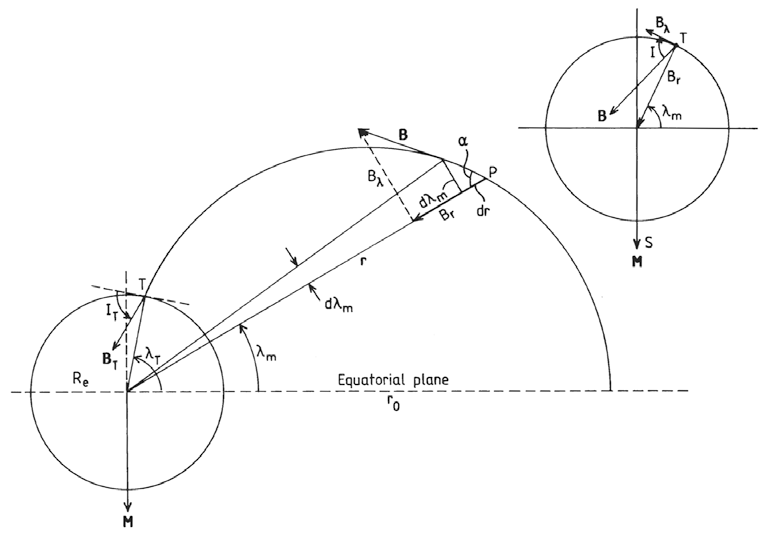
\includegraphics[width=.6\linewidth]{bilder/L3_magnetic_L_value.png}
    \caption{Magnetic \(L\)-value.}\label{fig:magnetic_L_value}
\end{figure}

\section{\(E\)-field mapping along conducting field lines}
We now look at how we can map the \(E\)-field, and our main assumption is that we have conducting field lines. We consider an electric field created in the ionosphere (\cref{fig:E_field_mapping}). We map this electric field into the equatorial plane. We will map the azimuthal and meridional components separately. We first consider two magnetic field lines separated in azimuth (\cref{fig:E_field_mapping1})
\begin{align*}
    \ell_{i\phi}&=\tn{ separation in ionosphere}\\
    L_{m\phi}&=\tn{ separation in equatorial plane}
\end{align*}
The separation is constant along geomagnetic latitudes.
\begin{equation*}
    \ell_{i\varphi}=R_E\cos\lambda_m\tn{d}\phi
\end{equation*}
\begin{equation*}
    L_{m\phi}=r_0\tn{d}\phi=\frac{R_E}{\cos^2\lambda_m}\tn{d}\phi
\end{equation*}
We assume that the line connecting the ionosphere to the equatorial plane is an equipotential
\begin{equation*}
    \Phi_\phi=E_{i\phi}\ell_{i\phi}=E_{m\phi}L_{m\phi}
\end{equation*}
where \(E_{i\phi}\) is the azimuthal component of \(\gf{E}\) in the ionosphere (equivalent for \(E_{m\phi}\)).
\begin{equation*}
    \frac{E_{i\phi}}{E_{m\phi}}=\frac{L_{m\phi}}{\ell_{i\phi}}=\frac{1}{\cos^3\lambda_m}=L^{3/2}
\end{equation*}
\textbf{E.g.}\ Tromsø: \(L\sim 6.5\Rightarrow \) enhancement of \(16.6\). Equatorial field of \(\SI{1}{\milli\volt\metre^{-1}}\) is enhanced to \(\SI{16.6}{\milli\volt\metre^{-1}}\) in the ionosphere.

We then look at two field lines separated in the meridian (\cref{fig:E_field_mapping2}). Consider two field lines separated by an angle \(\lambda_m\) in the meridional plane
\begin{align*}
    \ell_{i\lambda}&=\tn{ separation in ionosphere}\\
    L_{m\lambda}&=\tn{ separation in equatorial plane}
\end{align*}
From earlier, we have \(r_0=R_E/\cos^2\lambda_m\)
\begin{equation*}
    \ell_{i\varphi}=R_E\tn{d}\lambda_m\sin I
\end{equation*}
\begin{equation*}
    L_{m\phi}=\tn{d}r_0=2R_E\frac{\sin\lambda_m}{\cos^3\lambda_m}\tn{d}\lambda_m
\end{equation*}
The mapping ratio then become
\begin{align*}
    \frac{E_{i\lambda}}{E_{m\lambda}}&=\frac{L_{m\lambda}}{\ell_{i\lambda}}=\frac{2\sin\lambda_m}{\cos^3\lambda_m\sin I}\\
    &=\frac{2\sin\lambda_m}{\cos^3\lambda_m}\frac{1}{2\tan\lambda_m\cos I}\\
    &=\frac{1}{\cos^2\lambda_m}\frac{1}{\cos I}=\frac{1}{\cos^2\lambda_m}\sqrt{4\tan^2\lambda_m+1}\\
    &=L\sqrt{4\tan^2\lambda_m+1}=2L\sqrt{L-\frac{3}{4}}
\end{align*}
\textbf{E.g.}\ Tromsø: \(L=6.5\Rightarrow \) mapping ratio \(=31.2\). Equatorial field of \(\SI{1}{\milli\volt\metre^{-1}}\) is enhanced to \(\SI{31.2}{\milli\volt\metre^{-1}}\) in the ionosphere.

\begin{figure}[t]
    \centering

    \begin{subfigure}[t]{.49\linewidth}
        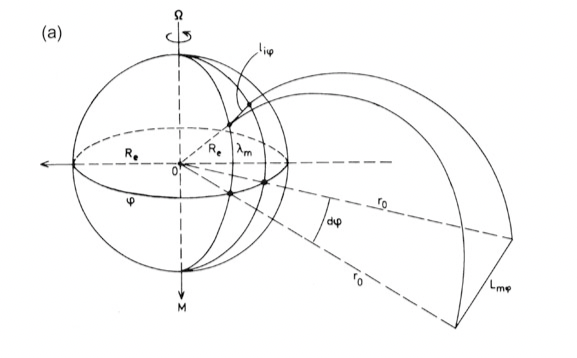
\includegraphics[width=.95\linewidth]{bilder/L3_E_field_mapping.png}
        \caption{}\label{fig:E_field_mapping1}
    \end{subfigure}
    \begin{subfigure}[t]{.49\linewidth}
        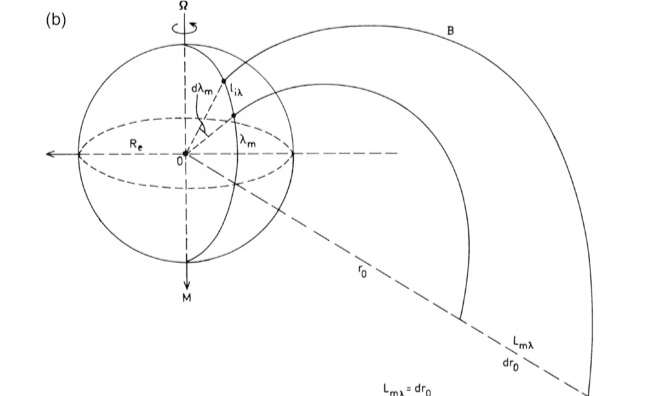
\includegraphics[width=.95\linewidth]{bilder/L3_E_field_mapping2.png}
        \caption{}\label{fig:E_field_mapping2}
    \end{subfigure}

    \caption{\(E\)-field mapping along conducting field lines.}\label{fig:E_field_mapping}
\end{figure}


\chapter{Auroral processes}
\begin{remark}
    Section made from lectures done by Lindis Bjoland. Other sources are \citet{1995Itsp} --- parts of chapter 14 --- \& \citet{BrekkeAsgeir2013Potu} --- chapter 6.8 and chapter 7 part 11 to 12.
\end{remark}
\textbf{Plan for the week}
\begin{enumerate}[\(\bullet \)]
    \item \emph{Monday} --- Introduction about auroral emissions
    \item \emph{Tuesday} --- Particle precipitation
    \item \emph{Wednesday} --- Auroral distribution in space/time
    \item \emph{Friday} --- Exercises/info.\ about field work
\end{enumerate}
High energy particles may use 20 mins to reach the Earth, while the solar wind takes 2--4 days.\\

\begin{minipage}{.49\linewidth}
\textbf{Dayside}
    \begin{enumerate}[\(\triangleright \)]
    \item source is the solar wind
    \item soft precipitation (\(<\SI{1}{\kilo\electronvolt}\))
    \item mainly red emission
    \item high peak emission height
\end{enumerate}\end{minipage}
\begin{minipage}{.49\linewidth}
\textbf{Nightside}
\begin{enumerate}[\(\triangleright \)]
    \item source is the magnetotail
    \item hard precipitation (\(1-\SI{15}{\kilo\electronvolt}\))
    \item mainly green emission
    \item low peak emission height
\end{enumerate}\end{minipage}

\section{Auroral emissions}
\textbf{E.g.:} Forbidden transition of \(\SI{5577}{\angstrom}\) \\
\([OI]~2p^4\prescript{1}{}{D}-2p^4\prescript{1}{}{S}\) where \([~]\) denote a forbidden transition.
\begin{equation*}
    \underset{\substack{\uparrow \\ \tn{shell}}}{2}\underset{\substack{\uparrow \\ \tn{orbital}}}{p}^4
\end{equation*}
where \(4\) here denotes the number of electrons.
\begin{enumerate}[\(\bullet \)]
    \item \(n=2\): principal quantum number
    \item \(\ell \): azimuthal quantum number (\(\ell=0, 1, 2, \ldots , (n-1)\))
    \item \(\prescript{1}{}{D}/\prescript{1}{}{S}\): two terms in the ground configurations with multiplicity \(2S+1\)
    \item I\@: unionized
    \item II\@: singly ionized
\end{enumerate}
Dissipation in the ionosphere: \begin{enumerate}
    \item excitation \(\Rightarrow \) auroral emissions
    \item ionization \(\Rightarrow \) enhancement of conductivity
    \item collisions/heating
\end{enumerate}

\subsection{Cross section}
The cross section is used to described the likelihood of a favorable collision. In the high energy tail there will be particles that need to loose energy before they are able to excite, and each ion behave differently. The cross section will decrease towards higher energies from the maximum as can be seen in \cref{fig:L4_cross_section}.
\begin{figure}[t]
    \centering
    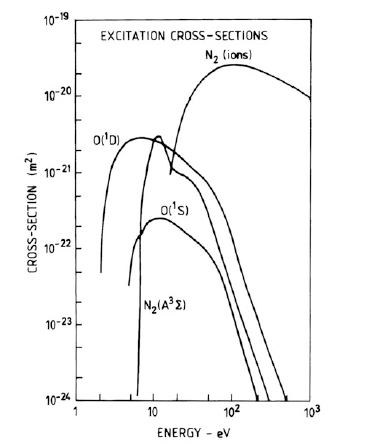
\includegraphics[width=.6\linewidth]{bilder/L4_cross_section.png}
    \caption{}\label{fig:L4_cross_section}
\end{figure}

\subsection{Atomic oxygen energy levels}
The difference in excitation energy implies that the intensity ratio between green (\(\SI{5577}{\angstrom}\)) and red (\(\SI{6300}{\angstrom}\)) emission decreases with decreasing energy of precipitating particles. We end up with, when looking at the intensities of the light, the fraction
\begin{equation*}
    \frac{I(\SI{5577}{\angstrom})}{I(\SI{6300}{\angstrom})}=\frac{\tn{green}}{\tn{red}}
\end{equation*}
which takes in the intensities of the two wavelengths. As mentioned, this will decrease with decreasing energy of the electrons. This means that lower energy will give a greater chance of red light.
Impact excitation
\begin{equation*}
    \tn{O}(\prescript{3}{}{P})+e\rightarrow \tn{O}(\prescript{1}{}{S})+e
\end{equation*}
followed by an emission of either \(\SI{5577}{\angstrom}\) or \(\SI{2972}{\angstrom}\). Red doublet is described by
\begin{equation*}
    \tn{O}(\prescript{3}{}{P})+e\rightarrow \tn{O}(\prescript{1}{}{D})+e
\end{equation*}
followed by emission of the red line
\begin{equation*}
    \tn{O}(\prescript{1}{}{D})\rightarrow
\end{equation*}
\begin{equation*}
    \boxed{\SI{1}{\electronvolt}=\num{1.602e-19}\si{\joule},\quad E=h\nu=\frac{hc}{\lambda} [\si{\joule}]}
\end{equation*}

\subsection{Oxygen emission}
The {\color{red}red} color at \(\lambda\approx\SI{6300}{\angstrom}\) has its peak at \(\sim\SI{230}{\kilo\metre}\). It comes from an atomic oxygen \(\prescript{3}{}{P}\rightarrow\prescript{1}{}{D}\) transmission. Due to the long lifetime of the excited state \(\tn{O}(\prescript{1}{}{D})\) (\SI{110}{\second}), the excitation peaks at \(\sim\SI{100}{\kilo\metre}\). Quenching due to the long lifetime make the peak emission height be at above \SI{200}{\kilo\metre}. Most likely due to atom-interchanging reactions. \begin{equation*}
    \tn{N}(\prescript{2}{}{D})+\tn{O}_2\rightarrow \tn{NO}+\tn{O}(\prescript{1}{}{D})
\end{equation*}
The {\color{green}green} color at \(\lambda\approx\SI{5577}{\angstrom}\) has it peak at \(\sim\SI{110}{\kilo\metre}\). It comes from an atomic oxygen \(\prescript{1}{}{D}\rightarrow\prescript{1}{}{S}\) transmission, and the excited state has a much lower lifetime than the red has. Excited state \(\tn{O}(\prescript{1}{}{S})\) has a lifetime of \(\SI{0.7}{\second}\). The most likely cause of this excitation is an ionized oxygen molecule combined with an electron.
\begin{equation*}
    \tn{O}_2^+ + e\rightarrow \tn{O}+\tn{O}(\prescript{1}{}{S})
\end{equation*}


\subsection{Nitrogen emission}
One of the best understood emissions is related to excitation of the \(\tn{N}_2^+\) ion, more specifically to the \(B^2\Sigma_\mu^+\) state which has a maximum cross-section of excitation close to 100 eV. It can be seen as emissions at \(\lambda\approx\SI{3914}{\angstrom}\) and \(\lambda\approx\SI{4278}{\angstrom}\). Because they are spontaneous emissions, radiation occurs at the incidence of primary and secondary particles within \(10^7\) s. The {\color{blue}blue} color at \(\lambda\approx\SI{4278}{\angstrom}\) has its peak height of \SI{90}{\kilo\metre}. The excited state has a lifetime of \SI{70}{\nano\second}.
\begin{equation*}
    \tn{N}_2+(e\tn{ or }\tn{H}^+)\rightarrow{(\tn{N}_2^+)}^*+(e'\tn{ or }\tn{H}^{+'})+e
\end{equation*}
\begin{equation*}
    {(\tn{N}_2^+)}^*\rightarrow \tn{N}_2^++(\SI{3914}{\angstrom}\tn{ and }\SI{4278}{\angstrom})
\end{equation*}
\begin{equation*}
    e'=e-\SI{36}{\electronvolt}/\tn{H}^{+}=\tn{H}^{+'} -\SI{36}{\electronvolt}
\end{equation*}
\begin{align*}
    \lambda_{3914} \tn{ create }25\tn{ ion pair per photon}\\
    \lambda_{4278} \tn{ create }75\tn{ ion pair per photon}
\end{align*}
Since there is a relationship between how many photons are created and the energy of the incident electron, namely
\begin{equation}\label{eq:L4_number_of_photons_per_ion}
    \eta(\SI{3914}{\angstrom})=0.02\frac{n(\tn{N}_2)}{n}\frac{\varepsilon_0}{W}
\end{equation}
where \(\eta \) is the number of photons created, 0.02 is the ratio of photons created (according to AB 1 photon per 50 ion pairs, hence 0.02), \(n\) describe number densities of the molecule and the total number density in the atmosphere at the height of the emission, \(\varepsilon_0\) is the initial energy of the electron and \(W\) is the mean ionization energy (about 35--36 eV).

So, emission intensity is directly proportional to the energy flux of primary electrons. The process is independent of energy at \(0.5\)--\(\SI{20}{\kilo\electronvolt}\). Dawn/dusk \(\tn{N}_2^+\) may absorb the blue in the sunlight and re-emit it to make what is called resonant scattering.
\begin{figure}[ht]
    \centering
    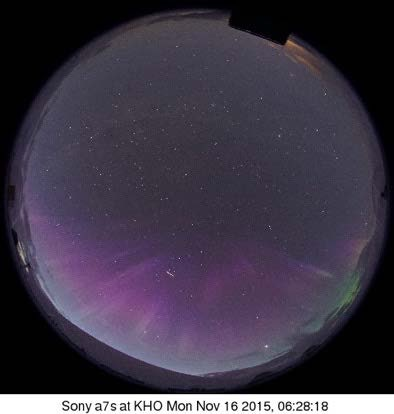
\includegraphics[width=.6\linewidth]{bilder/L4_resonant_scattering.jpg}
    \caption{Resonant scattering at KHO\@. Blue emission at the top part of the auroral curtain at dawn.}\label{fig:L4_resonant_scattering}
\end{figure}

\subsection{Proton aurora}
\begin{enumerate}[\(\bullet \)]
    \item weak {\color{blue}blue} emissions at \SI{4861}{\angstrom} (\(\tn{H}_\beta \)) and {\color{red}red} emission at \SI{6563}{\angstrom} (\(\tn{H}_\alpha \)) as excitations of a neutral hydrogen.
    \item intensity range is between \(50\)--\(\SI{300}{\ray}\)
    \item will look like diffuse aurora since they may get hold of an electron, making them neutral for a while
\end{enumerate}
\begin{align*}
    \tn{X}+\tn{H}^+&\rightarrow \tn{X}^+\tn{H}^*\\
    \tn{H}^*&\rightarrow \tn{H}+h\nu \\
    \tn{H}+\tn{X}&\rightarrow \tn{H}^++\tn{X}+e
\end{align*}

\section{Precipitation patterns}
We divide the energies of the particles into three zones: high, medium and low energy particles. High energy is defined to be \(>\SI{20}{\kilo\electronvolt}\) and we see higher number flux from 4 to 12 MLT\@. Medium energy is defined to be \(0.5\)--\(\SI{20}{\kilo\electronvolt}\) and they are often auroral zone particles with the highest flux on the nightside. Low energy is defined to be \(<\SI{1}{\kilo\electronvolt}\) and the are associated to high flux due to their more direct entry.

The particles entering in the cusps are entering in a minima in the magnetic field between the sunward and tailward field lines, and are therefore most often of lower energy than those entering on the nightside, and hence this is mainly sub-visual precipitation. The cusps are direct entry points of magnetosheath plasma into the atmospheres, and they are located at \(\sim 11\)--\(13\) MLT with a width of \(\sim\SI{1}{\degree}\). \Cref{fig:L4_maps_precipitation_pattern} show a map of precipitation patterns for the dayside of the northern hemisphere
\begin{enumerate}[\(\bullet \)]
    \item {\color{red}cusp}: proton and electron precipitation at low energies
    \item {\color{green}mantle}/{\color{blue}LLBL} (lower latitude boundary layer): soft electron precipitation from the magnetosheath
    \item {\color{cyan}CPS} (central plasma sheet)/{\color{blue!50}BPS} (boundary plasma sheet): medium energy electron precipitation from the plasma sheet
    \item \textcolor{yellow}{\contour{black}{polar rain}}: spatially homogenous electron precipitation at a few hundred \si{\electronvolt} energies
\end{enumerate}
\begin{figure}[t]
    \centering
    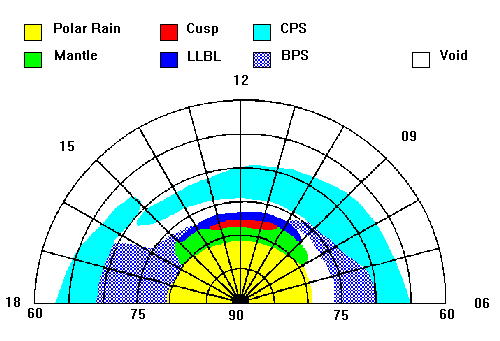
\includegraphics[width=.6\linewidth]{bilder/L4_maps_precipitation_pattern.png}
    \caption{Maps of average precipitation patterns.}\label{fig:L4_maps_precipitation_pattern}
\end{figure}
Some challenges connected to the mapping of precipitation patterns are energy convection and dispersion, field-aligned acceleration and gradient and curvature drifts.

\section{Auroral intensities --- the Rayleigh unit}
For reference, we have that the intensity of the night sky is \(\sim \SI{250}{\ray}\), while the visibility threshold of a human eye is \(\sim \SI{1}{\kilo\ray}\). Auroral intensities are up to \(\sim \SI{1000}{\kilo\ray}\), where the unit \si{\ray} is defined as
\begin{equation}\label{eq:rayleigh_definition}
    \si{\ray}=10^{10}\frac{\tn{photons}}{\si{\metre^2\second}}=4\pi\tn{I}=\int_0^\infty F(\gf{r})\tn{d}r
\end{equation}
where \(F(\gf{r})\) is the volume emission rate. The intensity \(I\) is defined as
\begin{equation*}
    I(X(\lambda))=\frac{\pi}{10^6}\int_0^\infty j(E)P(E)\tn{d}E
\end{equation*}
where \(X(\lambda)\) is a gas \(X\) at a wavelength \(\lambda \), \(E\) is energy, \(j(E)\) is the differential electron or proton energy spectrum and \(P(E)\) is the total number of photons for gas \(X\) at wavelength \(\lambda \). Due to the viewing geometry and the transparency of the aurora, an observer sees surface brightness of the aurora. Rayleigh unit describes this apparent brightness. The distribution of the auroral intensities is shown in \cref{fig:L4_dist_of_auroral_intensities}.
\begin{figure}[t]
    \centering

    \begin{subfigure}[t]{.47\linewidth}
        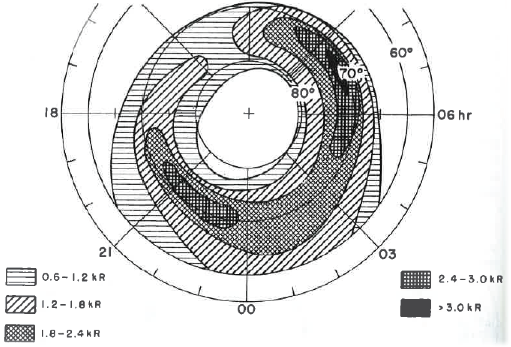
\includegraphics[width=.95\linewidth]{bilder/L4_dist_of_auroral_intensities.png}
        \caption{}\label{fig:L4_dist_of_auroral_intensities}
    \end{subfigure}
    \begin{subfigure}[t]{.47\linewidth}
        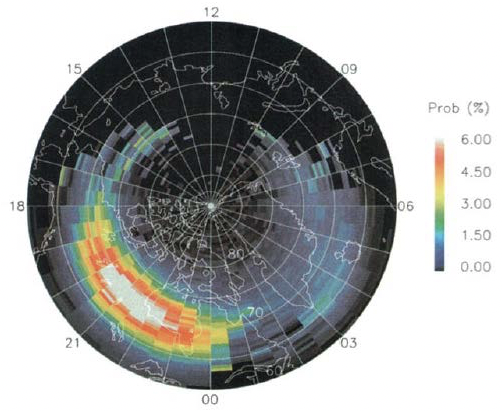
\includegraphics[width=.95\linewidth]{bilder/L4_intensities_darkness.png}
        \caption{}\label{fig:L4_intensities_darkness}
    \end{subfigure}

    \caption{\textbf{\subref{fig:L4_dist_of_auroral_intensities}}: Distribution of auroral intensities. \textbf{\subref{fig:L4_intensities_darkness}}: Intensities as it appears in darkness/light.}\label{fig:L4_intensity_distributions}
\end{figure}

\section{Auroral shapes and forms --- auroral substorms}
\subsection{Currents in the ionosphere}
In order to have currents, we need ion motion relative to the electrons. The velocity difference, and hence current, is strongest in the E-region where the electron motion is governed by \(\gf{E}\times\gf{B}\)-drift and the ion motion is governed by collisions with neutrals.
\(E_x\) --- primary electric field. Continues across the boundary \(\nabla\times\gf{E}=0\). Pedersen: \(\vert\vert E,\perp B\); Hall: \(\perp E,\perp B\). This leads to a more intense current along  the auroral arc. \Cref{fig:L4_E-reg_currents} show the currents in the ionosphere.
\begin{figure}[t]
    \centering
    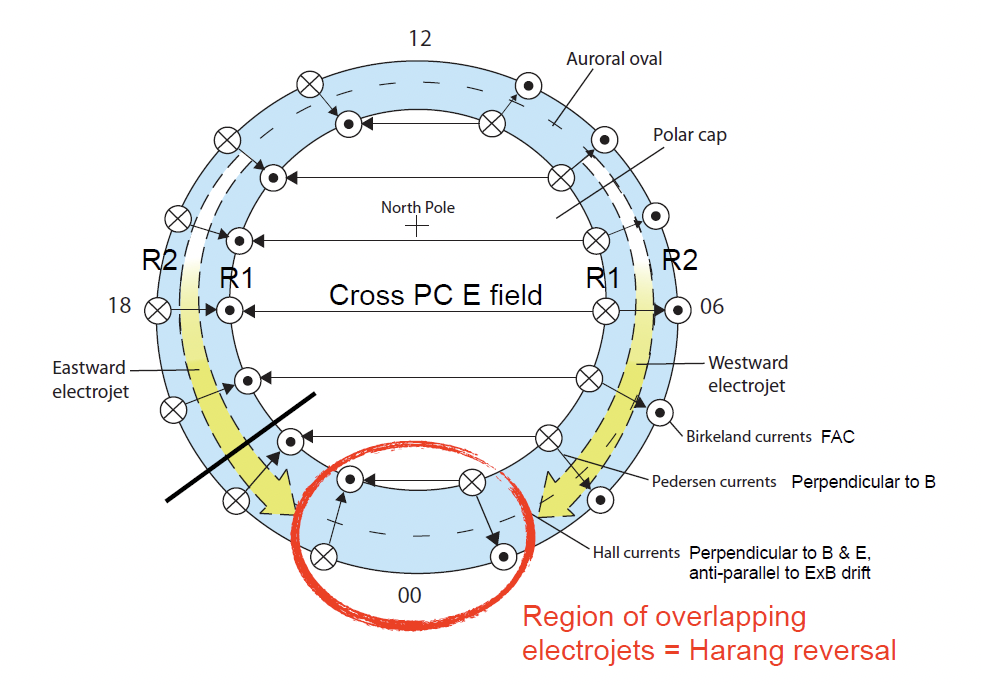
\includegraphics[width=.8\linewidth]{bilder/L4_E-reg_currents.png}
    \caption{Currents in the ionosphere.}\label{fig:L4_E-reg_currents}
\end{figure}
The different forms of aurora can be classified into (1) arcs which is east-west aligned smooth bands with widths of \(\sim 1\)--\(\SI{100}{\kilo\metre}\), (2) rays, magnetic field-aligned small features which often move along the arcs, (3) diffuse/irregular, wide-spread low luminosity distribution which often forms irregular patches of light and (4) vortical structures, spirals, curls, folds and surges, distortions of different sizes along auroral arcs.

Some key features that determine the electrodynamics of auroral structures are the background convection electric field, the relationship between the conductivities inside and outside the aurora and the field-aligned currents associated with the aurora.

The absolute value of the electric field is more intense on the equatorward side than on the poleward side of the arc. The currents of large vortex structures are fed by a converging Pedersen current from the surroundings into an upward field-aligned current. The Hall current around the precipitation region leaves the magnetic trace of upward FAC\@.

\subsection{Polar cap sun-aligned arcs}\label{subsec:sun_aligned_arcs}
This is auroras within the polar cap, pointing towards the sun. They are correlated with IMF \(B_z>0\) and occurs about 50\% of the time. They are of electromagnetic origin and are markers of velocity shear. What we have is a boundary problem, and we either have a flow reversal or a flow gradient. This ends with an electrical field that discontinues across the boundary. In steady state, we must have divergence free currents. In order to get \(\nabla\cdot\gf{j}=0\), a field aligned current is needed. Upward currents are carried by suprathermal electrons, \(E\sim 10-\SI{100}{\electronvolt}\rightarrow \) excitation \(\rightarrow \) light produced.

\subsection{The evolution of substorm aurora}
First, you enter the growth phase, in which quasi-stable arcs are drifting equatorward. The auroral onset often starts equatorward of the preexisting arc and is preceded by the auroral fading. Then comes the expansion phase, and we see auroral madness in multiple forms and scales that are bright and speedy. The last phase is the recovery phase. Here, we find patches, omega-bands and other complicated auroral structures with decaying intensity.
\begin{enumerate}
    \item morphological evolution and description of basic forms
    \item typical location of the substorm onset
    \item extent and speed of the expansion
    \item drift motion and alignments
    \item displays at different parts of the oval
    \item variations in brightness and magnetic field
    \item lifetime of the cycle \(\sim 2\) hours
\end{enumerate}
In MSP data, a substorm would look like an equatorward moving structure during the growth phase, and then followed by a brightening of the equatormost aurora. Next, a rapid poleward expansion of the aurora would fill the field of view. During recovery we see a decay in intensity.

\section{Questions --- week 5}
\begin{enumerate}
    \item [2005 EXERCISE 1]~\\\vspace{-5mm} \begin{enumerate}
        \item \textbf{The aurora can be defined as a three-step process in energy transfer. Discuss briefly the main characteristics of the different energy steps.}\\ First step is an electron that excite an ion. Next we have an ion with potential/chemical energy. At last we see the photon from the emission.
        \item \textbf{List the main phases in an auroral substorm. What characterize the auroras --- intensity, shape and colors --- in the different phases?}\\ The stages are growth (arcs start moving, mostly green), expansion (every color) and recovery (patches, intensity reduces, mostly green).
        \item \textbf{Dayside auroras are very sensitive to the orientation of the interplanetary magnetic field (IMF). Discuss location and dynamics of dayside auroras when:} \begin{enumerate}
            \item \textbf{IMF \(B_z\) is strongly northward}\\ Might reconnect other places, often dependant on \(B_y\)-component. Auroral oval contracts northward. This is when we might see sun-aligned arcs (\cref{subsec:sun_aligned_arcs}).
            \item \textbf{IMF \(B_z\) is pointing southward}\\ Easy reconnection in the equatorial plane. Get auroras on the dayside and nightside with the usual growth, expansion and recovery phases.
        \end{enumerate}
        \item \textbf{An important emission in the night time aurora comes from the following transition:}
        \begin{equation*}
            \tn{OI}~(\prescript{1}{}{S}\rightarrow\prescript{1}{}{D})
        \end{equation*}
        \textbf{Discuss the main characteristics of the emission. Why is quenching by collision important?}\\ This will give green aurora at a wavelength of \(\lambda=\SI{5577}{\angstrom}\). Quenching is important because if quenching is introduced, the ion/molecule will loose its energy before the emission takes place. For this transition, the lifetime is only \SI{0.7}{\second} so you will often see this green light, instead of having its energy being quenched away.
    \end{enumerate}
    \item [2004 EXERCISE 3]~\\\vspace{-5mm} \begin{enumerate}
        \item \textbf{Auroral intensities are usually given in units of Rayleigh [R]. Define the Rayleigh unit in terms of the number of photons hitting the detector. What is a typical value in Rayleighs for the threshold value at 5577 Å for the dark adapted eye?}\\ The definition of the unit can be found in \cref{eq:rayleigh_definition}. Threshold for green is \SI{1}{\kilo\ray}.
        \item \textbf{\Cref{fig:L4_questions} shows daytime auroral intensity measurements obtained using a meridian scanning photometer (MSP). Explain the setup for this instrument, with special care being given to the filters and photo multiplier tube (PMT).}\\ The MSP works by rotating a mirror around an axis perpendicular to the meridian plane with respect to the magnetic north/south, i.e.\ it scans in the meridian plane. Depending on th setting, the MSP will scan for either 8 or 16 s, both peak and base. For an 8 s scan it will spend 4 s rotating once and scan peak values and then the next 4 s to scan base values. A 16 s scan does an average of two scans, i.e.\ two 8 s scans averaged. All four channels in use are measured at the same time. In the MSP are photo multiplier tubes (PMTs). They work as a way of enhancing the sensitivity of the instrument. Its objective is to count photons, and it does so by having an electron potential across its length. The top, where a photon would hit, serves as a cathode, and an electron is knocked loose. Several dynodes along the length of the PMT makes sure the number of electrons that is knocked loose is increasing until they reaches the bottom, where the anode sits. The electrical impulse from the anode is then a measure of how many photons was hitting the cathode.
        \item \textbf{Make a sketch of one of the channels in \cref{fig:L4_questions} showing the cusp region, the open/closed field line boundary and the polar cap region. Also mark clearly which regions are on open and closed field lines.}\\ We use the red channel with wavelength \(\lambda=\SI{6300}{\angstrom}\). From the figure we see the OCB as the lower (equatorward) edge where blue goes to green/red since this is on the dayside. The polar cap would be the upper blue region. The cusp region is then the lower part of the non-blue areas.
        \item \textbf{Other magnetospheric boundary regions include the CPS (central plasma sheet), the LLBL (low-latitude boundary layer) and the Mantle. Describe these three boundary regions with respect to open/closed field lines, energy and flux, as well as the approximate source regions in the magnetosphere (you are free to make a drawing if needed).} \\ Can be found in \cref{fig:L4_maps_precipitation_pattern}. CPS\@: we are on closed field lines, medium to high energy particles, medium to low flux, source is the tail. LLBL\@: boundary between cusp and equatorward. Mantle: on open field lines, low energy particles, medium flux, source is magnetosheath.
        \item \textbf{The 4278 Å \([\tn{N}_2^+1NG]\) (blue) emission line can be used as an indicator for the detection of ionization. Why? What is the average energy loss per collision?}\\ The emission is directly proportional to the energy flux of primary electrons. For one photon, 75 ion pairs are created, and the number of ion pairs created are dependant on the incident energy of the precipitating electron. Therefore, we have a way of going from a measure of how many photons are created to the flux of primary electrons. The average loss per collision is about 36 eV.
        \item \textbf{If \(75\) ion-pairs are produced per photon emitted, estimate the flux needed to produce \(\SI{8}{\kilo\ray}\) of \SI{4278}{\angstrom} emission, given that the mean precipitating energy is \SI{7}{\kilo\electronvolt}.}\\ %Here, I assume that the ratio of the density of nitrogen molecules to the density of the atmosphere is
        % \begin{equation*}
        %     \frac{n(\tn{N}_2)}{n}\approx 0.80
        % \end{equation*}
        Here, I assume that the mean ionization energy is 36 eV. We may find an approximation for the number of photons created by the formula given in \cref{eq:L4_number_of_photons_per_ion}, with the simplification that we only have nitrogen molecules. %This give \(\eta(\SI{4278}{\angstrom})=2.074\). The flux \(\xi \) will then be
        We then get that the flux of photons is \(\num{8e13}\tn{photons}/\si{\metre^{2}\second}\). Multiply this by 75 and you have the flux of ions. For an electron with mean energy \(\varepsilon_0\) we get one ion and loose 36 eV, therefore, the flux \(\xi \) of electrons will be given as
        \begin{equation*}
            \xi=75\cdot 8\cdot 10^{13}\cdot\frac{36}{7000}=\num{30.85e12}\si{\metre^{-2}\second^{-1}}
        \end{equation*}
        % \begin{equation*}
        %     \xi=\num{8000}\cdot 10^{10}\cdot 2.074=\num{165.92e12}\si{\metre^{-2}\second^{-1}}
        % \end{equation*}
    \end{enumerate}
    \item [2007 EXERCISE 1] \textbf{Fast electrons \((e)\) can both ionize and excite gases in the upper atmosphere. These processes can be written symbolically in the following way:}
    \begin{equation*}
        \tn{X}+e\rightarrow {(\tn{X}^+)}^*+e_n+e'
    \end{equation*}
    \textbf{where \(\tn{X}\) is an atmospheric constituent, the asterisk \(*\) indicate that the particle is in an excited state, and \(e_n\) is a thermal electron. In such collisions fast electrons loose in average \SI{35}{\electronvolt}.}
    \begin{enumerate}
        \item \textbf{Where does this energy go? Discuss the energy budget.}\\ One electron is left out (\(e'\)), and then we have the ionization and excitation.
        \item \textbf{If we instead of \(\tn{X}\) use \(\tn{N}_2\), we get:}
        \begin{equation*}
            {\left(\tn{N}_2^+\right)}^*\rightarrow \tn{N}_2^++\left[\SI{3914}{\nano\metre}\tn{ or }\SI{4278}{\nano\metre}\right]\tn{ aurora}
        \end{equation*}
        \textbf{These emissions are called the first negative band system. Why are these bands important in auroral studies?}\\ We can get an estimation of the number of ions in the ionosphere, due to the 25/75 pairs of ions created per photon emitted. We loose \SI{35}{\electronvolt} per ion.
        \item \textbf{Estimate the flux needed to produce \SI{5}{\kilo\ray} of \SI{3914}{\nano\metre} emission, given that the mean precipitation energy is \SI{10}{\kilo\electronvolt}.}\\
        \begin{align*}
            \num{5e13}\tn{ photons/}\si{\metre^2\second}\Rightarrow\num{125e13}\tn{ ions}\\
            35\cdot\num{125e13}\tn{ ions}\rightarrow \num{4375e9}\tn{ electrons/}\si{\metre^2\second}
        \end{align*}
    \end{enumerate}
    \item \textbf{Discuss the excitation mechanism for proton auroras, i.e.\ the hydrogen lines in the auroral spectrum. Why are observations of these emissions so important in space physics?}\\ A proton can pick up an electron to form a fast neutral hydrogen atom, making it free to move across magnetic field lines until a new collision occurs and the atom is stripped of its electron.
    \begin{align*}
        \tn{X}+\tn{H}^+&\rightarrow \tn{X}^++\tn{H}^*\\
        \tn{H}^*&\rightarrow \tn{H}+h\nu \\
        \tn{H}+\tn{X}&\rightarrow \tn{H}^++\tn{X}+e_n
    \end{align*}
    In the neutral state a hydrogen atom can be excited to emit either \(\tn{H}_\alpha \) (6563 Å) or \(\tn{H}_\beta \) (4861 Å). Due to the velocity of an \(\tn{H}^*\) atom along the field line, the wavelengths are Doppler shifted which can be measured, and hence also the velocities of the particles.
    \item \textbf{List the main characteristics of the dayside auroral-oval auroras.}\\ On the dayside there is easier access for the precipitation particles, so intensities can often be lower due to the particles having, on average, lower energy. On the other hand, the flux is higher. This means that for instance the red light, coming from excited states with long lifetimes which for that reason are prone to quenching, have a higher chance of being visible. This makes the dayside aurora appear more red and span a greater range in altitude.
\end{enumerate}
\begin{figure}[ht]
    \centering
    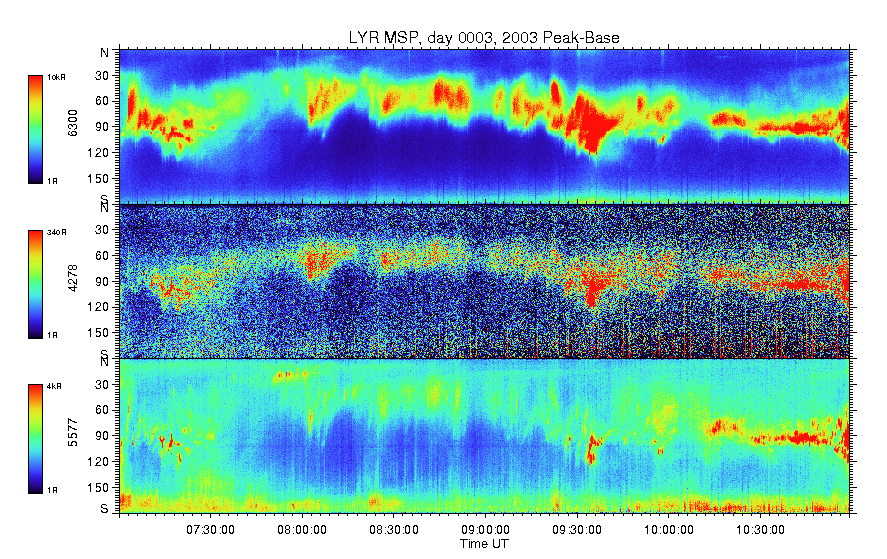
\includegraphics[width=.9\linewidth]{bilder/L4_questions.png}
    \caption{}\label{fig:L4_questions}
\end{figure}


\chapter{Field work}
\section{Monday}
\subsection{MSP --- Meridian Scanning Photometer}
\begin{enumerate}[\(\bullet \)]
    \item 30° off Meridional line since we want mag.\ mer.\ line.
    \item 4 photometers
    \item photon multiplier tube\begin{enumerate}[\(\triangleright \)]
        \item acc.\ electrons
        \item sees individual photons
        \item is cooled down to \SI{-20}{\celsius} to reduce thermal noise
    \end{enumerate}
\end{enumerate}

\subsection{Auroral forecast}
\begin{enumerate}[\(\bullet \)]
    \item Look at DSCOVR data
    \item \(B_z\) most influential
    \item \(B_y\) to affect polar cap convection pattern\begin{enumerate}[\(\triangleright \)]
        \item L1 at \(\num{1.5e9}\si{\metre}\). Solar wind: \SI{400}{\kilo\metre\second^{-1}}
        \item \(\rightarrow 1\) Hour
    \end{enumerate}
    \item Now look at SuperDARN to find convection time
    \item Typical convection speed: \(v_c\sim 300-\SI{500}{\metre\second^{-1}}\)
    \item Distance: (ionosphere height is trivial at \num{200000}~\si{\kilo\metre})\begin{equation*}
        30\degree \rightarrow\frac{\pi}{2}\frac{1}{3}\Rightarrow d=\frac{\pi}{6}R_E,\quad R_E=\SI{6600}{\kilo\metre}
    \end{equation*}
    \item Time:\begin{equation*}
        t=\frac{\pi}{6}\frac{R_E}{v_c}\approx \SI{8639}{\second}\approx 2.4\tn{ h},\quad v_c=\SI{400}{\metre\second^{-1}}
    \end{equation*}
\end{enumerate}
\begin{figure}[ht]
    \centering
    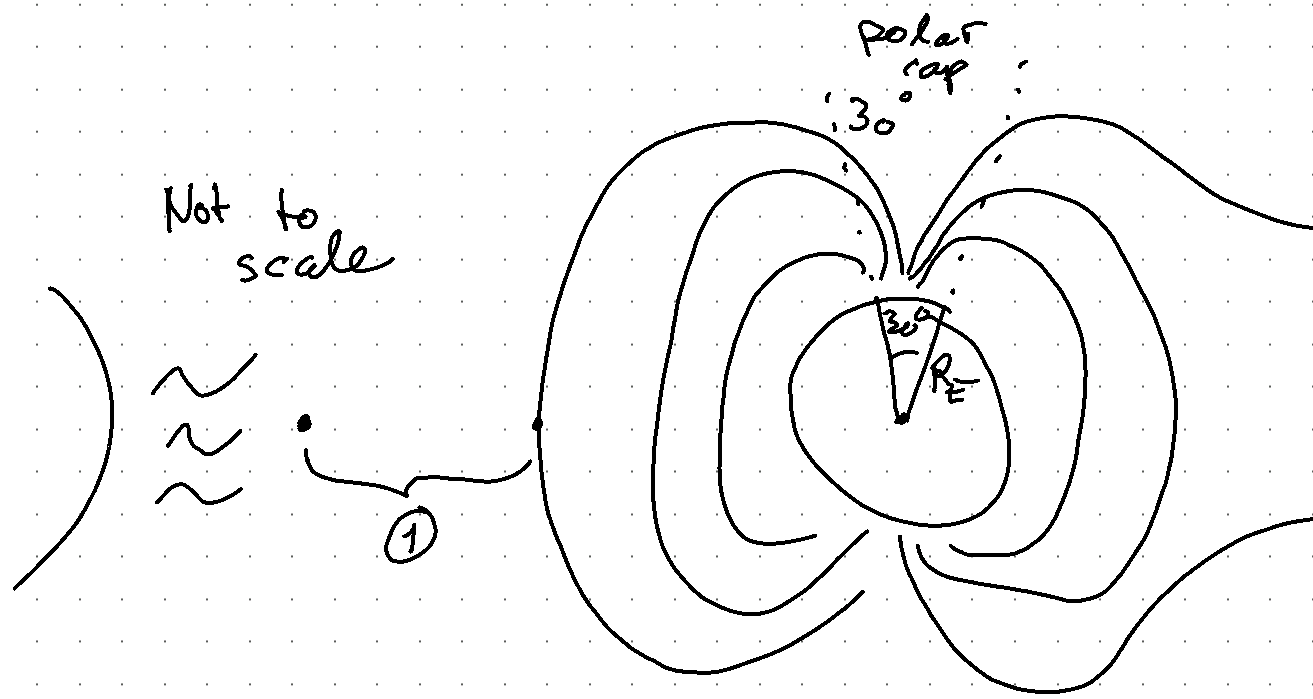
\includegraphics[width=.7\linewidth]{bilder/L5_field_work_monday.png}
    \caption{}\label{fig:L5_field_work_monday}
\end{figure}

\section{Tuesday}
Trigonometry the whole day more or less.

\section{Wednesday}
\subsection{The 1m GREEN}
\begin{enumerate}[\(\bullet \)]
    \item has a \SI{1}{\milli\metre} slit, and the narrower it is the higher the resolution, but you will also get less light in
    \item the angle the light enters the grating at is \SI{6.735}{\degree} from the normal
    \item blaze angle for the grating is \SI{30}{\degree}
    \item scans from \(420-\SI{430}{\nano\metre}\) which is where the Nitrogen line are located, and from \(480-\SI{490}{\nano\metre}\) where the Hydrogen \(H_\beta \) is part of the Balmer series
    \item for the most efficiency, we look for angles close to the blaze angle for how tilted he grating is\begin{enumerate}[\(\triangleright \)]
        \item 2.\ order for the \(H_\beta \) (\SI{36}{\degree}) where it has a \(\SI{3}{\angstrom/\milli\metre}\) resolution\begin{equation*}
            \fracd[x]{\lambda}=3.0\frac{\si{\angstrom}}{\si{\milli\metre}}
        \end{equation*}
    \end{enumerate}
\end{enumerate}

\section{Thursday}
\subsection{Absolute calibration}
\begin{enumerate}[\(\bullet \)]
    \item done once a year
    \item goal is to convert data into a usable unit
    \item set up shown in \cref{fig:L5_field_work_thursday}
\end{enumerate}
\begin{figure}[t]
    \centering
    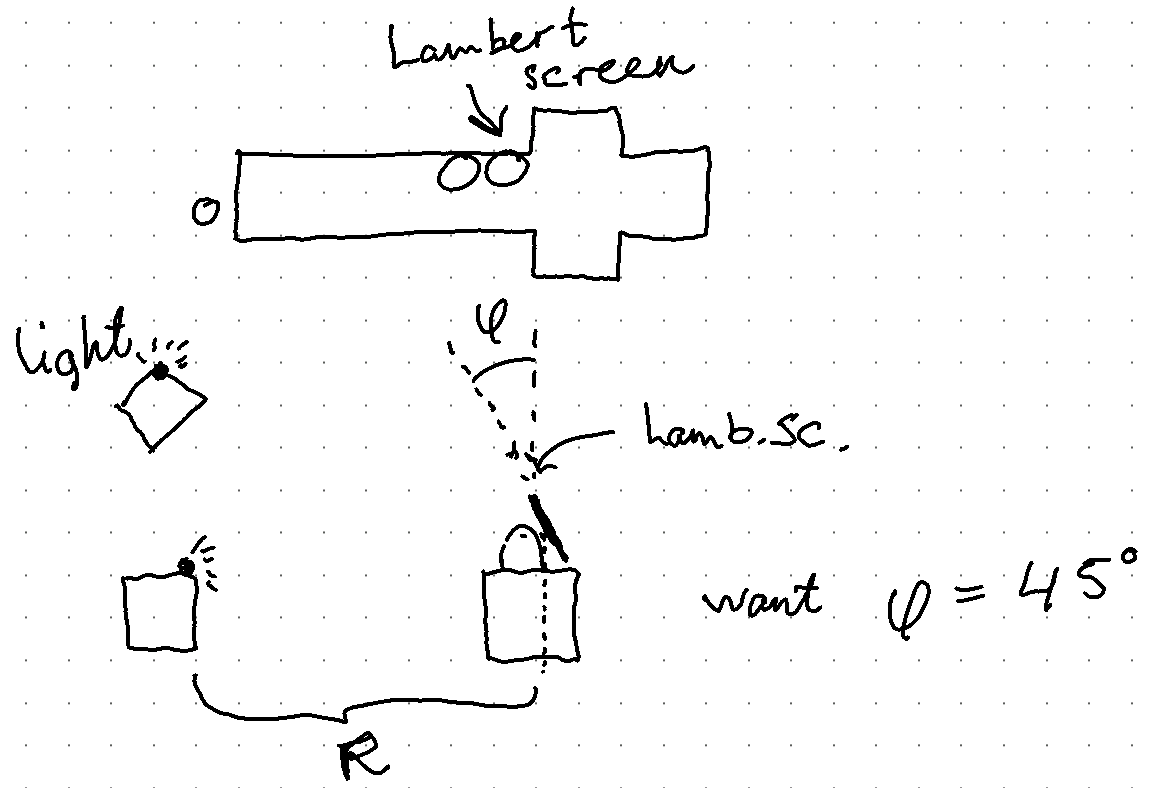
\includegraphics[width=.8\linewidth]{bilder/L5_field_work_thursday.png}
    \caption{Set up of the Tungsten lamp relative to the domes at KHO.}\label{fig:L5_field_work_thursday}
\end{figure}
So how do we do the conversion? If \(B_{ph}\) is the is the true luminance in SI units, then
\begin{equation*}
    B_{ph}=I_R\frac{1}{4\pi}10^4~\left[\frac{\tn{photon}}{\si{\metre^2\second}\ \tn{sr}}\right]
\end{equation*}
where ``sr'' stands for ``steradian'', a sort of 3D radian. The lamp that is used is a Tungsten lamp. The filament of the lamp will glow if you put a current through it and a voltage over it, and then for a given interval of wavelengths the intensity \(B_0(\lambda)\) will increase linearly with wavelength. A typical temperature in the filament is \(1000-\SI{2000}{\kelvin}\), with \SI{1000}{\kelvin} being associated with a red- yellow-ish color and \SI{2000}{\kelvin} being associated with more of a white color. We let \(B_0(\lambda)\) denote the known intensity, given in \si{\ray/\angstrom} at a known distance \(r\) (often \SI{1}{\metre}). Then the intensity \(B'(\lambda)\) at a distance \(R\) from the lamp is given by
\begin{equation*}
    B'(\lambda)=B_0(\lambda){\left(\frac{r}{R}\right)}^2
\end{equation*}
The Lambert's cosine law will finally give us the intensity that is remitted from the Lambert surface at an angle \(\varphi \)
\coloredeq{eq:abs_calibration}{B (\lambda)=B_0(\lambda)\left(\frac{r}{R}\right)^2\cos(\varphi)\rho}
where \(\rho \) is the diffuse reflectance factor, \(\rho=0.98\) in our case. If we now let \(C(\lambda)\) be the number of counts per second that is measured from the Tungsten lamp, and we have a measured auroral intensity \(I_A(\lambda)\) (both in unit \(\left[\tn{counts}/\tn{second}\right]\)), the intensity in absolute unit is given by
\begin{equation*}
    I(\lambda)=\frac{B(\lambda)}{C(\lambda)}I_A(\lambda)
\end{equation*}

\section{The aftermath}
\begin{enumerate}[\(\bullet \)]
    \item Looks like omega bands at 16:44:31 UT in the Sony a7s All Sky
    \item Two substorms in the evening, one starting at \(\sim \)18:00 UT and one from \(\sim \)21:40 UT
    \item Auroral arc reached as high in latitude as zenith for three substorms, as seen in sCMOS and also visible in Sony a7s All Sky
\end{enumerate}


\chapter{The neutral atmosphere}
\begin{remark}
    Section made from lectures done by Dr.\ Emma Bland. Other sources are \citet{BrekkeAsgeir2013Potu} --- chapter 2 --- and \citet{NesseTyssoy2010Cium}.
\end{remark}
\section[Structure and dynamics of the atmosphere]{Structure and dynamics of the atmosphere (AB 2.1 \& 2.2)}
\begin{definition}[Atmosphere]\label{def:atmosphere}
    An atmosphere is the gaseous envelope around a celestial body, held in place by gravity. Stars, planets and large moons can sustain atmospheres, asteroids cannot.
\end{definition}
The presence of an atmosphere depends on gravity (attraction of particles), temperature (speed of particles) and composition (lighter particles move faster). For a stable atmosphere where
\begin{equation*}
    v_{\tn{thermal}}=\sqrt{\frac{2kT}{m}},\quad v_{\tn{escape}}=\sqrt{\frac{2GM}{r}}
\end{equation*}
you need that \(v_{\tn{thermal}}^2\ll v_{\tn{escape}}^2\) such that
\begin{equation*}
    kT\ll\frac{GMm}{r}
\end{equation*}
Hence, cold atmospheres and atmospheres with heavy constituents are more stable.
\subsection{The atmospheric layers}
The layers in the atmosphere ends with ``-sphere'' whilst the transition zones ends with ``-pause''. \Cref{fig:L6_atmos_layers} show the bottom layers and the transition zones with the corresponding heights at where they exist. The temperature profile changes a lot due to different sources at different heights, losses and transport. Sources of temperature is convection from the ground (troposphere), absorption of solar UV and X-ray (dissociation, ionization etc.\ give heat), energetic charged particles from the magnetosphere, Joule heating by ionospheric currents and dissipation of tidal and gravity waves. Losses are radiation, and mostly infrared, while transport can be radiation (mostly at the lowest levels), conduction (mostly thermosphere due to free electrons), convection (allows for heat transport from thermosphere to mesosphere), chemical transport (ionization in one place, recombination in another place) and horizontal transport due to winds.
\begin{figure}[t]
    \centering
    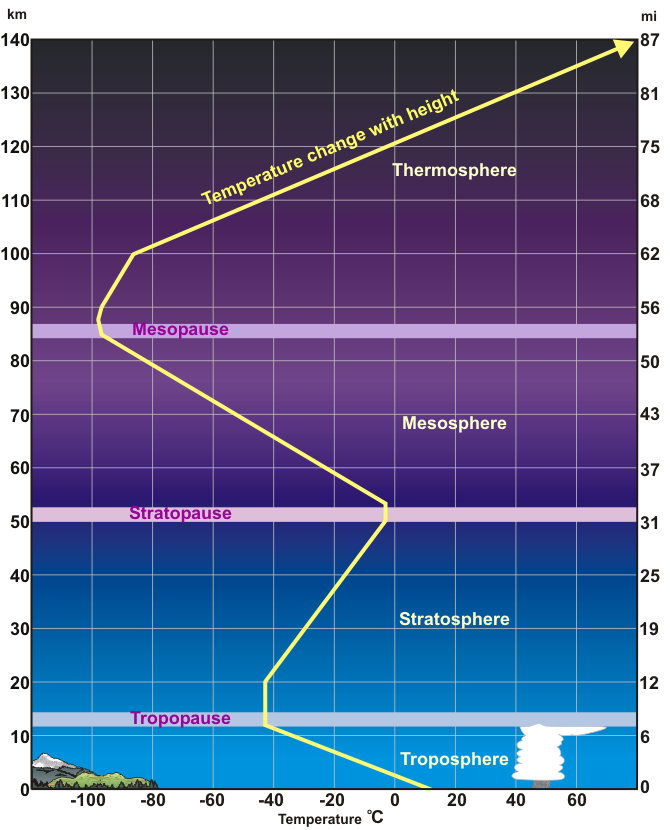
\includegraphics[width=.4\linewidth]{bilder/L6_atmos_layers.jpg}
    \caption{Layers in the atmosphere.}\label{fig:L6_atmos_layers}
\end{figure}

\subsection{Three cell global circulation pattern}
The three cell global circulation pattern is shown in \cref{fig:L6_three_cell_circulation}. The \emph{Hadley cell} can be found at \(0\)-\(\SI{30}{\degree}\). Here, air rises at equator resulting in that the upper air moves poleward. The Coriolis force then deflects the wind and it sinks at \(\pm\SI{30}{\degree}\). This process gives a belt of high surface pressure at \SI{30}{\degree}. The \emph{polar cell} can be found from \(60\)-\(\SI{90}{\degree}\). Cold, dense air descends at the pole which then cause high surface pressure. We get an equatorward flow near the surface, and deflection to the right due to Coriolis force. In between, from \(30\)-\(\SI{60}{\degree}\) we find the \emph{Ferrel cell}. The Ferrel cell is weak due to the lack of a strong heat source/sink, making air flows and temperatures highly variable.
\begin{figure}[t]
    \centering
    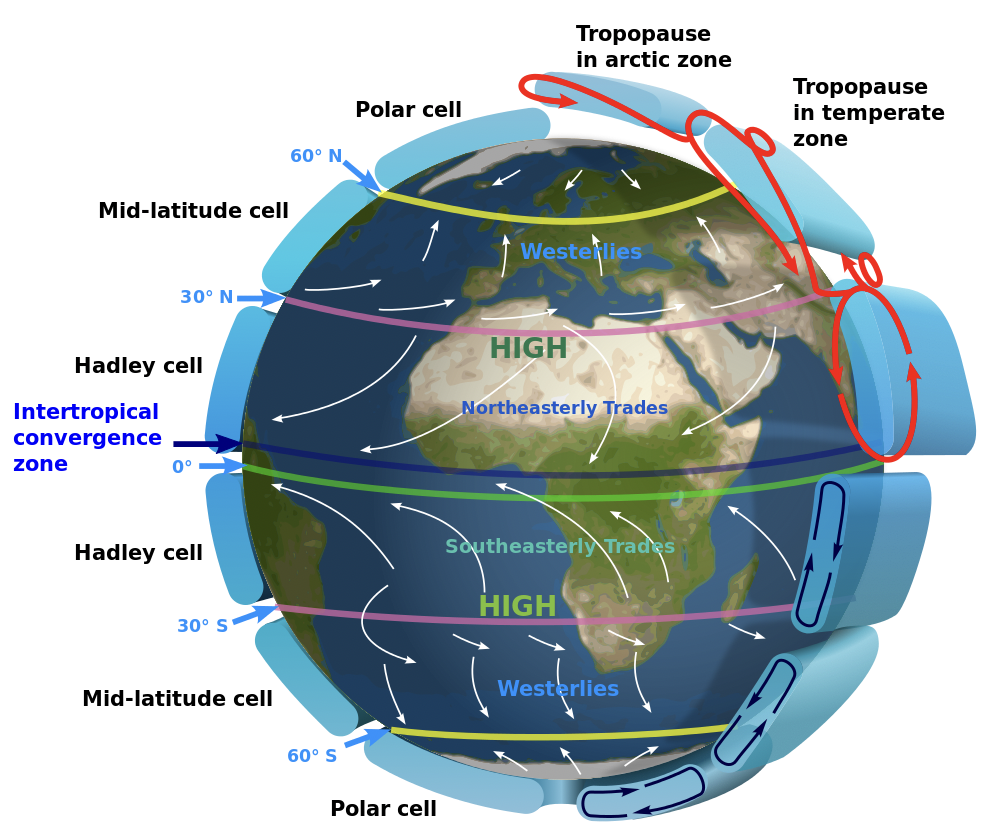
\includegraphics[width=.65\linewidth]{bilder/L6_three_cell_circulation.png}
    \caption{The three cell global circulation pattern.}\label{fig:L6_three_cell_circulation}
\end{figure}

\subsection{Stratospheric circulation}
\Cref{fig:L6_strat_circulation} show stratospheric circulation. The \emph{polar vortex} is a large area of low pressure (cyclone) formed in the upper troposphere and stratosphere. The pressure is stronger in the winter, and also stronger in the northern hemisphere. The \emph{polar night jet} lies on the border of the polar vortex. This is a strong westerly jet \(\sim \SI{100}{\metre/\second}\) centered around \SI{60}{\degree} latitude in the stratosphere and mesosphere during winter. It arises due to large temperature (and pressure) differences between equator and winter pole and the Coriolis effect. Warm air moves along the edge of the polar vortex, but cannot enter it. \emph{Summer easterlies} are zonal winds surrounding polar anticyclones in the stratosphere during summer. \emph{Stratospheric meridional circulation/Brewer-Dobson circulation} is meridional circulation from the tropics towards the poles in both hemispheres (stronger in winter) and this is driven by atmospheric waves. It is this circulation that is used to explain transport of ozone from tropical to polar latitudes. The last wind we consider is the \emph{quasi-biennial oscillation} (QBO). This has a 28--29-month cycle in zonal wind direction (between westerly and easterly) in the equatorial stratosphere, and it will mostly be within \SI{15}{\degree} latitude in each hemisphere.
\begin{figure}[t]
    \centering
    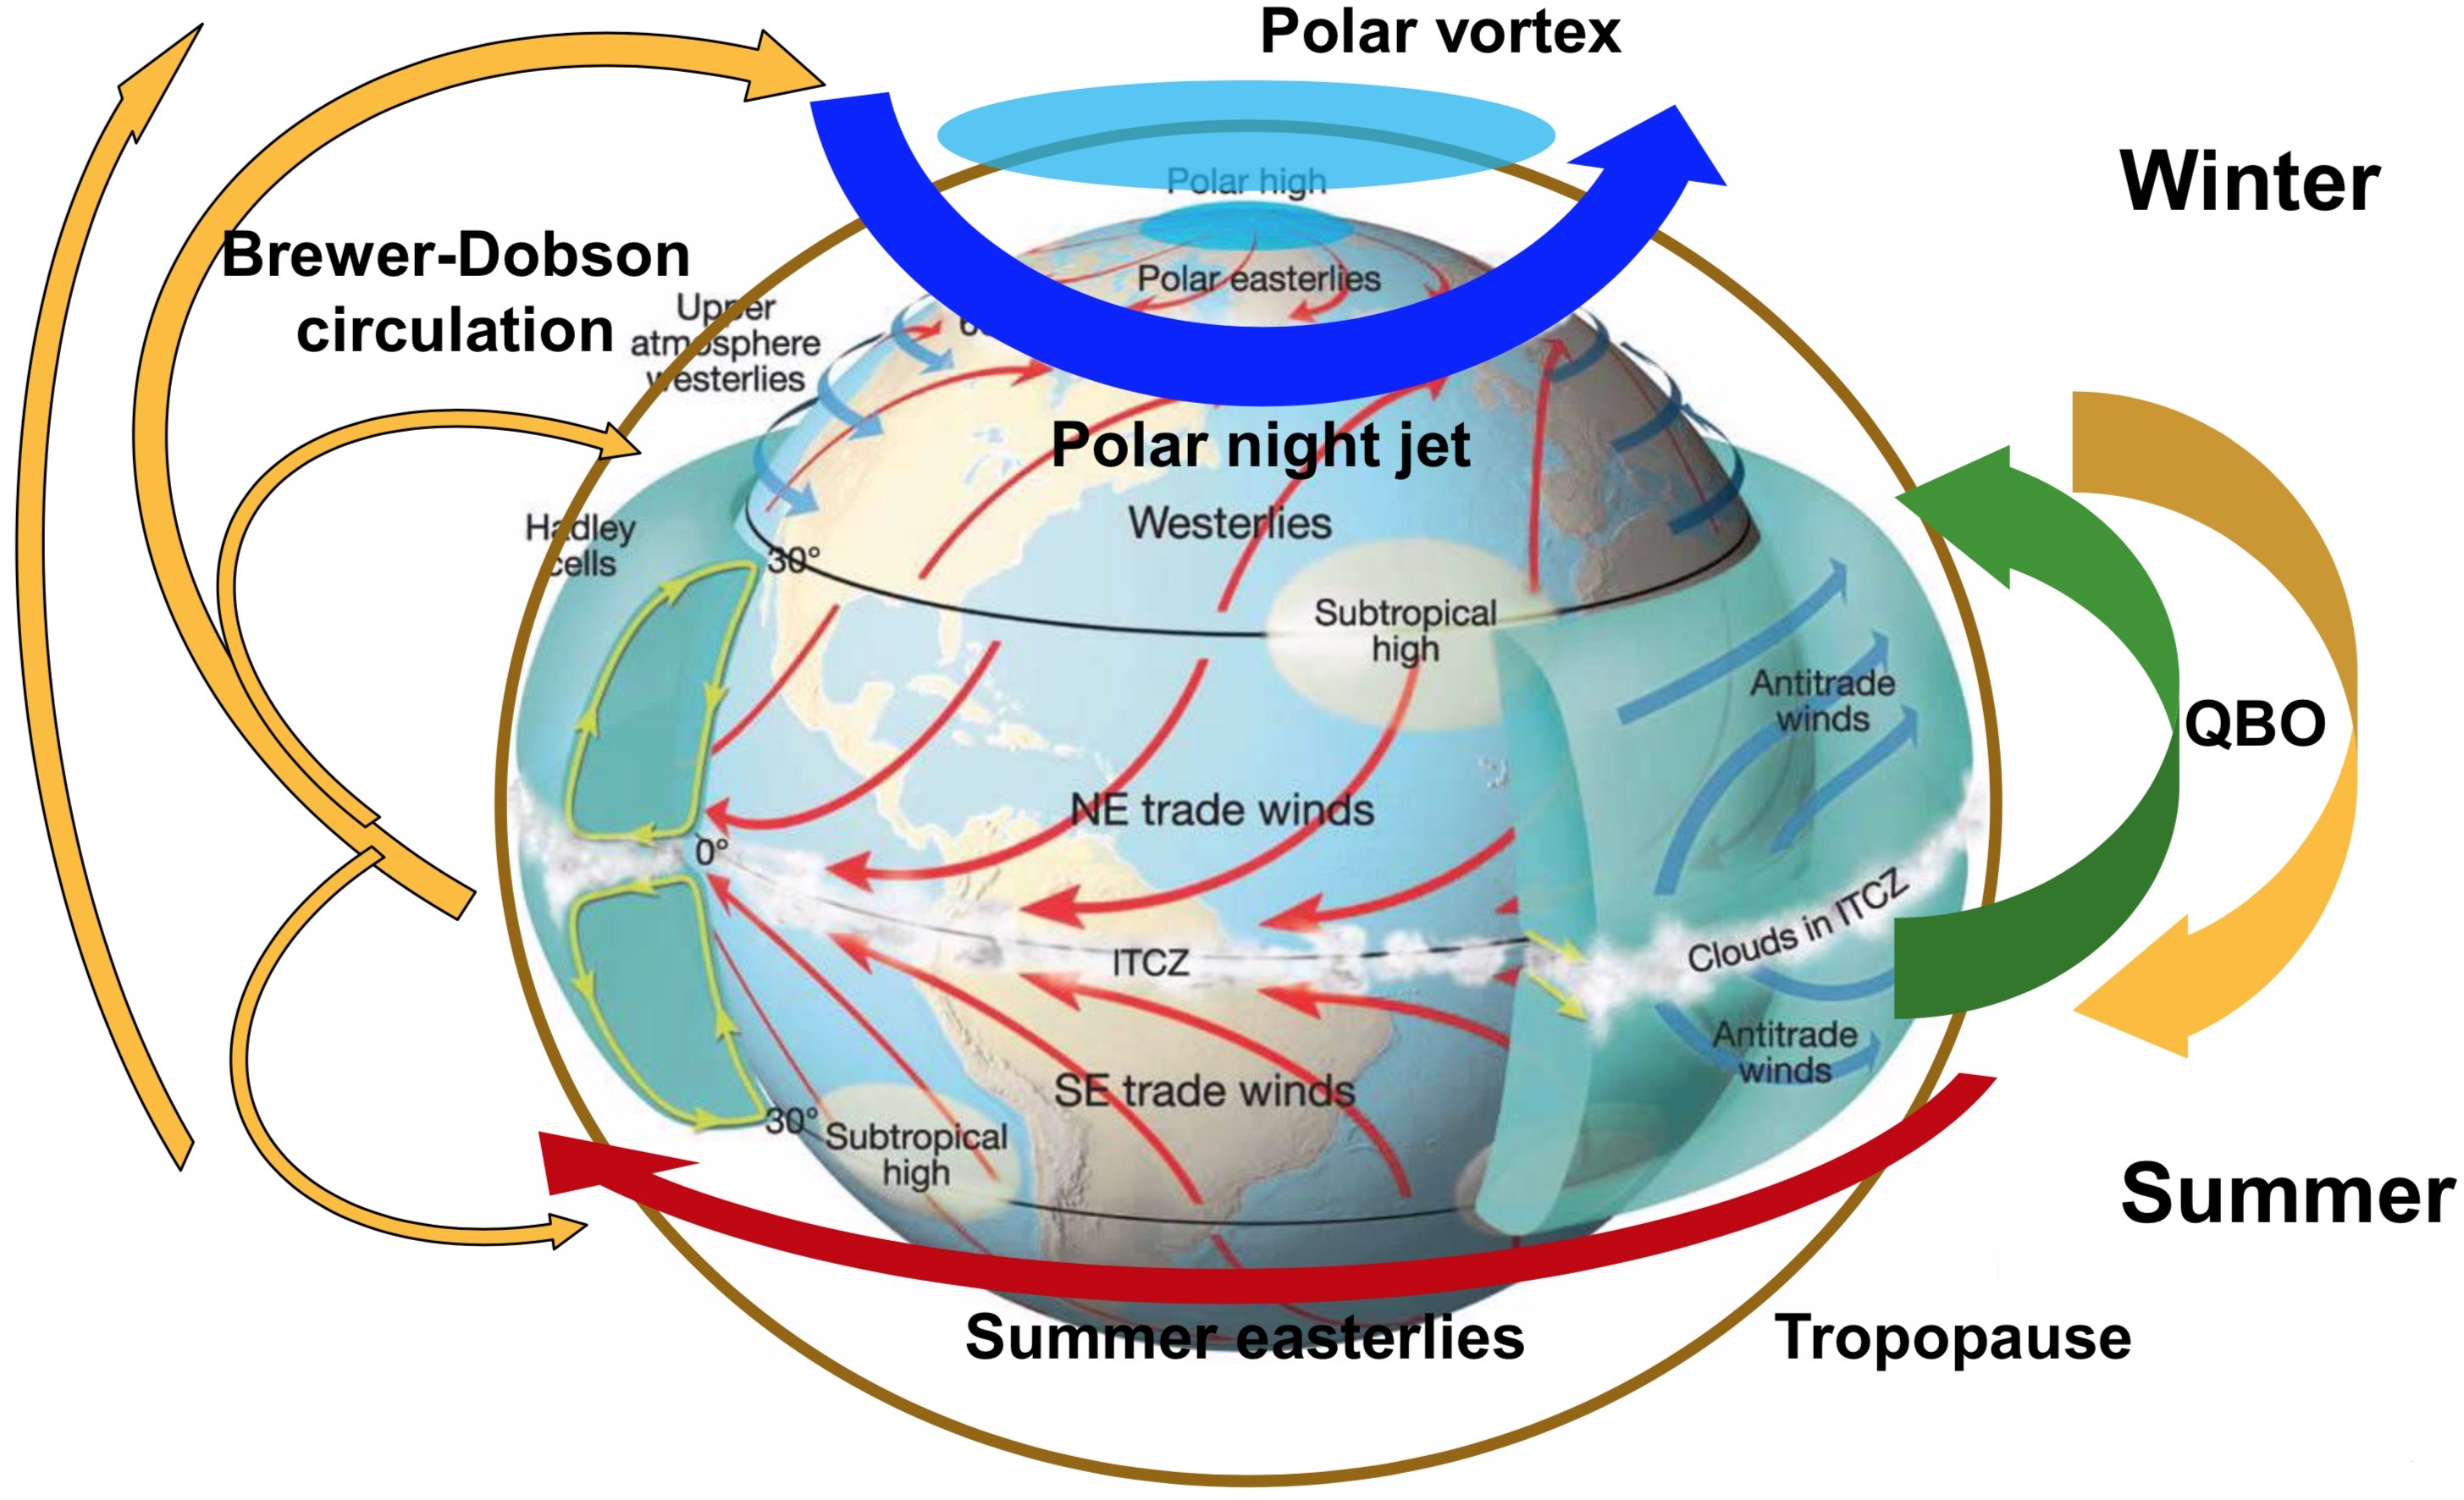
\includegraphics[width=.7\linewidth]{bilder/L6_strat_circulation.jpg}
    \caption{The stratospheric circulation pattern.}\label{fig:L6_strat_circulation}
\end{figure}

\subsection{Basic dynamics: waves}
We may classify waves by horizontal scale size, one being of planetary size (\(10^7\si{\metre}\)), e.g.\ Rossby waves and the other being of synoptic scale (\(10^6\si{\metre}\)), e.g.\ gravity waves.

Gravity wave breaking happen when GWs propagate upward in the layers. The amplitude grows and is proportional to \(\rho^{-1/2}\). At some altitude the amplitude becomes so large that non-linear effects become important and the mean flow can no longer support wave propagation. Wave breaking impacts on zonal mean winds and temperatures, and it drives the inter-hemisphere meridional circulation in the mesosphere (summer to winter hemisphere).

\section[Energetic particle precipitation \& the neutral atmosphere]{Effects of energetic particle precipitation on the neutral atmosphere \citep{NesseTyssoy2010Cium}}
\subsection{Ionization sources}
Sources for ionization are cosmic radiation, solar proton events (come in on open field lines, noticed in polar cap), auroral precipitation and relativistic electrons. \Cref{fig:L6_ionization_sources} show the ionization sources in the atmosphere.
\begin{figure}[t]
    \centering
    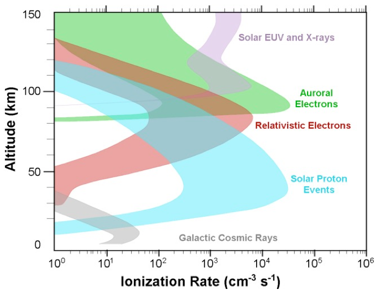
\includegraphics[width=.6\linewidth]{bilder/L6_ionization_sources.png}
    \caption{Ionization sources.}\label{fig:L6_ionization_sources}
\end{figure}

\subsubsection{Solar proton event}
\Cref{fig:L6_solar_proton_event} show how the proton flux changed during a solar proton event. From these events we get strong enhancement in energetic proton flux (\(>\SI{10}{\mega\electronvolt}\)), and damage to satellite electronics, radiation risk to astronauts and aircraft passengers/crew and HF radio wave absorption are among the effects we get from them, but they occur rarely (approx. 20/year at solar maximum, 0--3/year at solar min.). The events impact the whole polar cap and goes as far down as to the stratosphere. The effects it has on the atmosphere is well understood, and we have information about the flux. A proton flux measured by GOES-15, 1--16 September 2017 shows large enhancements in flux of high energy protons, and at Longyearbyen early on 5 September 2017 one could see loss of SuperDARN radar backscatter. At \url{https://umbra.nascom.nasa.gov/SEP/} you can find a list of such events.
\begin{figure}[t]
    \centering
    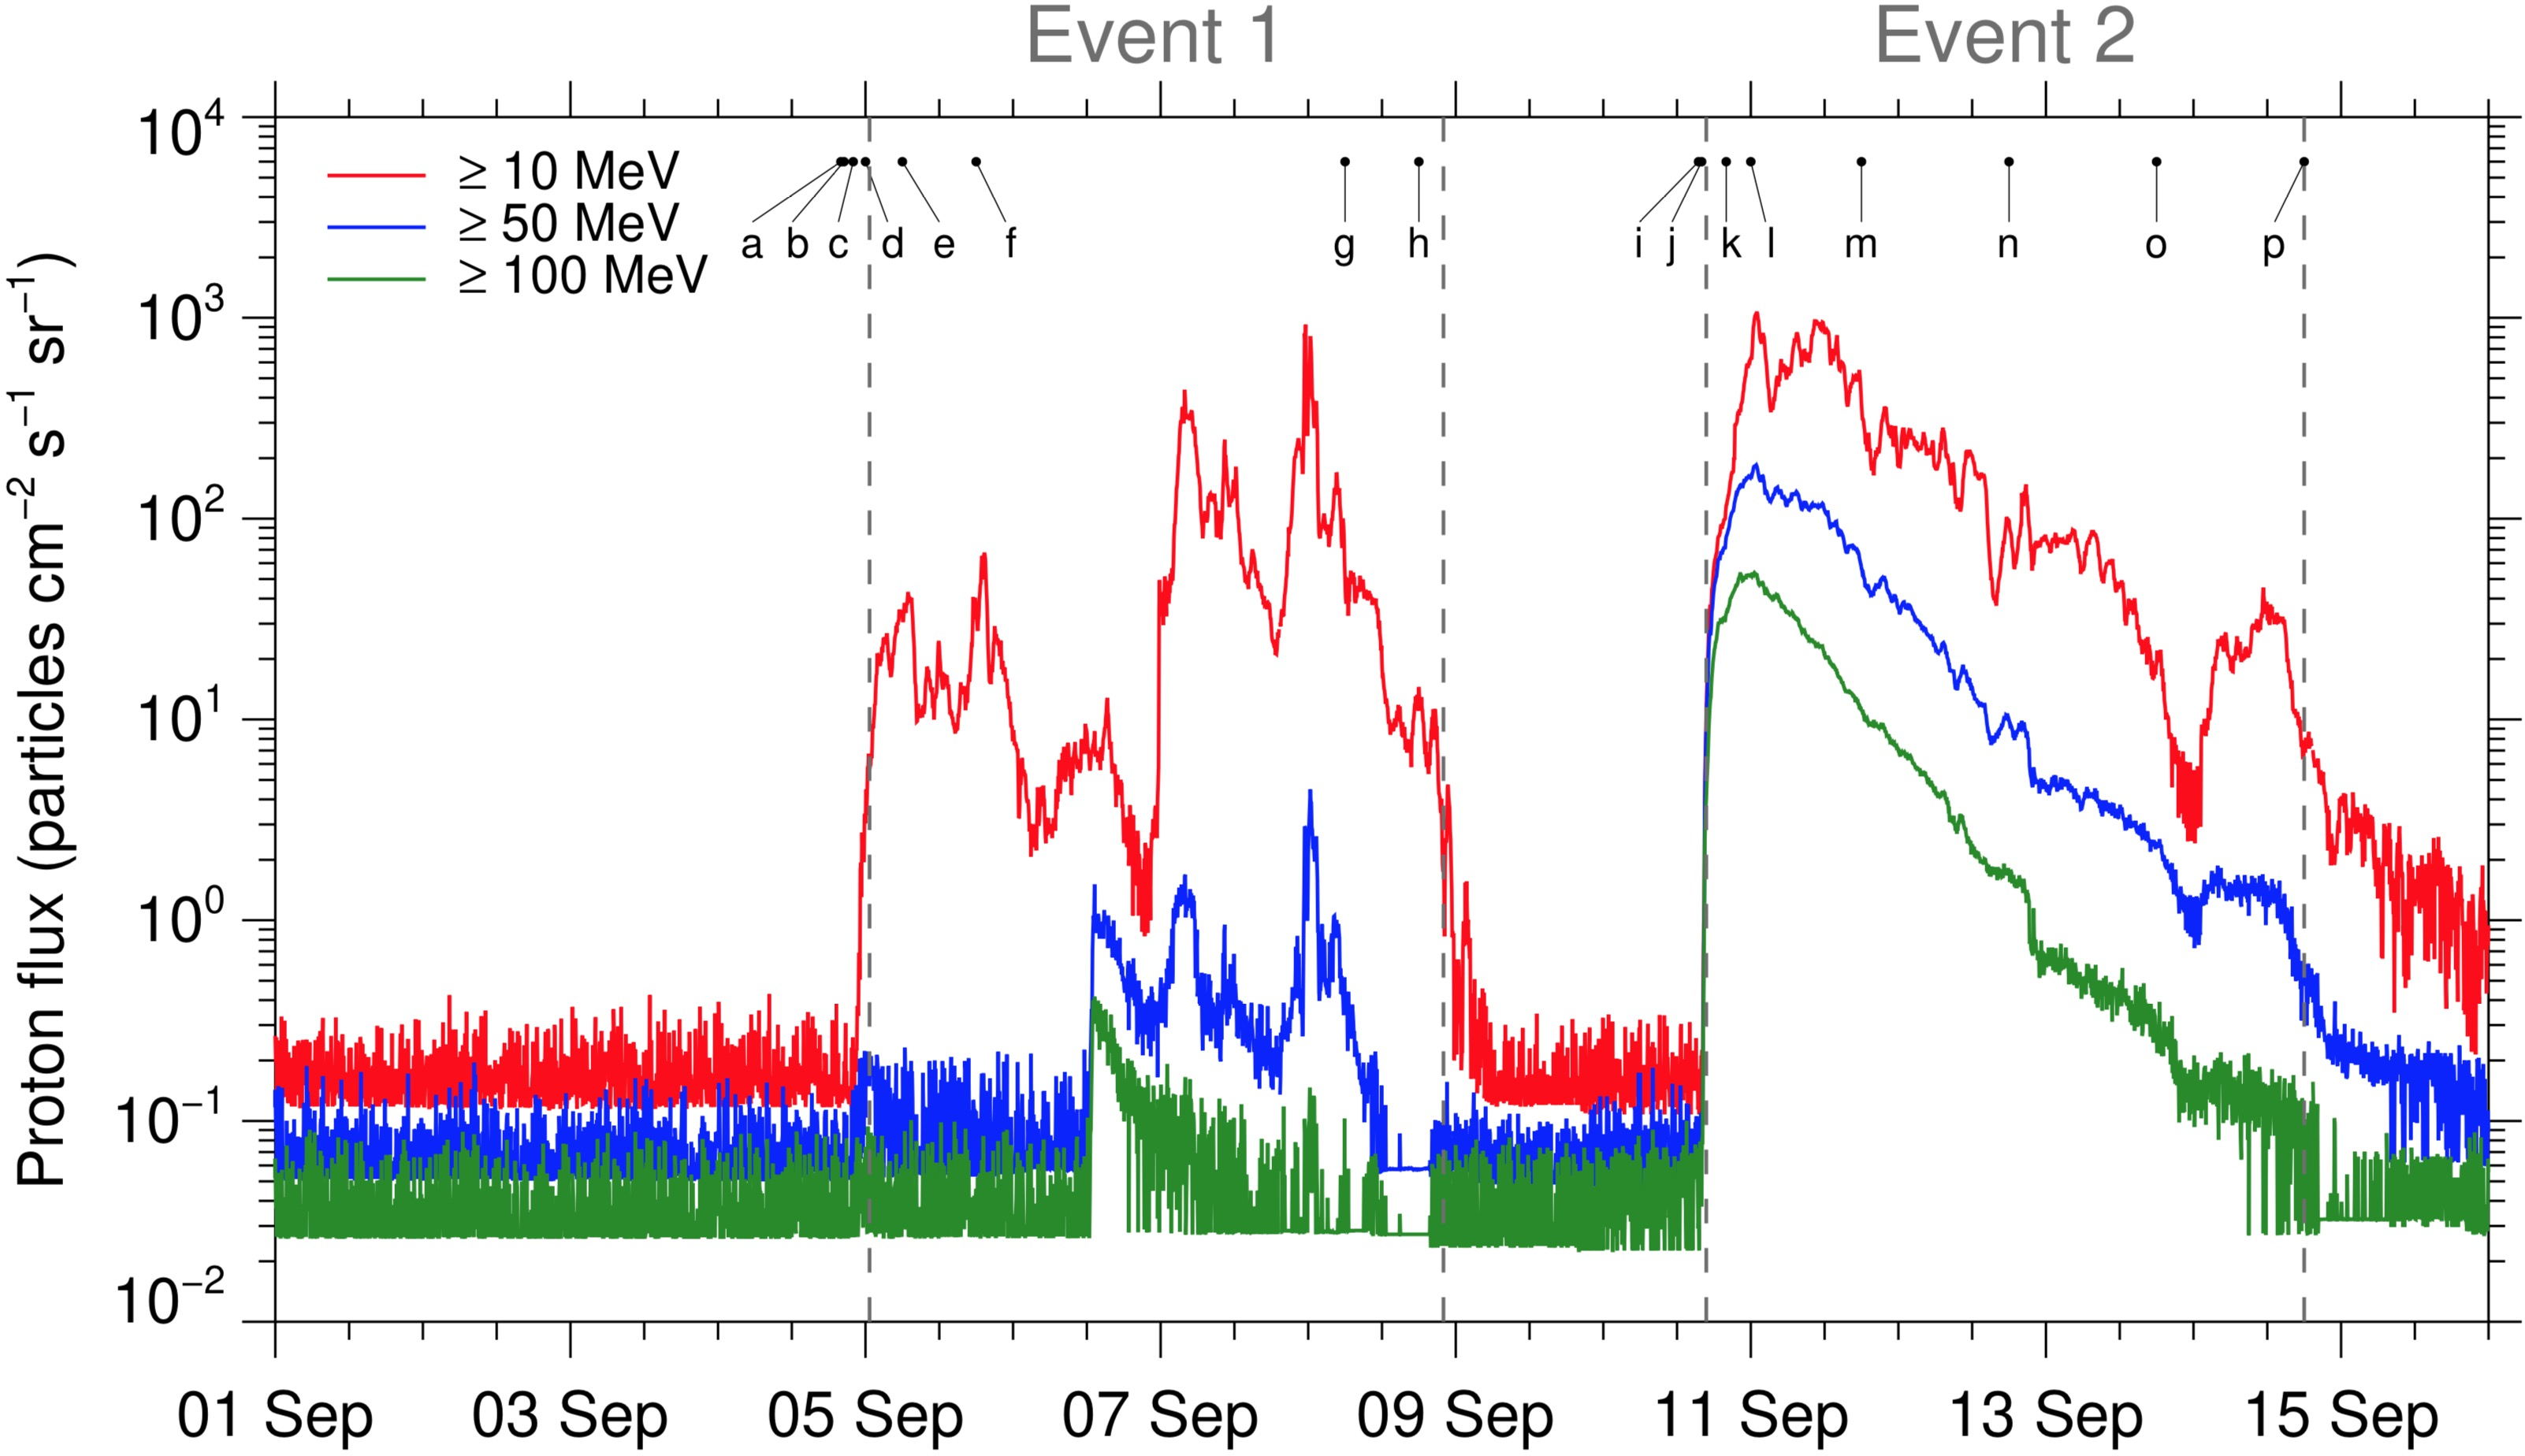
\includegraphics[width=.8\linewidth]{bilder/L6_solar_proton_event.jpg}
    \caption{Proton flux measured by GOES-15, 1--16 September 2017.}\label{fig:L6_solar_proton_event}
\end{figure}

\subsubsection{Electron precipitation}
Electron precipitation might give us relativistic electrons (\(\sim\SI{0.1}{\mega\electronvolt}\) to several \si{\mega\electronvolt}) during substorms and geomagnetic storms. When this is happening, we get auroral precipitation, including pulsating aurora. Compared to a solar proton event, electron precipitation is happening almost all the time, but impacts only the auroral oval.We do not have continuous observations of it and the effects on the atmosphere are not well understood. Auroral to relativistic energies are from \si{\kilo\electronvolt} to \si{\mega\electronvolt}, with pulsating aurora at keV level (electron precipitation).

The solar protons and the radiation belt electrons are a major source of ionization in the middle atmosphere.

The particle energy will determine the impact altitude. To produce \( 1 \) ion pair \si{\centi\metre^{-3}\second^{-1}} at \SI{60}{\kilo\metre} altitude (see \cref{fig:L6_impact_altitude}) we need
\begin{equation*}
    1\times\SI{20}{\mega\electronvolt}\tn{ protons } \si{\centi\metre^{-2}\second^{-1}}\quad\tn{or}\quad 100\times\SI{1}{\mega\electronvolt}\tn{ protons } \si{\centi\metre^{-2}\second^{-1}}
\end{equation*}
\begin{figure}[t]
    \centering
    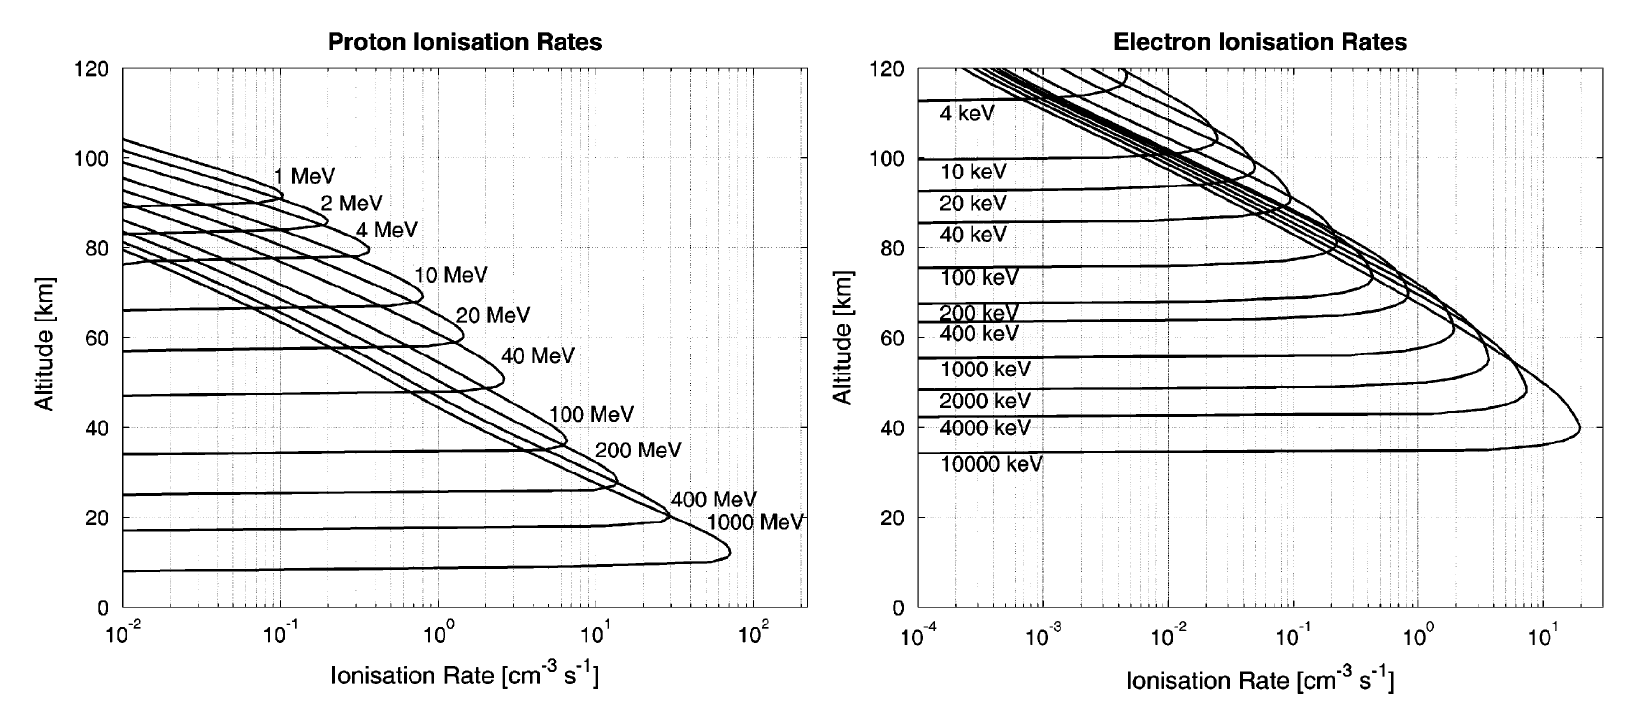
\includegraphics[width=.8\linewidth]{bilder/L6_impact_altitude.png}
    \caption{Altitude versus ionization rates for monoenergetic beams of protons (left) and electrons (right) \citep{TurunenEsa2009Iode}.}\label{fig:L6_impact_altitude}
\end{figure}
E-region ions are produced primarily by photoionization of molecular nitrogen and oxygen by UV radiation and X-rays, \(n_e\approx n_{\tn{O}_2^+}+n_{\tn{NO}^+}\). Positive ions in the D-region consists of a number of heavy cluster ions, e.g.~\(\tn{NO}^+\) and \(\tn{O}_2\). Negative ions in the D-region are density dependent, there is photo detachment, collisional detachment and ion-ion recombination.

But the chemically reactive ions have implications for the neutral atmosphere composition. Formation of \(\tn{HO}_{\tn{X}}\) and \(\tn{NO}_{\tn{X}}\) by positive ion chemistry give the possibility that they catalyze the ozone destruction. \(\tn{HO}_{\tn{X}}\) (\(\tn{H}+\tn{OH}+\tn{HO}_2\)) have a short lifetime while \(\tn{NO}_{\tn{X}}\) (\(\tn{N}+\tn{NO}+\tn{NO}_2\)) have longer chemical lifetime in the dark, hence especially in the winter period. Ozone is important for the energy budget through its role as a solar radiation absorber and radiator. \(\tn{HO}_{\tn{X}}\) contribute to a rapid but short-lived ozone loss in the mesosphere, while the \(\tn{NO}_{\tn{X}}\) could potentially influence both the mesospheric and stratospheric ozone balance.
\begin{align*}
    \tn{X}+\tn{O}_3&\rightarrow \tn{XO}+\tn{O}_2\\
    \tn{XO}+\tn{O}&\rightarrow \tn{X}+\tn{O}_2\\
    \tn{Net:}~\tn{O}+\tn{O}_3&\rightarrow 2\tn{O}_2
\end{align*}
Vertical downward transport is therefore mostly due to \(\tn{NO}_{\tn{X}}\), and also largely determined by the polar vortex.

\subsection{Consequences for atmospheric dynamics}
Chemical changes couple to wind and temperature changes and affect the energy transfer in the atmosphere. Energetic particle precipitation produces \(\tn{HO}_\tn{X}\) and \(\tn{NO}_\tn{X}\) which are catalysts for ozone destruction. More or less ozone give heating and cooling, i.e.\ temperature changes. This will then give winds which also has an impact on atmospheric waves (energy transfer). We then see that we have a dynamical amplification of initial impact. So we go from energetic particle precipitation (EPP) to increased winds in an indirect way (but not that long).

\section[Collisions between ions \& neutral particles]{Collisions between ions \& neutral particles (AB 2.13)}
Consider a gas consisting of two species, \(m\) and \(n\). These particles undergo collisions. Assume that the force per unit mass acting on the \(m\)-type particles due to collisions with \(n\)-type particles is proportional to the velocity difference between the two species, \(f_{m,n}\propto\gf{u}_m-\gf{u}_n\), with the force being given as
\begin{equation*}
    f_{m,n}=-\nu_{mn}\left(\gf{u}_m-\gf{u}_n\right)=\fracd{\gf{u}_m}
\end{equation*}
where \(f_{m,n}\) is the force (per unit mass) reducing \(\gf{u}_m\) due to collisions with \(n\)-type particle (\(u_m>u_n\)) and \(\nu_{mn}\) is the collision frequency. Momentum must be conserved, so
\begin{equation*}
    \rho_{m}f_{m,n}+\rho_{n}f_{n,m}=0
\end{equation*}
\coloredeq{eq:L6_collision_freq}{\therefore\rho_m\nu_{mn}\left(\gf{u}_m-\gf{u}_n\right)+\rho_n\nu_{nm}\left(\gf{u}_n-\gf{u}_m\right)=0}
So we can see that \(\rho_m\nu_{mn}=\rho_n\nu_{nm}\). For simplicity, consider only 1-dimensional motion. The equation of motion for \(m\)-type particles can be written as
\begin{equation*}
    \frac{\tn{d}u_m}{u_m-u_n}=-\nu_{mn}\tn{d}t
\end{equation*}
Using separation of variables we see, after integration, that this equation has the solution
\begin{equation*}
    u_m=u_m^0e^{-\nu_{mn}t}+u_n\left(1-e^{-\nu_{mn}t}\right)
\end{equation*}
where \(u_m\equiv u_m^0\) at \(t=0\). We get that \(\lim_{t\rightarrow\infty}u_m=u_n\) (equilibrium sol.\ for \(u_m\)). This occurs with characteristic relaxation time \(\tau_{m,n}=\frac{1}{\nu_{mn}}\). We can also write the equation of motion for \(n\)-type particles
\begin{equation*}
    u_n=u_n^0e^{-\nu_{nm}t}+u_m\left(1-e^{-\nu_{nm}t}\right)
\end{equation*}
with relaxation time
\begin{equation*}
    \tau_{nm}=\frac{1}{\nu_{nm}}=\frac{\rho_n}{\rho_m\nu_{mn}}=\frac{\rho_n}{\rho_m}\tau_{mn}
\end{equation*}
by using \cref{eq:L6_collision_freq}. What happens if \(\rho_m\gg\rho_n\)? Well, we have \(\tau_{mn}\gg\tau_{nm}\). This means that the \(n\)-type particles will reach equilibrium velocity \(\gf{u}_m\) much more quickly than the \(m\)-type particles will reach \(\gf{u}_n\). It also means that the \(n\)-type particles will ``feel'' the presence of the \(m\)-type particles more than the \(m\)-type will ``feel'' the \(n\)-type. I.e.\ we have \emph{drag} from one kind of particle to another.

The mean velocity is defined as
\begin{equation*}
    \widetilde{\gf{u}}:=\frac{\rho_{mn}\gf{u}_m+\rho_n\gf{u}_n}{\rho}
\end{equation*}
where \(\rho=\rho_m+\rho_n\). Since \(\fracd{\rho}=0\), we can write the momentum equation as
\begin{equation*}
    \rho\fracd{\widetilde{\gf{u}}}=-\left[\rho_m\nu_{mn}\left(\gf{u}_m-\gf{u}_n\right)+\rho_n\nu_{nm}\left(\gf{u}_n-\gf{u}_m\right)\right]=0
\end{equation*}
so the mean velocity is constant!
\begin{equation*}
    \gf{u}(\infty)=\gf{u}(t)=\gf{u}(0)
\end{equation*}

\section[Drag effects]{Drag effects (AB 2.15)}
Consider a simplified ionosphere with one neutral species and one ion species. These particles have velocities
\begin{equation*}
    \underset{\substack{\uparrow \\ \tn{ion}}}{\gf{v}_i}\quad\tn{and}\quad\underset{\substack{\uparrow \\\tn{neutral}}}{\gf{u}_n}
\end{equation*}
Assume that the neutral gas is in hydrostatic equilibrium, i.e.\ ignore vertical motion of neutrals. We consider three different cases. \boxed{\tn{Case 1}} (\Cref{fig:L6_no_init_neut_wind}). We here assume \(\gf{u}_{n0}=0\), i.e.\ no neutral wind and that the electric field is applied perpendicular to \(B\) so that
\begin{equation*}
    \gf{v}_{i0}=\frac{\gf{E}\times\gf{B}}{B^2}
\end{equation*}
The horizontal component of ion velocity will drag the neutrals along. Neutrals will also drag ions along which in turn does so \(\gf{v}_i\) will gain a component \(\vert\vert \) to \(\gf{B}\). We then get a stationary state when the ions and neutrals are moving horizontally at the same speed.
\begin{equation*}
    u_n=\frac{v_{i0}}{\sin(I)}=\frac{1}{\sin(I)}\frac{E}{B}
\end{equation*}
\boxed{\tn{Case 2}} (\Cref{fig:L6_no_init_ion_wind}). We now assume that \(\gf{v}_{i0}=0\), i.e.\ that ions initially are at rest meaning no \(E\)-field, and that we have horizontal neutral wind in the southward direction. The component of \(\gf{u}_n\) \(\vert\vert \) to \(\gf{B}\) will generate ion motion \(\vert\vert \) to \(\gf{B}\). The steady state ion velocity \(\gf{v}_i\) along the field is then given as
\begin{equation*}
    v_i=u_{n0}\cos(I)
\end{equation*}
or as
\begin{align*}
    &\tn{Horizontal component: } \hspace{-3cm}&v_{iH}&=u_{n0}\cos^2I&\\
    &\tn{Vertical component: } \hspace{-3cm}&v_{iV}&=u_{n0}\cos(I)\sin(I)&
\end{align*}
\boxed{\tn{Case 3}} (\Cref{fig:L6_diffusion_wind}). In our last case we again consider no initial neutral wind, \(u_{n0}=0\), and that plasma is diffusing downwards along the \(B\)-field lines at velocity \(v_{iD}\) (diffusion due to gravity + \(\nabla P\)). The ion motion has a horizontal component
\begin{equation*}
    v_{iH}=v_{iD}\cos(I)
\end{equation*}
This will drag the neutrals along until they attain horizontal velocity \(\gf{u}_n\). \(\gf{u}_n\) will produce an additional ion velocity along the field line, \(u_n\cos(I)\), and we get equilibrium when
\begin{align*}
    u_n=\left(v_{iD}+u_n\cos(I)\right)\cos(I)\\
    \Rightarrow u_n=\frac{v_{iD}\cos(I)}{\sin^2(I)}
\end{align*}
The final plasma velocity \(\vert\vert \) to \(B\) is
\begin{equation*}
    v_i=\frac{v_{iD}}{\sin^2(I)}
\end{equation*}
\begin{figure}[t]
    \centering

    \begin{subfigure}[t]{.32\linewidth}
        \centering
        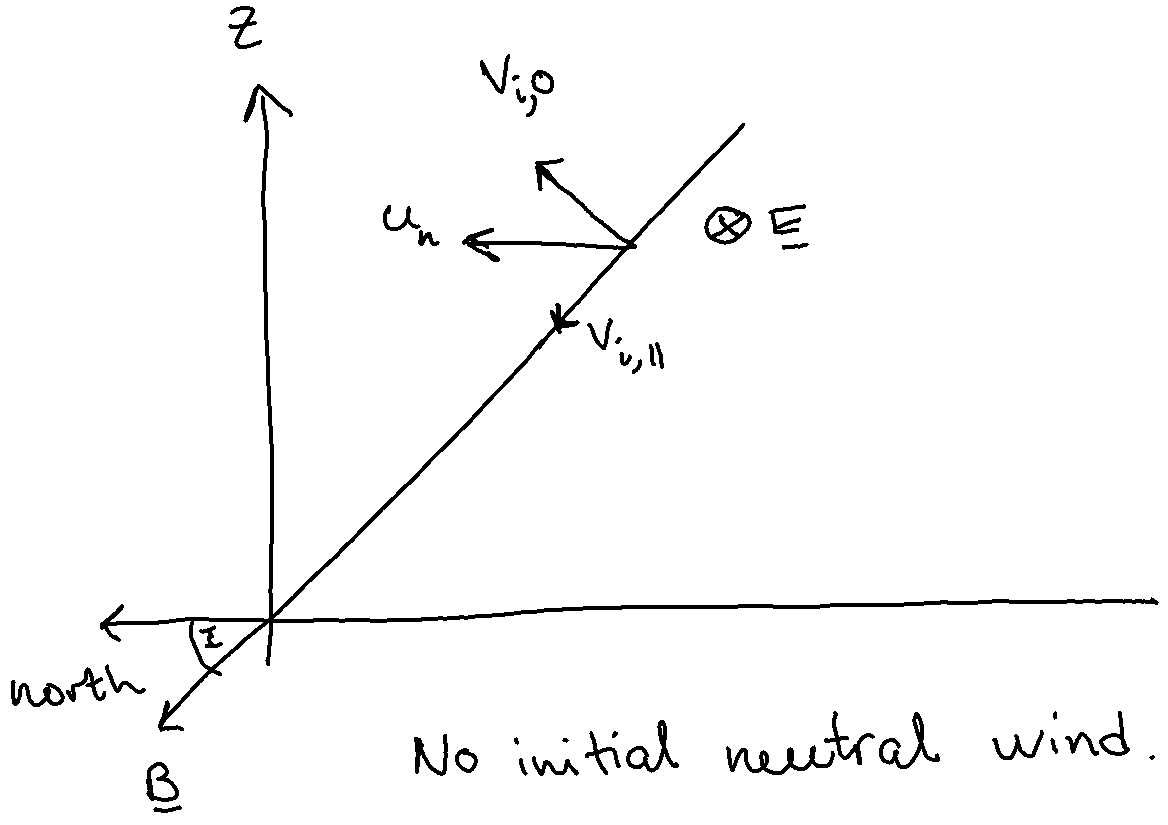
\includegraphics[width=\linewidth]{bilder/L6_no_init_neut_wind.png}
        \caption{}\label{fig:L6_no_init_neut_wind}
    \end{subfigure}
    \begin{subfigure}[t]{.32\linewidth}
        \centering
        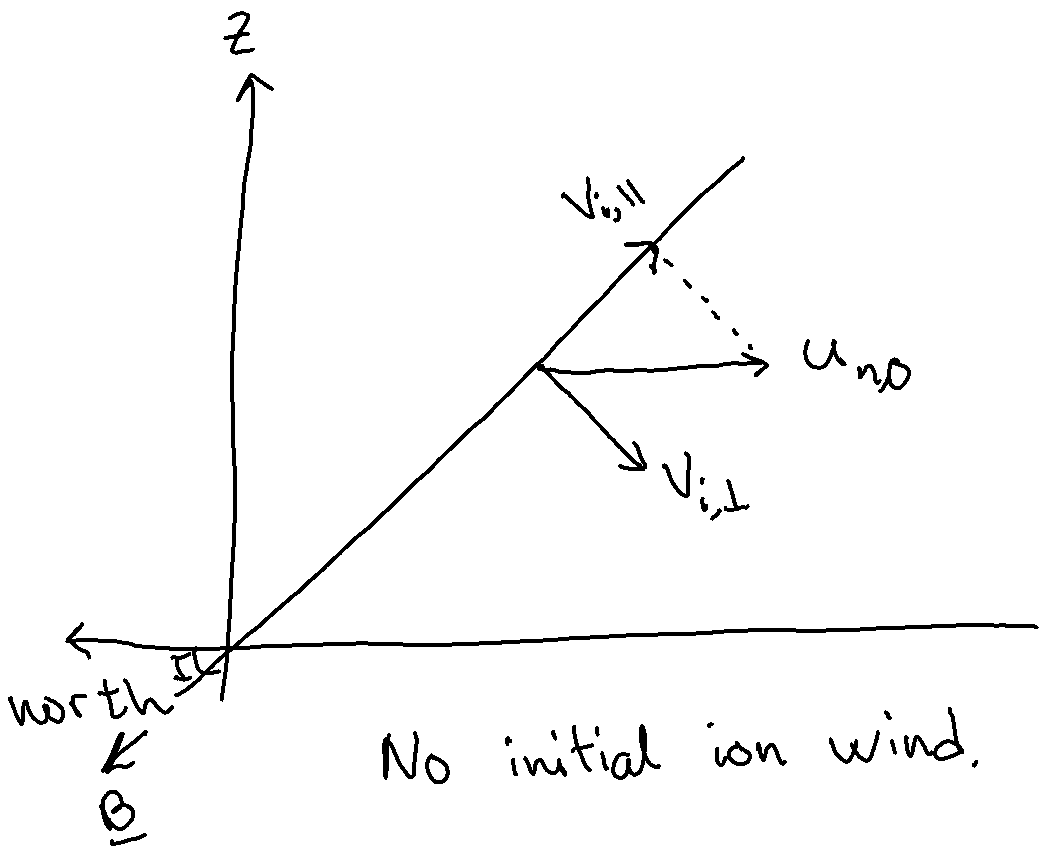
\includegraphics[width=\linewidth]{bilder/L6_no_init_ion_wind.png}
        \caption{}\label{fig:L6_no_init_ion_wind}
    \end{subfigure}
    \begin{subfigure}[t]{.32\linewidth}
        \centering
        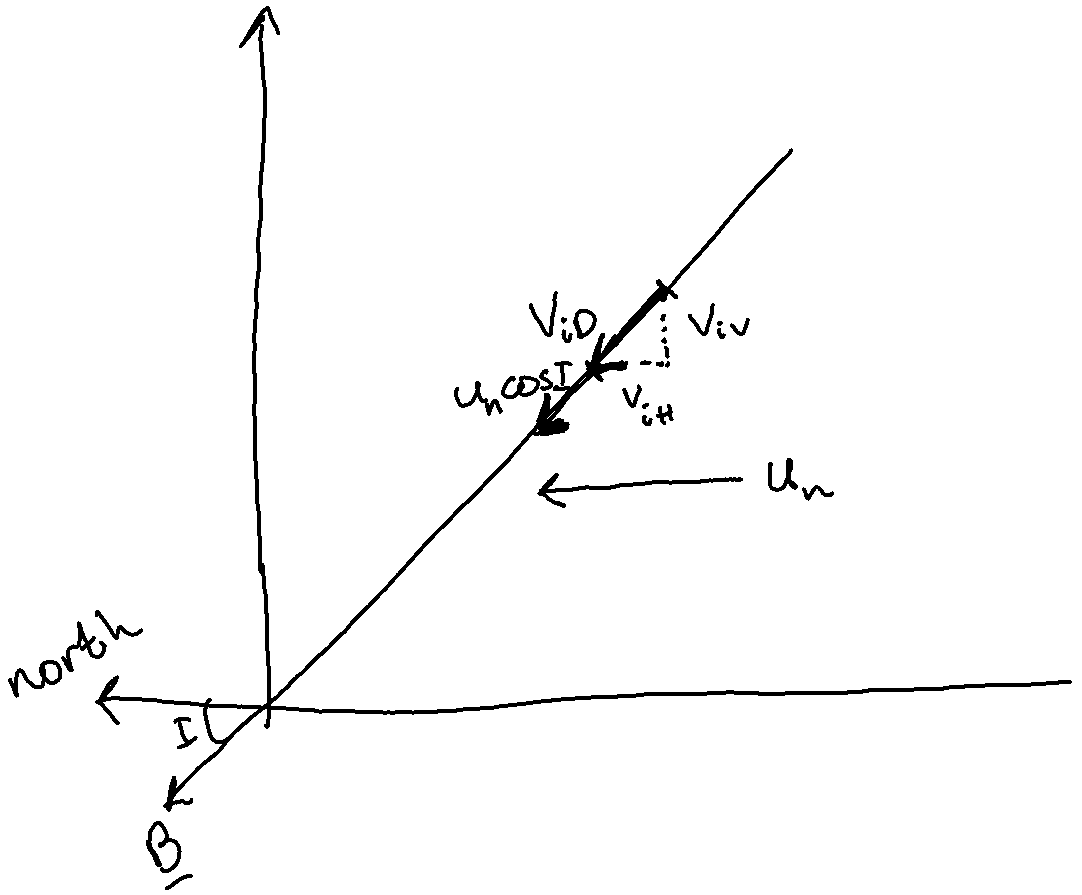
\includegraphics[width=\linewidth]{bilder/L6_diffusion_wind.png}
        \caption{}\label{fig:L6_diffusion_wind}
    \end{subfigure}

    \caption{\subref{fig:L6_no_init_neut_wind}: No initial neutral wind. \subref{fig:L6_no_init_ion_wind}: No initial ion wind. \subref{fig:L6_diffusion_wind}: Diffusion effect on ion wind.}\label{fig:L6_ion_and_neutral_winds}
\end{figure}

\section[Thermospheric neutral wind]{Thermospheric neutral wind (AB 2.16, 2.17 \& 2.18)}
During daytime, we get an expansion of the atmosphere called the diurnal bulge. The temperature distribution creates large-scale pressure gradients which again creates winds. In general we get velocities directed from the dayside across the pole to the nightside and the wind speeds can be of \(\sim\SI{40}{\metre\second^{-1}}\) directed approximately perpendicular to the isotherms
\begin{figure}[t]
    \centering
    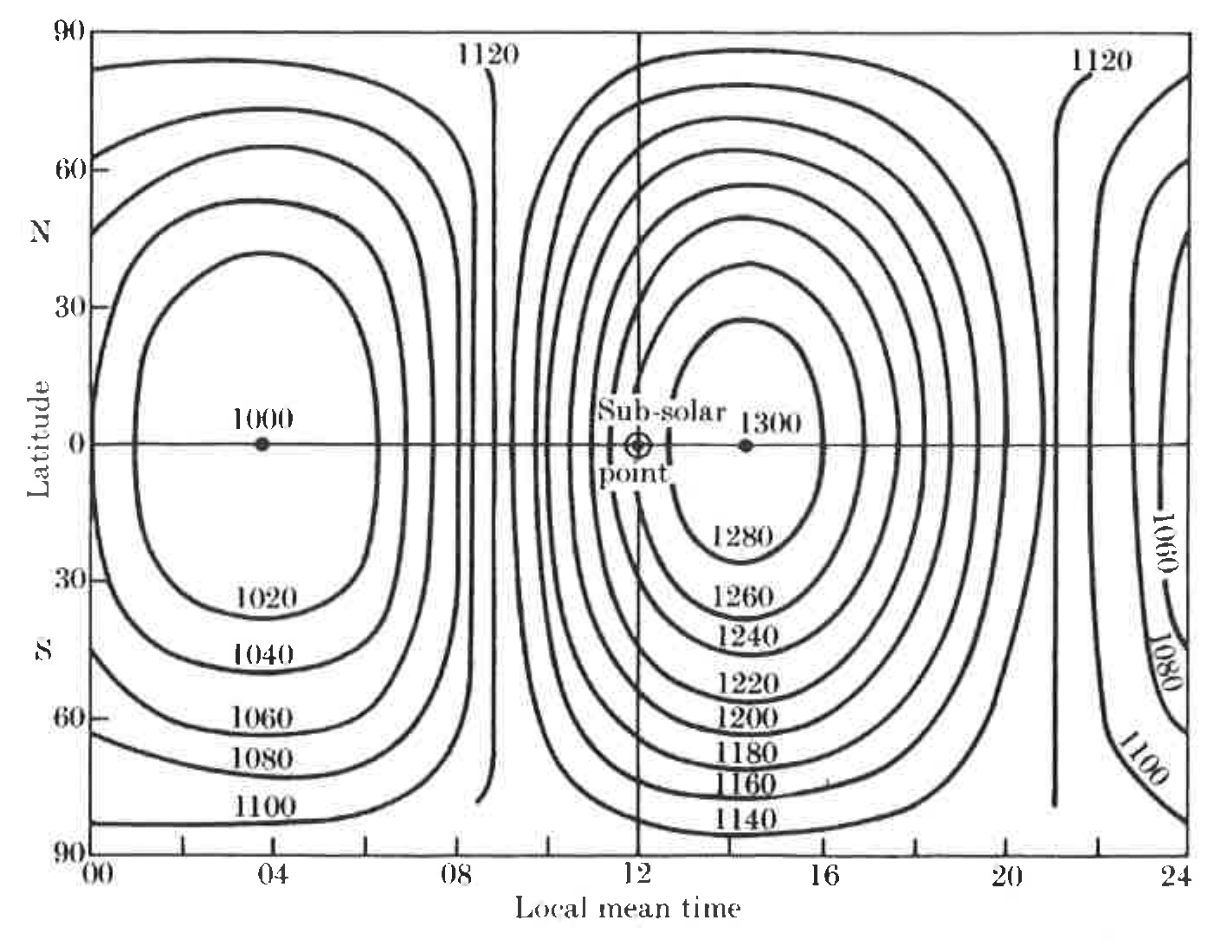
\includegraphics[width=.6\linewidth]{bilder/L6_winds_diurnal.png}
    \caption{Modelled isotherms at the thermopause, \(\sim\SI{400}{\kilo\metre}\) altitude.}\label{fig:L6_winds_diurnal}
\end{figure}
The equation of motion for a neutral gas can be expressed as
\begin{equation*}
    \fracd{\gf{u}}=-\frac{1}{\rho}\nabla p+\gf{g}+\gf{f}
\end{equation*}
We ignore all terms except the pressure gradient force and \(\gf{f}\). A steady state solution for the neutral wind is
\begin{equation*}
    \gf{f}=\frac{1}{\rho}\nabla p
\end{equation*}
If we assume \(\gf{f}\) to only be caused by collisions between neutrals and ions (\(\gf{f}=-\nu_{ni}(\gf{u}_n-\gf{v}_i)\)) and that we have an ideal gas, the velocities will be
\begin{equation*}
    \gf{u}_n=-\frac{1}{\rho\nu_{ni}}\nabla p+\gf{v}_i=-\frac{k}{\rho\nu_{ni}}\nabla T+\gf{v}_i
\end{equation*}
If \(\gf{v}_i\) is negligible and there are no horizontal variations in the neutral density, the neutral wind will blow along the temperature gradients. A more realistic version of the equation of motion for a neutral gas would be
\begin{equation*}
    \p{t}{\gf{u}_n}=-\left(\gf{u}_n\cdot\nabla\right)\gf{u}_n-2\Omega\times\gf{u}_n+\gf{g}-\frac{1}{\rho}\nabla p-\nabla\psi+\frac{\mu}{\rho}\nabla^2\gf{u}_n-\nu_{ni}\left(\gf{u}_n-\gf{v}_i\right)
\end{equation*}
where \(\Omega \) is the angular velocity of the Earth, \(\psi \) is the potential due to centrifugal and tidal forces and \(\mu \) is the coefficient of viscosity. The equation of motion for ions is
\begin{equation*}
    m_i\p{t}{\gf{v}_i}=-m_i\left(\gf{v}_i\cdot\nabla\right)\gf{v}_i+q\left(\gf{E}+\gf{v}_i\times\gf{B}\right)-m_i\nu_{in}\left(\gf{v}_i-\gf{u}_n\right)
\end{equation*}
where \(m_i\) is the ion mass (\(m_i\gg m_e\)). Here, we ignore Coriolis force, gravity, pressure forces, centrifugal and tidal forces, and viscosity. In the F-region, \(\gf{u}_n\) is controlled mostly by the pressure and ion drag terms, while in the E-region the velocity is controlled mostly by pressure and the Coriolis terms.

\section{Worksheet: Analyzing~\citet{NesseTyssoy2010Cium}}
\begin{longtabu} to \textwidth { | X[l] | X[l] | }
    \hline
    \multicolumn{2}{|l|}{\cellcolor{black!20}\textbf{1. Purpose/hypothesis/aim of the study}}\\
    \hline
    Write down the exact statement in which the authors describe what they were testing. &  A statistical evaluation on the upper mesospheric \& lower thermosphere temperature effect caused by energetic particle precipitation. \vspace{2mm}\\
    \hline
    Describe the purpose of the study (as you understand it) in your own words. & They want to find out if there is significant heating in the upper mesosphere \& lower thermosphere due to precipitation of energetic particles. \vspace{2mm}\\
    \hline
    What was the ``gap'' in the research that the authors were trying to fill by doing this study? & The energy budget done using a large amount of data instead of case studies. \vspace{2mm}\\
    \hline
    \multicolumn{2}{|l|}{\cellcolor{black!20}\textbf{2. Major findings of the study}}\\
    \hline
    Write down or highlight the passages in the article where the authors give their \underline{major} findings/conclusions. \vspace{2mm}& Ok. \\
    \hline
    Write 2--3 ``key points'' summarizing the main findings/conclusions of the study in your own words (about 100 characters per key point). & They found that the temperatures seemed to reach a state of equilibrium as the flux of the energetic particles increased. When sorting based on the Kp values, they got way bigger temperature differences in the region above \SI{100}{\kilo\metre}. Below this altitude, there was no apparent accumulated temperature trend. \vspace{2mm}\\
    \hline
    \multicolumn{2}{|l|}{\cellcolor{black!20}\textbf{3. How did the authors test their hypothesis?}}\\
    \hline
    Describe the method used to measure the temperatures in this study. Over what altitude range can this method be used? What is the spatial resolution of the temperature data? & They used the satellites TIMED and NOAA 15, 16 and 17 which has the instruments SABER and MEPED on, respectively. SABER measures up to about \SI{130}{\kilo\metre} with a vertical resolution of \SI{2}{\kilo\metre}. MEDPED looks at the altitude range \SI{90}{\kilo\metre}--\SI{140}{\kilo\metre}. \vspace{2mm}\\
    \hline
    Which detector angle (\SI{9}{\degree} or \SI{89}{\degree}) on MEPED is most important for this study and why? What is meant by the ``loss cone''? & The vertical detector angle is the most important, since it is looking in the direction where particles are lost into the atmosphere, i.e.\ the precipitating particles. The ``loss cone'' is describing the particles that have enough energy to escape the magnetic field of the Earth, instead of oscillation in the van-Allen belts. \vspace{2mm}\\
    \hline
    Briefly summarize the main steps that the authors use to process/organize the data. Try to explain in your own words as much as possible. & They collected data from two different one-month periods, and made averages based on these two intervals. Afterwards, they also split the data from the October/November period into above 4 Kp and below/equal to 4 Kp, and made averages of those two groups of data to compare. They also differentiated between the different energies of the particles, making four different averages for each interval (three energy regions for protons, one for electrons). \vspace{2mm}\\
    \hline
    Do the authors suggest any problems or limitations with their methodology? Do \underline{you} se any problems or limitations with their methodology? & They discuss if Joule heating, which plays a more significant role during quiet conditions in summer, might make the effect of precipitation harder to see in the May/June interval. Only certain times a day. \vspace{2mm}\\
    \hline
    \multicolumn{2}{|l|}{\cellcolor{black!20}\textbf{4. Results}}\\
    \hline
    Describe the observed temperature changes in the \underline{lower thermosphere} during both intervals. What processes might account for the different temperature responses during these two intervals? & It is increasing in the fall interval, but not significantly in the summer. Larger substorms might be the reason for the big difference, and also Joule heating which plays a smaller role in the fall compared to summer. Higher Pedersen conductivity. \vspace{2mm}\\
    \hline
    Describe the observed temperature changes in the \underline{upper mesosphere}. Why is it difficult to determine the effects of particle precipitation on temperature in the upper mesosphere? What steps do the authors take to extract any temperature trends that are not apparent in Figures 2 \& 4? & The upper mesosphere have little change in any of the two intervals, also for large Kp value. They sort, as mentioned, into high/low Kp in Figure 6 which they do not in Figures 2 \& 4, but still no trend can be found. They mention that a paper from Pancheva et al. [2007] did see a difference, but that it was based on ground-based observations associated with a specific region and local time. They go on to say that they should investigate whether there are any apparent local time of geomagnetic latitude dependencies in the temperature responses. \vspace{2mm}\\
    \hline
    What physical process might cause cooling of the upper mesosphere in response to particle precipitation? \vspace{2mm}& Increased \(\tn{CO}_2\) levels, infrared radiation. \\
    \hline
    \multicolumn{2}{|l|}{\cellcolor{black!20}\textbf{5. Evaluation}}\\
    \hline
    Do the authors suggest any problems or limitations with the study that could lead to unreliable results? \vspace{2mm}& Maybe the precipitation to temperature was too close in time? Do ozone play a significant role? \\
    \hline
    Do the authors' conclusions make sense to you? Are the conclusions too broad or too narrow based on what was actually done in the study? & It makes sense, they do not for example make any conclusions about whats happening below \SI{100}{\kilo\metre}. Kp value might also be a bit too bad as a value of sorting the data. They are self critical and hence I feel they are neither too broad or too narrow. \vspace{2mm}\\
    \hline
    Write (in your own words) the significant contributions of the experimental work in this journal article as reported by the authors. \vspace{2mm}& The statistical approach they make to bring in big data to investigate the energy budget. \\
    \hline
\end{longtabu}



\chapter{Revisit: Pulsations \& MHD-waves}
\begin{remark}
    Section made from lectures done by Jøran Moen. Other sources are \citet{1995Itsp} --- chapter 11.
\end{remark}
\noindent\textbf{This week:}
\begin{enumerate}[\(\bullet \)]
    \item guess harmonic oscillations
    \item derive dispersion relation
    \item identify wave modes\begin{enumerate}[\(\triangleright \)]
        \item plasma acoustic
        \item Alfvén
        \item magnetosonic
    \end{enumerate}
    \item energy sources
\end{enumerate}
\section{MHD-equations: introduction}
The MHD-waves are ULF waves, i.e.~\(f<f_p,f_{ci}\), where
\begin{equation*}
    f_p=\frac{1}{2\pi}\sqrt{\frac{ne^2}{\epsilon_0m}},\quad f_{ci}=\frac{1}{2\pi}\frac{qB}{m}
\end{equation*}
is the plasma and ion gyro frequencies respectively. We remind ourself of the MHD equations, \cref{eq:MHD_1,eq:MHD_2,eq:MHD_3,eq:MHD_4,eq:MHD_5,eq:MHD_6}. From these six, we may combine them to reduce the number of equations to five. We then end up with
\begin{align}
    \p{t}{\rho}+\nabla\cdot\left(\rho \gf{v}\right)&=0\label{eq:simple_MHD1}\\
    \rho\left[\p{t}{\gf{v}}+(\gf{v}\cdot\nabla)\gf{v}\right]&=-\nabla p-\frac{1}{\mu_0}\gf{B}\times\left(\nabla\times\gf{B}\right)\label{eq:simple_MHD2}\\
    \p{t}{\gf{B}}&=\nabla\times\left(\gf{v}\times\gf{B}\right)\label{eq:simple_MHD3}\\
    \nabla\cdot\gf{B}&=0\label{eq:simple_MHD4}\\
    p&=S\rho^\gamma\label{eq:simple_MHD5}
\end{align}
where \(S\) is the entropy and we have assumed frozen in conditions where \(\gf{E}\) can be written into \(\gf{v}\times\gf{B}\). We then linearize these equations by writing all parameters on the form \(\xi=\xi_0+\xi_1\) and only keeping terms of \(\orderof(1)\) or less. We want to rewrite the latter equation by finding the gradient, which gives
\begin{equation}\label{eq:simplify_MHD6}
    \begin{aligned}
        \nabla p_1&=S\gamma{\left(\rho_0+\rho_1\right)}^{\gamma-1}\nabla\rho_1\\
        &=\gamma\frac{p_0+p_1}{\rho_0+\rho_1}\nabla\rho_1,\quad p_0\gg p_1, \rho_0\gg\rho_1\\
        &=\gamma\frac{p_0}{\rho_0}\nabla\rho_1=c_s^2\nabla\rho_1
    \end{aligned}
\end{equation}
where we have used that \(S=\left(p_0+p_1\right)/{\left(\rho_0+\rho_1\right)}^\gamma \). We assume normal mode solutions, i.e.\ we write \(\xi_1=\widetilde{\xi}e^{i\left(\gf{k}\cdot\gf{r}-\omega t\right)}\), where \(\xi_1\) may be either a scalar or a vector.

\section{Acoustic wave}
We can reduce our five equations even further by choosing to neglect both the electric and the magnetic field, leaving only the top two equations. We use the result from \cref{eq:simplify_MHD6} and plug it into \cref{eq:simple_MHD2}, and then replace all parameters with normal mode solutions. Doing all this yields
\begin{align*}
    -i\omega\rho_1+\rho_0i\gf{k}\cdot\gf{u}_1=0\\
    i\omega\rho_0\gf{u}_1=-i\gf{k}c_s^2\rho_1
\end{align*}
From here, we can find the dispersion relation we were looking for, given as
\begin{equation*}
    \omega^2=k_x^2C_s^2
\end{equation*}
where we have defined \(\gf{k}=k_x\f{x}\) and \(C_s\) is the phase velocity.

\section{Waves in cold plasma}
We now write the pressure as
\begin{align*}
    p&=n_{i}k_{B}T_i+n_{e}k_{B}T_e\\
    p_B&=\frac{B^2}{2\mu_0}
\end{align*}
where \(p_B\) is the magnetic pressure. If the magnetic field dominate the pressure, we express this with the parameter
\begin{equation*}
    \beta=\frac{p}{p_B}=\frac{p}{B^2/2\mu_0}\ll 1
\end{equation*}
The MHD equations for a cold plasma is as given in \cref{eq:simple_MHD1,eq:simple_MHD2,eq:simple_MHD3,eq:simple_MHD4,eq:simple_MHD5}, but where \(\nabla p\rightarrow 0\), i.e.\ \cref{eq:simple_MHD1,eq:simple_MHD2,eq:simple_MHD3} are the relevant equations.

\section{Exercises}
\begin{enumerate}
    \item [\textbf{EXERCISE 1 --- Exam 2004}]~\vspace{1pt}\begin{enumerate}[(a)]
        \item Assume a static uniform magnetic field oriented along the \(y\)-axis with a static electric field along the \(z\)-axis. Define your coordinate system and sketch the particle trajectories separately for electrons and ions. Clearly indicate the direction of movement.
        \mylinbrk{}
        The movement is illustrated in \cref{fig:L7_ExB}.
        \item Assume a magnetic field along the \(z\)-direction increasing in strength along positive \(y\)-direction. Sketch the particle trajectories for the ions and electrons.
        \mylinbrk{}
        The movement is illustrated in \cref{fig:L7_gradB}.
        \item Which of the two situations above give rise to currents in plasmas with equal numbers of positive and negative charges?
        \mylinbrk{}
        Only the situation in \subref{fig:L7_gradB} will give a current given equal amount of positive and negative charges.
        \item The radius of the magnetic field is defined as
        \begin{equation*}
            \frac{\gf{R}_c}{||\gf{R}_c||}
        \end{equation*}
        which is pointing from the centre of the Earth perpendicular to \(\gf{B}\). Draw a sketch of the geometry in the Earth meridian plane, and derive the expression for the curvature drift given as:
        \begin{equation*}
            \gf{u}_c=\frac{mv_{||}^2}{qB^2}\frac{\gf{R}_c\times\gf{B}}{R_c^2}
        \end{equation*}
        \mylinbrk{}
        Sketch of the geometry is in \cref{fig:L7_curvB}. The curvature drift can be derived by looking at the centrifugal force and plugging it into the general expression for the drift velocity, given by \cref{eq:gen_v_drift}. The centrifugal force is given as
        \begin{equation*}
            m\gf{a}_{||}=m\frac{v_{||}^2}{\gf{R}_c}
        \end{equation*}
        Plugging this into \cref{eq:gen_v_drift} gives
        \begin{equation*}
            \gf{u}_c=m\frac{v_{||}^2}{R_c^2}\frac{\gf{R}_c\times\gf{B}}{qB^2}
        \end{equation*}
        which is what we wanted to find.
        \item The gradient drift velocity is given as:
        \begin{equation*}
            \gf{u}_{\nabla B}=\frac{1}{2}mv_\perp^2\frac{\gf{B}\times\nabla B}{qB^3}
        \end{equation*}
        Suppose the Earth's magnetic field is \(\num{3e-5}\si{\tesla}\) at the equator and falls off as \(1/r^3\). Let there be an isotropic population of \SI{30}{\kilo\electronvolt} protons and \SI{30}{\kilo\electronvolt} electrons, each with a density of \(n=10^{-7}\si{\metre^{-3}}\) at \(r=5R_E\) in the equatorial plane. (\(m_i=\num{1.67e-27}\si{\kilo\gram}\), \(m_e=\num{9.11e-31}\si{\kilo\gram}\), \(q=\num{1.6e-19}\si{\coulomb}\) and \(R_c=r=5\)).

        Calculate the ion and electron \(\nabla B\) and curvature drifts. In what direction is the ring current encircling the Earth? Justify your answer.
        \mylinbrk{}
        Since the energy is said to be isotropic, we know that \(mv_{||}^2/2=\SI{30}{\kilo\electronvolt}\) and \(mv_\perp^2=\SI{60}{\kilo\electronvolt}\). We also need to find the gradient of the magnetic field in the radial direction. Since it decreases as \(1/r^3\) we get
        \begin{equation*}
            \p{r}{B}=-\frac{-3C}{r^4}
        \end{equation*}
        where \(C\) is a constant given as
        \begin{equation*}
            B(R_E)=\frac{C}{R_E^3}=\num{3e-5}\si{\tesla}\Rightarrow C=\num{7.86e15}\si{\tesla\metre^3}
        \end{equation*}
        The velocity due to \(\nabla B\) will be
        \begin{equation*}
            u_{\nabla B}=\frac{1}{2}mv_\perp^2\frac{1}{q}\frac{\nabla B}{B^2}=\frac{1}{2}mv_\perp^2\frac{3C}{r^4}\frac{r^6}{C^2}\approx\SI{11.7}{\kilo\metre/\second}
        \end{equation*}
        For the curvature drift, we get
        \begin{equation*}
            u_c=\frac{mv_{||}^2}{qB}\frac{B}{R_c}\approx\SI{7.8}{\kilo\metre/\second}
        \end{equation*}
        \item Compute the ring current density in \si{\ampere\metre^{-2}}. At what fraction does the \(\nabla B\) drift of ions contribute?
        \mylinbrk{}
        Here, we use the equation for the current given as
        \begin{equation*}
            j=ne\left(v_i-v_e\right)
        \end{equation*}
        but we also need to remember that we get double contribution since we have both ions and electrons. I.e.\ we get
        \begin{equation*}
            j=2ne\left(u_{\nabla B}+u_c\right)=\num{6.25e-22}\si{\ampere/\metre^2}
        \end{equation*}
        The contribution from the \(\nabla B\) drift of ions can be found to be
        \begin{equation*}
            \tn{Ion contribution}=\frac{\SI{11.7}{\kilo\metre/\second}}{2\times\SI{11.7}{\kilo\metre/\second}+2\times\SI{7.8}{\kilo\metre/\second}}=30\%
        \end{equation*}
    \end{enumerate}
    \begin{figure}[t]
        \centering

        \begin{subfigure}[t]{.3\linewidth}
            \centering
            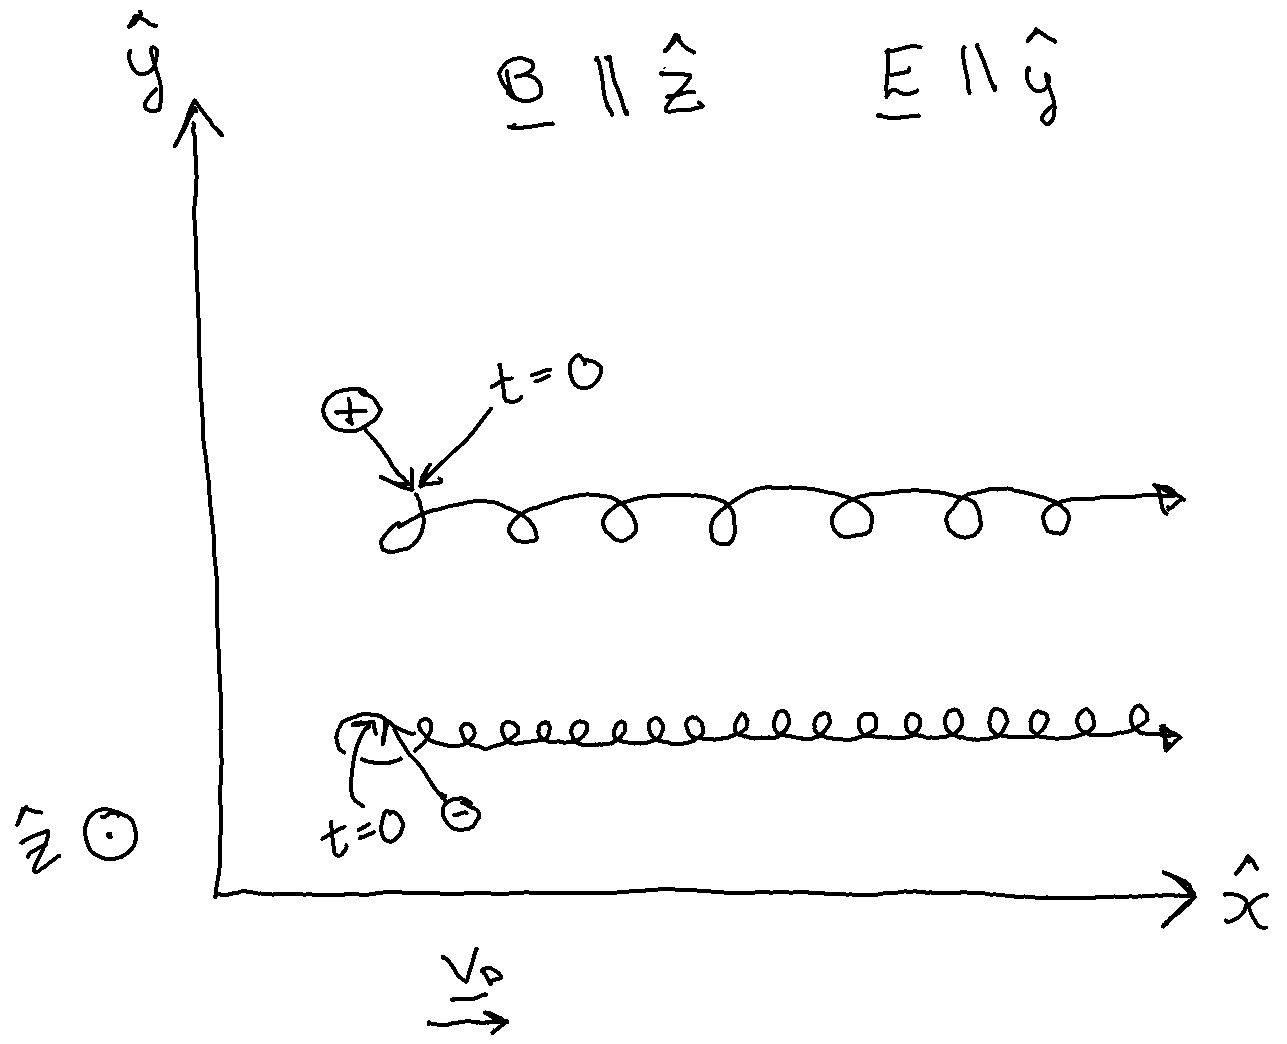
\includegraphics[width=.95\linewidth]{bilder/L7_ExB.png}
            \caption{}\label{fig:L7_ExB}
        \end{subfigure}
        \begin{subfigure}[t]{.3\linewidth}
            \centering
            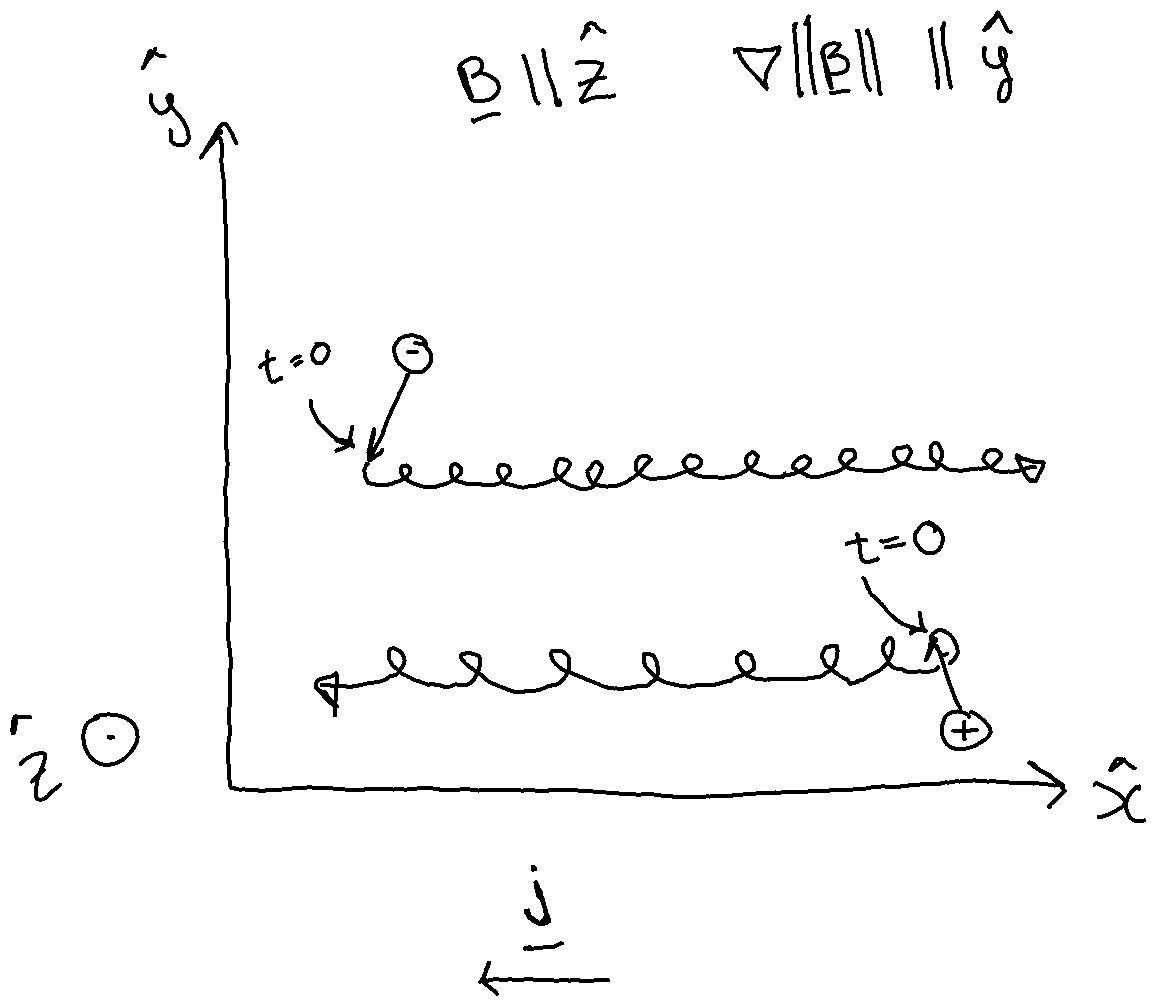
\includegraphics[width=.95\linewidth]{bilder/L7_gradB.png}
            \caption{}\label{fig:L7_gradB}
        \end{subfigure}
        \begin{subfigure}[t]{.3\linewidth}
            \centering
            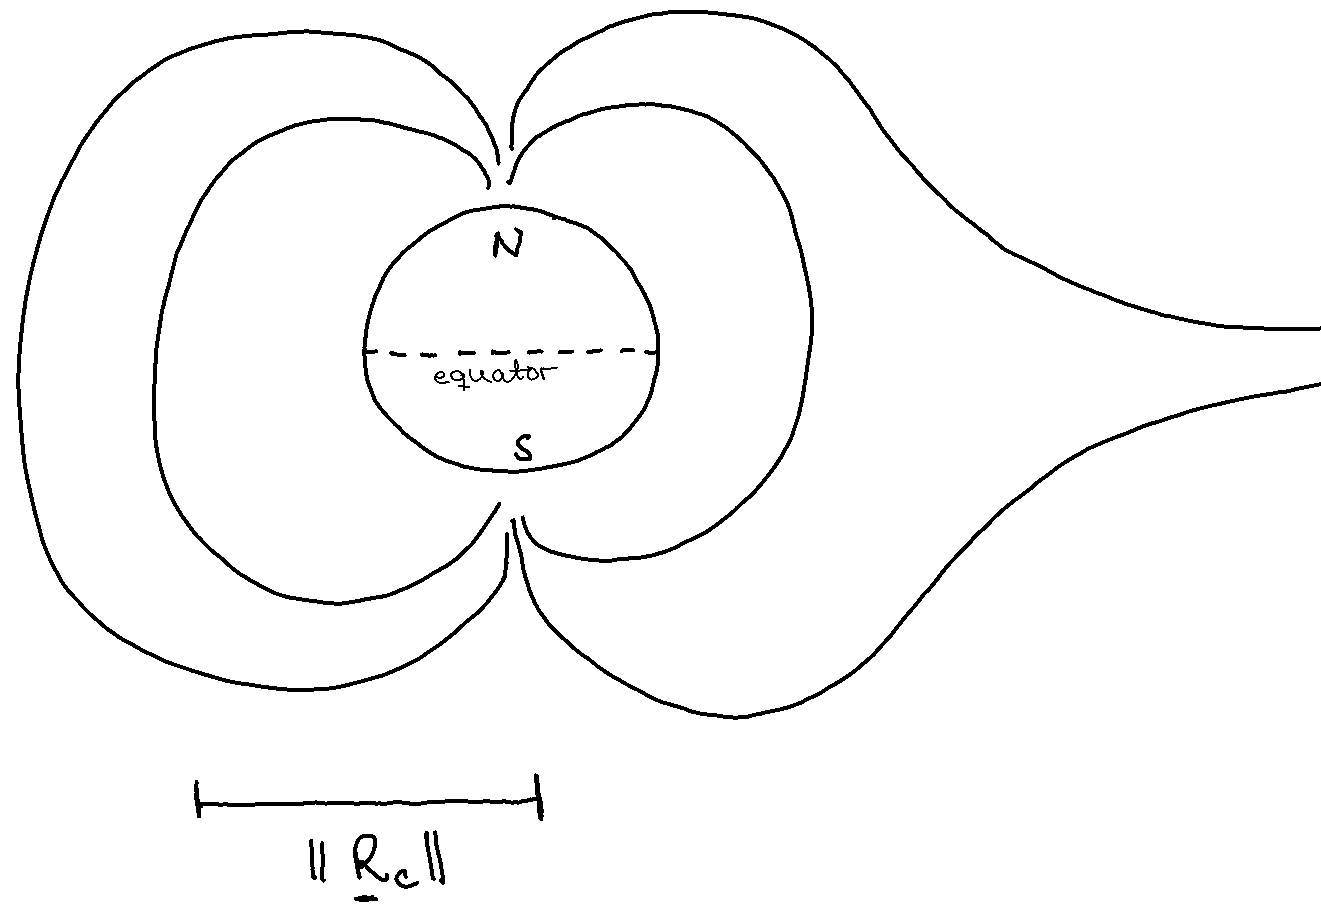
\includegraphics[width=.95\linewidth]{bilder/L7_curvB.png}
            \caption{}\label{fig:L7_curvB}
        \end{subfigure}

        \caption{Three nice drawings.}\label{fig:L7_ex1}
    \end{figure}
    \item [\textbf{EXERCISE 2 --- Prob. 5 Exam 1996}] The set of linearized equations for a cold plasma approximation is given by
    \begin{align*}
        \p{t}{\rho_1}+\nabla\cdot\left(\rho_0 \gf{v}_1\right)&=0\\
        \rho_0\p{t}{\gf{v}_1}&=-\frac{1}{\mu_0}\gf{B}_0\times\left(\nabla\times\gf{B}_1\right)\\
        \p{t}{\gf{B}_1}&=\nabla\times\left(\gf{v}_1\times\gf{B}_0\right)
    \end{align*}
    \begin{enumerate}[(a)]
        \item What is the essential assumption for the ``cold'' plasma approximation?
        \mylinbrk{}
        The essential assumption for a cold plasma approximation is that it is cold enough for pressure to be neglected. Pressure differences can't propagate.
        \item Let us introduce a small perturbation in the plasma, \(\gf{u}=\gf{u}_1\), \(\rho=\rho_0+\rho_1\), \(\gf{B}=\gf{B_0}+\gf{B_1}\). Linearize the set of MHD-equations under the assumption that the background magnetic field and the plasma density are constant.
        \mylinbrk{}
        The linearization is done already.
        \item We want to derive the dispersion relation for a cold plasma given the equations above. We assume normal mode solutions and rewrite the differential operators to get
        \begin{align*}
            -i\omega\rho_1+i\rho_0\gf{k}\cdot\gf{\widetilde{v}}_1&=0\\
            -i\omega\rho_0\gf{\widetilde{v}}_1&=-\frac{1}{\mu_0}\gf{\widetilde{B}}_0\times\left(i\gf{k}\times\gf{\widetilde{B}}_1\right)\\
            -i\omega\gf{\widetilde{B}}_1&=i\gf{k}\times\left(\gf{\widetilde{v}}_1\times\gf{\widetilde{B}}_0\right)
        \end{align*}
        By using the well known vector identity, the triple vector product \(\gf{A}\times\left(\gf{B}\times\gf{C}\right)=\left(\gf{A}\cdot\gf{C}\right)\gf{B}-\left(\gf{A}\cdot\gf{B}\right)\gf{C}\), and by letting \(\gf{k}=k\f{x}\) we can write this as
        \begin{align}
            -\omega\rho_1+\rho_0kv_{1x}&=0\label{eq:L7_alfven_normalmode1}\\
            -\omega\rho_0\gf{\widetilde{v}}_1&=-\frac{1}{\mu_0}\left[\left(\gf{\widetilde{B}}_0\cdot\gf{\widetilde{B}}_1\right)k\f{x}-B_{0x}k\gf{\widetilde{B}}_1\right]\label{eq:L7_alfven_normalmode2}\\
            -\omega\gf{\widetilde{B}}_1&=kB_{0x}\gf{v}_1-kv_{1x}\gf{\widetilde{B}}_0\label{eq:L7_alfven_normalmode3}
        \end{align}
        We choose our coordinate system such that \(\gf{\widetilde{B}}_0=\left[B_0\cos\theta,0,B_0\sin\theta\right]\), which yields
        \begin{align*}
            -\omega\rho_1+\rho_0kv_{1x}&=0\\
            -\omega\rho_0\gf{\widetilde{v}}_1&=-\frac{1}{\mu_0}\left[\left(B_{1x}B_0\cos\theta+B_{1z}B_0\sin\theta\right)k\f{x}-B_{0}\cos\theta k\gf{\widetilde{B}}_1\right]\\
            \gf{\widetilde{B}}_1&=\frac{-1}{\omega}kB_{0}\cos\theta\gf{v}_1+\frac{1}{\omega}kv_{1x}\gf{\widetilde{B}}_0
        \end{align*}
        where we can decompose \(\gf{\widetilde{B}}_1\) into
        \begin{equation*}
            \left(\begin{array}{c}
                B_{1x}\\
                B_{1y}\\
                B_{1z}
            \end{array}\right)=\frac{1}{\omega}\left(\begin{array}{c}
                B_0kv_{1x}\cos\theta-B_0kv_{1x}\cos\theta \\
                0-B_0kv_{1y}\cos\theta \\
                B_0kv_{1x}\sin\theta-B_0kv_{1z}\cos\theta
            \end{array}
            \right)
        \end{equation*}
        where we notice that \(B_{1x}=0\). Plugging this into our second equation yields
        \begin{equation*}
            \frac{\omega^2}{k^2}\gf{\widetilde{v}}_1=\frac{1}{\rho_0\mu_0}\left[\left(B_0v_{1x}\sin\theta-B_0v_{1z}\cos\theta\right)B_0\sin\theta\f{x}-B_{0}\cos\theta\left(
                \begin{array}{c}
                    0\\
                    -B_0v_{1y}\cos\theta \\
                    B_0v_{1x}\sin\theta-B_0v_{1z}\cos\theta
                \end{array}
                \right)\right]
        \end{equation*}
        The left hand side have all components of \(\gf{\widetilde{v}}_1\) in one term, while the right hand side have terms that include one of the components only in a given term. We move everything over to the left hand side and write the equation on matrix form with respect to the velocity vector. By doing this we obtain
        \begin{equation}\label{eq:L7_alfven_matrix_form}
            \left(
                \begin{array}{ccc}
                    \frac{\omega^2}{k^2}-\frac{B_0^2}{\rho_0\mu_0}\sin^2\theta &0&\frac{B_0^2}{\rho_0\mu_0}\cos\theta\sin\theta \\
                    0&\frac{\omega^2}{k^2}-\frac{B_0^2}{\rho_0\mu_0}\cos^2\theta &0\\
                    \frac{B_0^2}{\rho_0\mu_0}\cos\theta\sin\theta &0&\frac{\omega^2}{k^2}-\frac{B_0^2}{\rho_0\mu_0}\cos^2\theta
                \end{array}
            \right)\left(\begin{array}{c}
                    v_{1x}\\
                    v_{1y}\\
                    v_{1z}
                \end{array}
            \right)=\gf{0}
        \end{equation}
        where
        \begin{equation*}
            v_A^2=\frac{B_0^2}{\rho_0\mu_0},\quad\tn{Alfvén speed}
        \end{equation*}
        The dispersion relation can now very simply be found by assuming no trivial solutions exist. This means that the determinant of the matrix must be zero, hence
        \begin{equation*}
        \begin{aligned}
            \det\left(
                \begin{array}{ccc}
                    \frac{\omega^2}{k^2}-\frac{B_0^2}{\rho_0\mu_0}\sin^2\theta &0&\frac{B_0^2}{\rho_0\mu_0}\cos\theta\sin\theta \\
                    0&\frac{\omega^2}{k^2}-\frac{B_0^2}{\rho_0\mu_0}\cos^2\theta &0\\
                    \frac{B_0^2}{\rho_0\mu_0}\cos\theta\sin\theta &0&\frac{\omega^2}{k^2}-\frac{B_0^2}{\rho_0\mu_0}\cos^2\theta
                \end{array}
            \right)=0\\
            \left(\frac{\omega^2}{k^2}-v_A^2\cos^2\theta\right)\left(\frac{\omega^2}{k^2}-v_A^2\right)=0
        \end{aligned}
        \end{equation*}
        We see that this has two solutions, which will manifest themselves as two different Alfvén modes, namely
        \begin{align}
            \frac{\omega^2}{k^2}=v_A^2\cos^2\theta\quad&\sim\quad\tn{shear Alfvén wave mode}\label{eq:L7_shear_alfven_mode}\\
            \frac{\omega^2}{k^2}=v_A^2\quad&\sim\quad\tn{compressional wave mode}\label{eq:L7_compression_mode}
        \end{align}
        In the figure from \citet{1995Itsp}, they use a Poynting flux vector, defined as \(\gf{S}=\frac{1}{\mu_0}\gf{E}_1\times\gf{B}_1\), showing the direction of the propagation of the wave energy. We can investigate this further, plugging \cref{eq:L7_shear_alfven_mode} into the top row of \cref{eq:L7_alfven_matrix_form}. This gives
        \begin{equation*}
            \left(v_A^2\cos^2\theta-v_A^2\sin^2\theta\right) v_{1x}+v_A^2\cos\theta\sin\theta v_{1z}=0
        \end{equation*}
        Doing the same with the bottom row will lead to the implication that \(v_{1x}=v_{1z}=0\) while \(v_{1y}\) can take any value. But from \cref{eq:L7_alfven_normalmode1} we see that \(v_{1x}=0 \Rightarrow \rho_1=0\). It also affect \cref{eq:L7_alfven_normalmode3}, in which \(v_{1x}=0 \Rightarrow \gf{B}_1\vert\vert\gf{v}_1\perp\gf{B}_0\). We can then look at the size of the components \(\gf{B}_0\) and \(\gf{B}_1\)
        \begin{equation*}
            \left\vert\gf{B}_0+\gf{B}_1\right\vert=B_0^2+\underbrace{2\gf{B}_0\cdot\gf{B}_1}_{=0}+\cancelto{0}{B_1^2}
        \end{equation*}
        \(\therefore \) Magnetic pressure is constant.
        \item In the case of warm plasma the dispersion relation is given by:
        \begin{equation*}
            \left(\omega^2-k^2v_A^2\cos^2\theta\right)\left[\omega^4-\omega^2k^2\left(c_s^2+v_A^2\right)+k^4v_A^2c_s^2\cos^2\theta\right]=0
        \end{equation*}
        Identify the possible solutions/wave modes and discuss the Friedrich's diagram for the phase velocity, as shown in the top left diagram in \cref{fig:L7_alfven_waves}, i.e.\ the case where \(v_A=2c_s\).
        \mylinbrk{}
        What we see is that the two modes are recognized as
        \begin{align*}
            \frac{\omega^2}{k^2}&=v_A^2\cos^2\theta \\
            \frac{\omega^2}{k^2}&=\frac{1}{2}\left \{c_s^2+v_A^2\pm \sqrt{{\left(c_s^2+v_A^2\right)}^2-4c_s^2v_A^2\cos^2\theta}\right \}
        \end{align*}
        where the first dispersion relation give the intermediate mode and the second give the fast and slow modes. Looking closer at the second dispersion relation, we notice that if
        \begin{align*}
            \theta=0:\quad\frac{\omega^2}{k^2}&=\frac{1}{2}\left \{c_s^2+v_A^2\pm\left(c_s^2-v_A^2\right)\right \} \\
            \theta=\frac{\pi}{2}:\quad\frac{\omega^2}{k^2}&=\frac{1}{2}\left \{c_s^2+v_A^2\pm\left(c_s^2+v_A^2\right)\right \}
        \end{align*}
        \begin{minipage}{.4\linewidth}
            \begin{align*}
                \theta&=0 \rightarrow \gf{k}||\gf{B}\\
                \frac{\omega^2}{k^2}&=v_A^2\\
                \frac{\omega^2}{k^2}&=c_s^2
            \end{align*}
        \end{minipage}
        \begin{minipage}{.4\linewidth}
            \begin{align*}
                \theta&=\frac{\pi}{2} \rightarrow \gf{k}\perp\gf{B}\\
                \frac{\omega^2}{k^2}&=c_s^2+v_A^2~\tn{(FAST)}\\
                \frac{\omega^2}{k^2}&=0~\tn{(SLOW)}
            \end{align*}
        \end{minipage}
        \item Waves generated at the magnetopause can be observed behind Earth's bow shock. Only one of the MHD wave modes modes can travel from the magnetopause to the nose of the bow shock. Which wave mode is it? Qualify our answer.
        \mylinbrk{}
        My guess is that, since moving from the magnetopause to the bow shock means moving through the IMF, which then means the wave moves with a component perpendicular to the IMF, only the fast mode will be able to propagate over.
    \end{enumerate}
\end{enumerate}
\begin{figure}[t]
    \centering
    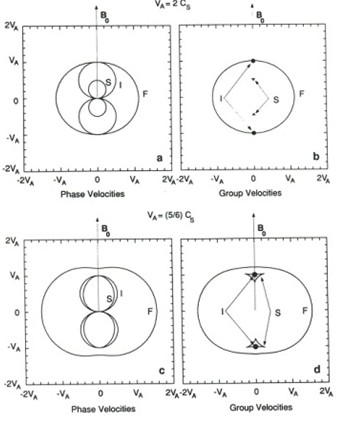
\includegraphics[width=.6\linewidth]{bilder/L7_alfven_waves.jpg}
    \caption{The fast (F), slow (S) and Alfvén wave (I) for \(v_A=2v_S\) (top) and \(v_A=5/6v_S\) (bottom).}\label{fig:L7_alfven_waves}
\end{figure}

\section[Standing waves]{Standing waves (K\&R 11.6)}
Let \(\ell=\) distance between the two ionospheres/hemispheres. A standing wave will then have
\begin{equation*}
    \lambda_{||}=\frac{2\ell}{n}
\end{equation*}
where \(n\in\mathbb{N}\) which is for a shear Alfvén wave. We also have
\begin{equation*}
    \frac{\omega}{k}=v_A\cos\theta\Rightarrow\frac{\omega}{k\cos\theta}=v_A=\frac{\omega}{k_{||}}
\end{equation*}
Further, we write \(k\) in terms of \(\lambda \) to gain information about the frequency.
\begin{equation*}
    f=\frac{\omega}{2\pi}=\frac{n\pi}{2\ell}v_A=\frac{n}{2\ell}\frac{B}{\sqrt{\mu_0\rho}}
\end{equation*}


\chapter{Magnetic reconnection}
\begin{remark}
    Section made from lectures done by Mike Kosch. Other sources are \citet{1995Itsp} --- chapter 9 \& parts of chapter 13.
\end{remark}

\section{Solar wind}
The hot solar corona (plus solar flares and coronal mass ejections) overcomes gravity and results in a wind, i.e.\ hot plasma (95\% protons and electrons) radiating outwards from the Sun to fill the interplanetary vacuum. We gain information about the magnetic field by looking at the polarization of light.

\subsection{Collisionless plasma?}
We take a look back at \cref{eq:magnitude_magnetic_field} to make sure we remember it. Due to the frozen in condition, the magnetic field strength of the sun at L1 is much higher than the geometry would suggest. The mean free path, i.e.\ the average distance between collisions is
\begin{equation*}
    \ell=\frac{k_{B}T}{\sqrt{2}\pi d^2p}
\end{equation*}
where \(p\) is pressure and \(d\) is the distance between protons.\\
\begin{minipage}[t]{.5\linewidth}
    \textbf{Is the solar wind collisionless?}\\
    Proton: \(d=\num{1.65e-15}\) m\\
    Pressure: \(p=\num{1e-4}-\num{1e-15}\) Pa\\
    Fast solar wind: \(T_i\approx 1500\) K, \(\ell >\num{1.7e13}\) m\\
    Slow solar wind: \(T_i\approx \num{8e5}\) K, \(\ell >\num{9e15}\) m
\end{minipage}
\begin{minipage}[t]{.5\linewidth}
    \textbf{Is the ionosphere (\SI{250}{\kilo\metre}) collisionless?}\\
    Proton: \(d=\num{1.65e-15}\) m\\
    Pressure: \(p=\sim\num{1e-4}\) Pa\\
    Oxygen amount \(=16\) \\
    \(T_i\approx 1500\) K, \(\ell >\num{1.1e12}\) m\\
    \(1 AU \approx\num{1.5e11}\) m
\end{minipage}

\subsection{Frozen in magnetic flux}
When investigating the frozen in magnetic flux, we will need Ohm's law, \(\gf{j}=\sigma\left(\gf{E}+\gf{u}\times\gf{B}\right)\), the condition of collisionless plasma giving \(\sigma=\infty \) and therefore \(\gf{E}=-\gf{u}\times\gf{B}\), i.e.\ convection applies.
\begin{equation*}
    \gf{j}=\sigma\left(\gf{E}+\gf{u}\times\gf{B}\right)
\end{equation*}
and then the Lorentz' force give
\begin{equation*}
    \gf{F}=q\left(\gf{E}+\gf{u}\times\gf{B}\right)=q\gf{E}+\gf{I}\times\gf{B}
\end{equation*}
\begin{equation*}
    \frac{\gf{j}}{\sigma|_\infty}=0=\gf{E}+\gf{u}\times\gf{B}
\end{equation*}
From this we get that if we have no electric field we also have no velocities, or if we do have velocities, we will also have an electric field. How is this possible? The answer is blowing in the wind, or rather, magnetic field lines is stuck in the solar wind.

\subsection{What controls the solar wind?}
Typical solar wind forces at 1 AU are a plasma pressure of \(p=nk_{B}T\) (\(\sim \num{1.3e-13}\)), a magnetic pressure of \(p=B^2/2\mu_0\) (\(\sim \num{1.4e-11}\)) and a dynamic pressure of \(p=\rho u^2\) (\(\sim \num{1.7e-9}\)). We see that at this point, the dynamic pressure is by far the dominating process.

\section{SuperDARN radars}
Coherent scatter radars with Tx peak power \(=\SI{9.6}{\kilo\watt}\) at \(8\)--\(\SI{20}{\mega\hertz}\). The range is \(\sim 1000\)--\(\SI{3000}{\kilo\metre}\) with a range resolution of \(15\)--\(\SI{45}{\kilo\metre}\). The time resolution is \(\sim\SI{120}{\second}\) and you have 16 beams. 12 radars is located in the southern hemisphere, while in the northern hemisphere there are 22 radars.

Their main objective is to observe plasma flow in the ionosphere at \(200\)--\(\SI{300}{\kilo\metre}\) altitude. The radars can only see backscatter with right angles to the field lines. Field aligned plasma irregularities like stritiations and scintillations have frequencies of
\begin{equation*}
    \Delta f=\frac{\Delta v}{c}f_0
\end{equation*}

Coherent backscatter is what the technique is called, or alternatively Bragg scattering. Bragg's law for crystals (coherent scatter) is given as
\begin{equation}\label{eq:L8_bragg_scatter}
    n\lambda=2d\sin\theta
\end{equation}
From the SuperDARN radars, we get data to add to the convection flow maps.

\section{Thin current sheets}
Discontinuities of magnetic electric field result in currents. From Ampere's law we have
\begin{equation*}
    \oint_C\gf{B}\cdot\tn{d}\gf{\ell}=\mu_0\iint_S\gf{j}\cdot\tn{d}\gf{S}=\mu_0I_{enc}
\end{equation*}
Regions of distinctly different magnetic field are separated by current sheets, e.g.\ the magnetopause of magnetotail neutral sheet. Ampere's law applies, hence the current sheets. Current sheets are ``thin'', e.g.\ \SI{100}{\kilo\metre} (versus \(10\)--\(100 R_E\)).

\subsection{Magnetopause/magnetotail position}
The location of the magnetopause is where the solar wind dynamic pressure balances the magnetosphere magnetic pressure.
We find the distance to the ring current and assume \(B_z<0\) to get the balancing equation
\begin{equation*}
    nmu^2=\frac{{(2\cdot 13)}^2}{2\mu_0}=\frac{4{\left(\frac{B_0}{r^3}\right)}^2}{2\mu_0}
\end{equation*}
where \(B_0=\num{31000}\si{\nano\tesla}\), \(\mu_0=4\pi 10^{-7}\), \(u\) is the solar wind speed, \(n\) the solar wind density and \(m=m_p\). We end up with an expression for the distance \(r\) given as
\begin{equation*}
    r=\sqrt[6]{\frac{2B_0^2}{nmu^2\mu_0}}=9.85 R_E
\end{equation*}

Looking at the magnetopause in closer detail, we first make the assumption that \(\gf{B}=\gf{0}\). When the particles meet the magnetic field of the Earth, they start gyrating, ions down and electrons up. This gives a current moving down, and we look at the magnitude by checking how many, first ions, that crosses any given horizontal line (flux) (\cref{fig:L8_magnetopause_flux}). We know that flux is given as
\begin{equation*}
    \xi=2rnu
\end{equation*}
and for current we have
\begin{equation*}
    I=2r nuq=\xi q
\end{equation*}
For a loop going through our region of interest we get
\begin{equation*}
    \mu_0 I=B_z+0+0+0 \Rightarrow I=\frac{B_z}{\mu_0}
\end{equation*}
\begin{equation*}
    \frac{B_z}{\mu_0}=2r nuq\Rightarrow r=\frac{mu}{qB_z}
\end{equation*}
\begin{equation*}
    \underset{\substack{\uparrow \\ \tn{magnetic}\\ \tn{pressure}}}{\frac{B_z^2}{2\mu_0}}=\underset{\substack{\uparrow \\ \tn{dynamic}\\ \tn{pressure}}}{mu^2}
\end{equation*}
We may also take a look at how thick the magnetopause is.
\begin{equation*}
    r=\frac{mu}{qB},\quad B=\frac{B_0}{r^3}\approx \SI{31}{\nano\tesla}
\end{equation*}
\begin{equation*}
    \Rightarrow r=\SI{16.8}{\kilo\metre}
\end{equation*}
where we have used \(u=\SI{500}{\kilo\metre/\second}\), \(m=m_p\) and \(q\) is the elementary charge.
\begin{figure}[t]
    \centering
    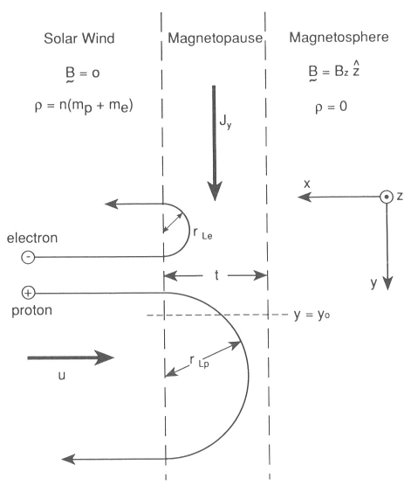
\includegraphics[width=.4\linewidth]{bilder/L8_magnetopause_flux.jpeg}
    \caption{Flux of ions and electrons crossing through a line in the \(xy\)-plane in the magnetopause.}\label{fig:L8_magnetopause_flux}
\end{figure}

\section{The geomagnetic tail}
Here we find reservoirs of plasma and energy, and this is associated with substorms. The magnetic field strength in the near/far Earth tail lobe is generally \(B=20/\SI{10}{\nano\tesla}\) respectively.

\subsection{Plasma beta (\(\beta \))}
Plasma beta is defined as
\begin{align*}
    \tn{plasma beta}&=\frac{\tn{plasma thermal pressure}}{\tn{magnetic pressure}}\\
    \beta&=\frac{nk_{B}T}{B^2/2\mu_0}
\end{align*}
We can find the width of the magnetotail by looking at the total magnetic flux close to the Earth (polar cap) and compare this to the total magnetic flux in the tail. This yields
\begin{align*}
    \phi=\int \gf{B}\cdot\tn{d}\gf{S},\quad \phi_{pc}=\phi_T\\
    \Rightarrow \phi=BA
\end{align*}
For the polar cap, this can fairly easily be found
\begin{equation*}
    \phi_{pc}=2B_0\left[\pi{\left(R_E\sin\theta_{pc}\right)}^2\right]
\end{equation*}
where \(\theta_{pc}\sim \SI{15}{\degree}\) and the term \(2B_0\) appears because of the dipole approximation, \(B_0\) at the equator and \(2B_0\) at the pole. With a value of \(B_T=\SI{20}{\nano\tesla}\) or \(B_T=\SI{10}{\nano\tesla}\) this gives us (found from \(B_T^2/2\mu_0=nk_B(T_e-T_i)\))
\begin{equation*}
    r_T=20 R_E\quad\tn{and}\quad r_T=29 R_E
\end{equation*}

\subsection{Tail flaring}
Tail flaring is an effect we see due to the interaction of solar wind vs.\ magnetic pressure. This give an unstable situation similar to what you would see from a flag blowing in strong wind.

The total mass of the magnetosphere can be found to be, using the numbers that gave us \(r_T=29R_E\) and a length of \(1000R_E\) and a number density \(n=\num{0.3e6}\) we have
\begin{equation*}
    \tn{mass}=1000R_E\pi{\left(29R_E\right)}^2nm_p\approx \num{3.42e5}\si{\kilo\gram}=342\tn{ tons}
\end{equation*}
Here, we have used \(nmu^2\sin\theta=B^2/2\mu_0\) due to the widening of the magnetotail.

\section{Magnetic reconnection \& the Dungey cycle}
\subsection{\(B_z\) negative}
For the solar wind, the Reynolds number get very high. The conductivity is practically infinite, scale lengths are large and velocities are huge. The Reynolds number is defined as
\begin{equation*}
    Re=\frac{VL}{\eta},\quad\eta=\frac{1}{\mu_0\sigma_0}
\end{equation*}
For magnetic reconnection we need the frozen-in conditions to break down, i.e.~\(Re\leq 1\), which give diffusion. We look at the induction equation
\begin{equation*}
    \p{t}{\gf{B}}=\nabla\times\left(\gf{u}\times\gf{B}\right)+\frac{\nabla^2\gf{B}}{\mu_0\sigma_0}
\end{equation*}
We assume \(u\approx 0\), hence
\begin{equation*}
    \p{t}{\gf{B}}=\frac{\nabla^2\gf{B}}{\mu_0\sigma_0}
\end{equation*}
Let \(\gf{B}||\mathbf{x}\) so that \(\p{y}{B_x}=0=\p{x}{B_x}\).
\begin{equation*}
    \p{t}{B_x}=\frac{1}{\mu_0\sigma_0}\p{zz}{B_x}=0
\end{equation*}
We get the diffusion equation and we see that the \(x\)-component of \(B\) is constant along the \(z\)-direction. The steady state assumption gives us
\begin{equation*}
    \p{t}{B_x}=0\Rightarrow\p{z}{B_x}=\tn{constant}
\end{equation*}
We now impose an electrical field, included in Ohm's law from the frozen-in condition
\begin{equation*}
    E_y=-u_{z}B_x
\end{equation*}
Faraday's law tells us that
\begin{equation*}
    \nabla\times\gf{E}=\p{t}{\gf{B}}=0
\end{equation*}
From this we see that since \(B_x\) is constant through time then \(E_y\) is constant. Therefore \(u_z\) must be constant. In the diffusive zone we have \(E_y=j_y/\sigma_0\), and here we make use of Ampere's law to look at the current
\begin{align*}
    \oint\gf{B}\cdot\tn{d}\gf{\ell}&=\mu_0 I\\
    B_{x}x+0+\left(-B_x\right)\left(x\right)+0&=\mu_0 I\\
    2B_{x}x&=\mu_0 I
\end{align*}
\begin{equation*}
    \therefore j_y=\frac{I}{x2\ell}=\frac{B_x}{\ell\mu_0}
\end{equation*}
Now, notice that the electric field should be constant in our region, both in the diffusive zone and the convective zone. Combining the expressions for the two cases where \(E_y\) appears gives us
\begin{equation*}
    E_y=\frac{B_x}{\ell\mu_0\sigma_0}=-u_{z}B_x
\end{equation*}
\begin{equation}\label{eq:L8_ell_relation_reynold}
    u_z\mu_0\sigma_0\ell=1
\end{equation}
which is the Reynolds number. What this means is that the frozen-in condition does not apply in this scenario, and we allow for plasma to move across magnetic filed lines.

But where does the energy go? It will be transferred to the electrons, and we get a hint by looking at Fick's law of diffusion
\begin{equation*}
    J=-\mu_0k_{B}T\p{x}{n}
\end{equation*}
where \(J\) is the flux and \(n\) is the number density. The size of the electrical field that the solar wind carries can be found from looking at the velocity of the solar wind and the strength of the magnetic field:
\begin{equation*}
    E=-u_{sw}B_{sw}=\SI{400}{\kilo\metre/\second}\times\SI{6}{\nano\tesla}=\SI{2.4}{\milli\volt/\metre}
\end{equation*}
The polar cap potential can be found from this. We again use that the polar cap reaches \(\theta=\SI{15}{\degree}\) from the pole, giving a radius of \(r_{pc}=\theta R_E=\SI{1500}{\kilo\metre}\). Thus
\begin{equation*}
    \Phi_{pc}=E2r_{pc}=\SI{8}{\kilo\volt}
\end{equation*}

We can find the distance downstream at where the reconnection takes place. Again we use \(u_{sw}=\SI{400}{\kilo\metre/\second}\) and the time it takes the field lines to convect over the polar cap is simply \(t=2r_{pc}/v_{pc}=2\times\SI{1500}{\kilo\metre}/\SI{330}{\metre/\second}\approx 10^4\si{\second}\).
\begin{equation*}
    D_x=u_{sw}t\approx 600R_E
\end{equation*}
We might assume a polar cap potential of \(\Phi_{pc}=\SI{60}{\kilo\volt}\). If we use a width of the tail of \(D=50R_E\) with \(B_{sw}=\SI{5}{\nano\tesla}\) we end up with a potential across the tail of
\begin{equation*}
    \Phi=ED=B_{sw}u_{sw}D=\SI{640}{\kilo\volt}
\end{equation*}
What we notice is that this potential might be ten times the potential at the polar cap, meaning most particles do not get trapped and hence do not precipitate down to the Earth.
\begin{figure}[t]
    \centering
    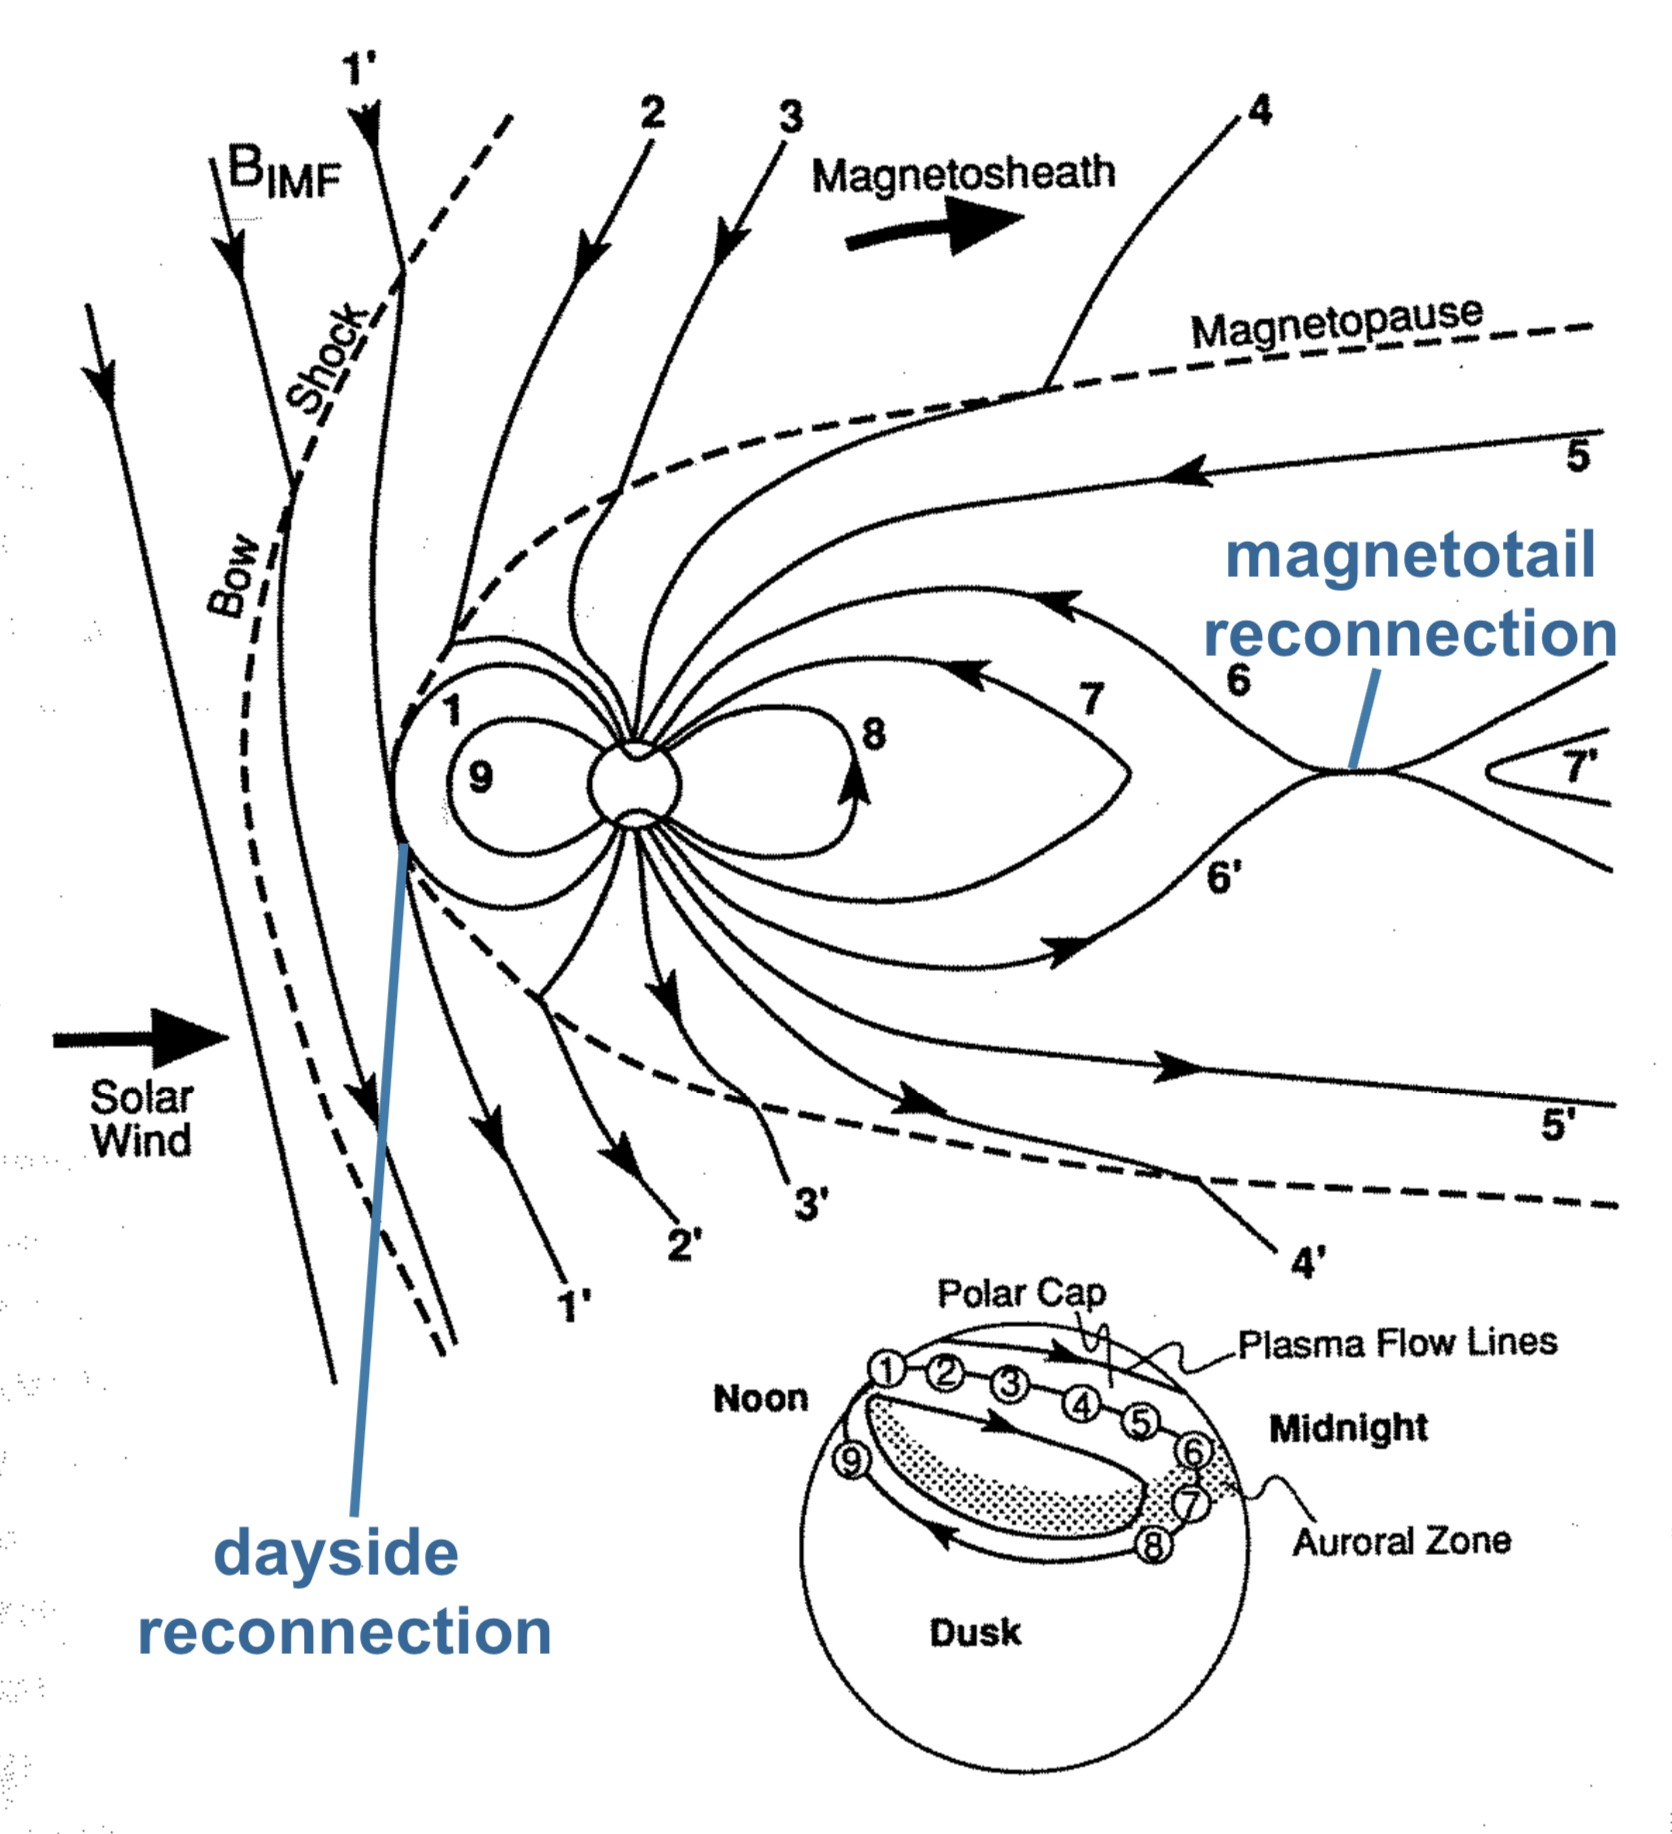
\includegraphics[width=.4\linewidth]{bilder/L8_dungey_cycle.jpg}
    \caption{The Dungey cycle.}\label{fig:L8_dungey_cycle}
\end{figure}

\subsection{Reconnection asymmetry}
For \(B_y<0\) or \(B_y>0\) we get different convection patterns. The reconnection asymmetry we get for \(B_y<0\) (points towards dusk) is a banana that lies on the dusk side, and vice versa. We also see a shift of the dayside OCB in the direction of the \(B_y\) component.
\begin{figure}[t]
    \centering
    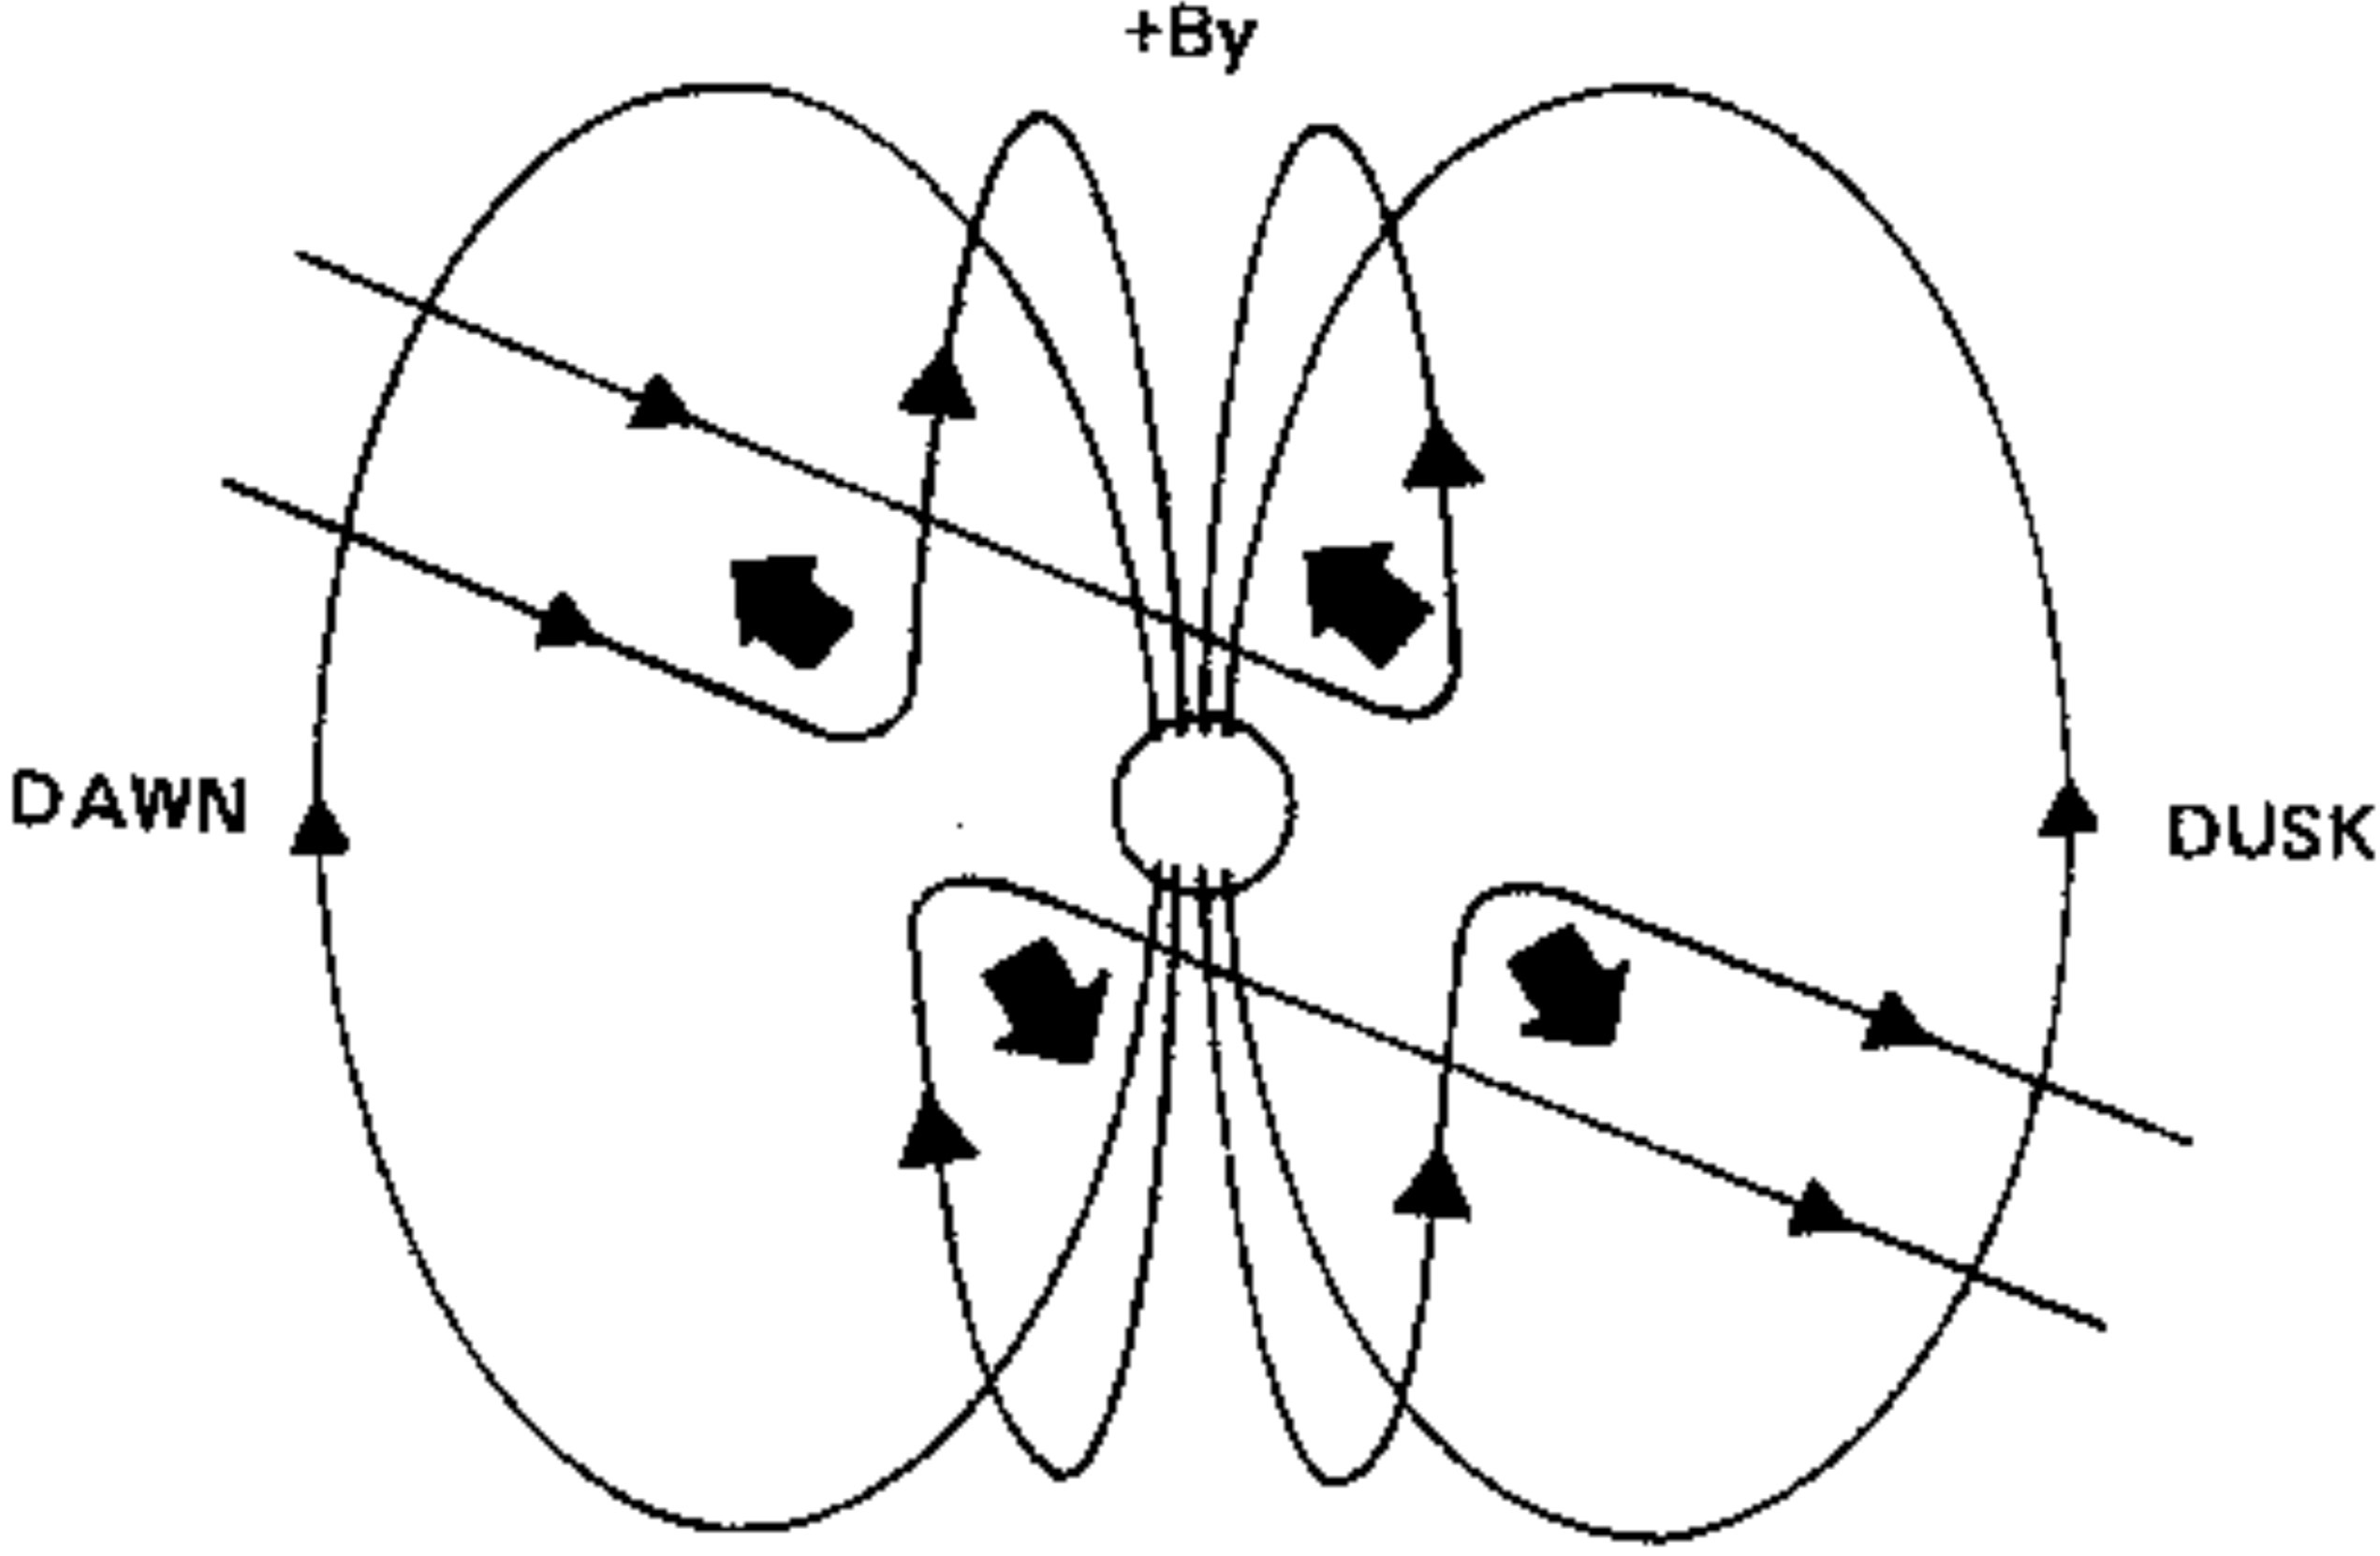
\includegraphics[width=.4\linewidth]{bilder/L8_by_asymmetry.jpg}
    \caption{\(B_y\) positive seen from the sun.}\label{fig:L8_by_asymmetry}
\end{figure}

\subsection{\(B_z\) positive}
For positive IMF we also get reconnection, but at a much lower efficiency. It reconnects with the magnetic field of the Earth at bit behind the poles where closed lines have downward components. As usual, we also see reconnection on the nightside where the magnetic lines from the Earth meets up.

\subsection{Fluid description of reconnection}
Here, we will develop the MHD fluid descriptions of magnetic reconnection. The model will be time-stationary and two-dimensional. We start with the Sweet-Parker solution shown in \cref{fig:L8_mag_recon}. This is a basic \(x\)-line configuration. The shaded diffusion region is \(2L\) long and \(2\ell \) wide, where \(L\gg\ell \). We assume for simplicity that the inflow and outflow parameters are symmetrical. A reasonable assumption in the tail, not so much for the magnetopause. The electric field is spatially uniform and points out of the page, so that
\begin{equation*}
    E=u_{i}B_i=u_{o}B_o
\end{equation*}
We also assume that the flow is incompressible, i.e.\ that \(\rho_i=\rho_o=\rho \), and from conservation of mass we get
\begin{equation}\label{eq:L8_ell_relation_L}
    u_{i}L=u_o\ell
\end{equation}
We now turn our attention to the energy. We look at how the kinetic energy gained by the outflowing plasma compare to the electromagnetic energy flowing into the diffusion regions. The electromagnetic-energy inflow rate per unit area is given by the Poynting flux
\begin{equation*}
    |\gf{S}|=|\gf{E}\times\gf{H}|=\frac{EB_i}{\mu_0},\quad\gf{H}=\frac{\gf{B}}{\mu_0}
\end{equation*}
\begin{equation*}
    |\gf{S}|=\frac{u_{i}B_i^2}{\mu_0}
\end{equation*}
The mechanical energy out is given by the gain in kinetic energy of the outflowing plasma. The rate of energy gain per unit area in the incident flow is
\begin{equation*}
    \Delta W=\frac{1}{2}\rho_f u_i\left(u_o^2-\cancelto{0}{u_i^2}~~~\right)
\end{equation*}
where \(\rho_f\) is the flow rate.
\begin{align*}
    \frac{u_{i}B_i^2}{\mu_0}&=\frac{1}{2}\rho u_{i}u_o^2\\
    u_o^2&=\frac{2B_i^2}{\mu_0\rho},\quad v_A=\frac{B}{\sqrt{\mu_0\rho}}\\
    u_o^2&=2v_A^2
\end{align*}
where \(\rho \) denotes mass density. We use the expression from \cref{eq:L8_ell_relation_L} in the above equation to obtain
\begin{equation*}
    \frac{u_i^2L^2}{\ell^2}=2v_A^2
\end{equation*}
\begin{equation*}
    u_i=\frac{\sqrt{2}v_A\ell}{L}
\end{equation*}
From \cref{eq:L8_ell_relation_reynold}, we have that the Reynolds number is given as \(Re=1=\mu_0\sigma\ell u_i\) in the diffusion region. We substitute for \(\ell \) and obtain
\begin{equation*}
    u_i^2=\frac{\sqrt{2}v_A}{\mu_0\sigma L}
\end{equation*}
or equivalently
\begin{equation*}
    u_i=v_A\sqrt{\frac{\sqrt{2}}{Re}}
\end{equation*}
where \(v_A\approx\SI{510}{\kilo\metre/\second}\) is the solar wind speed. What we end up with is that in all solar-system plasmas for which \(Re\) is very large, the incoming velocity is way too low compared to the velocity we know the solar wind to have. Using \(\nu=5/3, T_i=\num{12e5}\si{\kelvin},T_e=\num{1.4e5}\si{\kelvin}, m_i=m_p\) we get \(v_s=\SI{53}{\kilo\metre/\second}\).

This was solved by Petchek, with the geometry shown in \cref{fig:L8_reconnection_new_solution}, when he realized that most of the plasma does not need to flow through the diffusion region to get accelerated, but can be accelerated in the region where MHD is still valid, in the convection region. We must have shock waves to obtain the force required to get reconnection in the diffusion region, shock waves that are connected to the diffusion region and that remain fixed in space. This removes the bottleneck caused by requiring that all plasma should flow within a length \(\ell \) in the midplane. The diffusion region is still important in this solution since it is here the reconnection has to happen, but, the region can be vanishingly small. Its size will not even enter our calculations.
\begin{figure}[t]
    \centering
    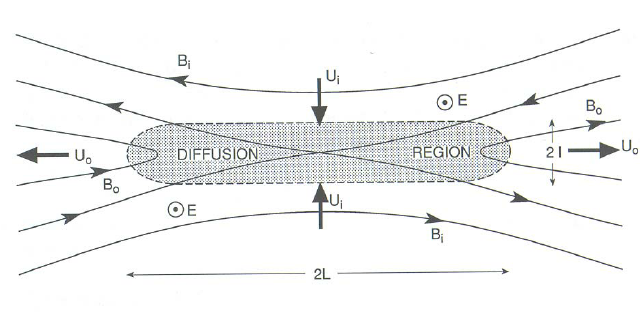
\includegraphics[width=.6\linewidth]{bilder/L8_mag_recon.png}
    \caption{The Sweet-Parker solution to magnetic reconnection.}\label{fig:L8_mag_recon}
\end{figure}
\begin{figure}[t]
    \centering
    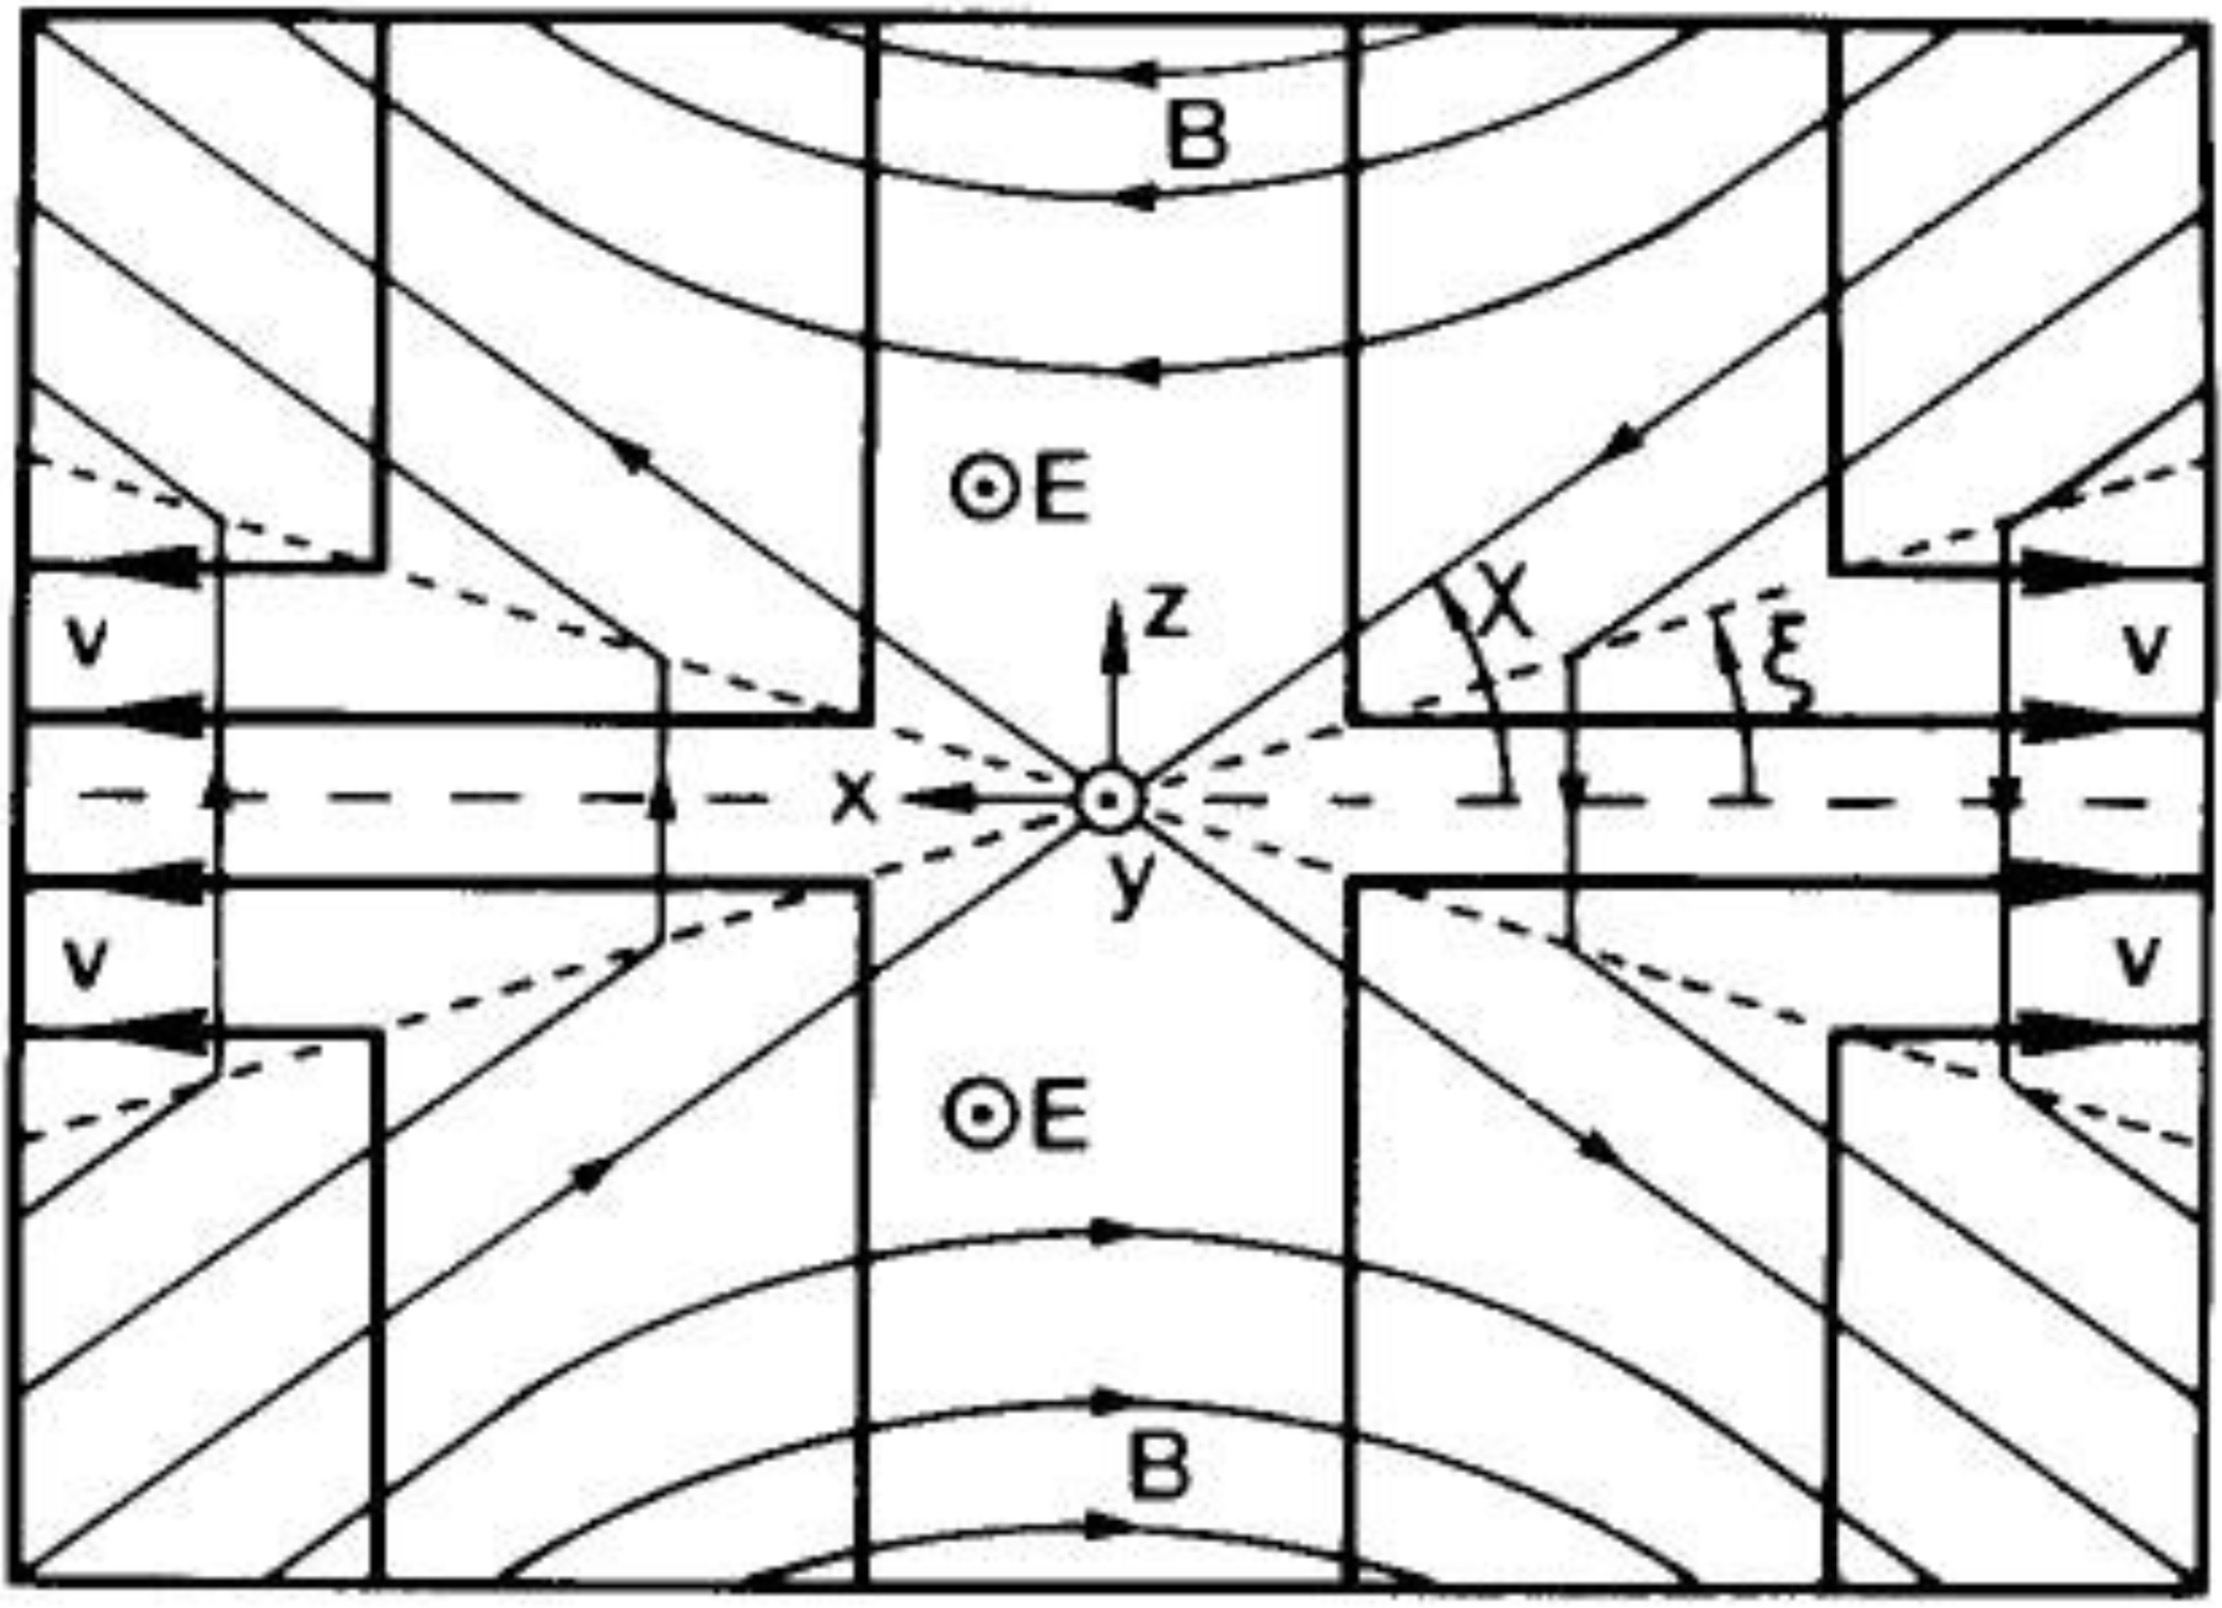
\includegraphics[width=.7\linewidth]{bilder/L8_reconnection_new_solution.jpg}
    \caption{The geometry of the new solution to reconnection proposed by Petchek.}\label{fig:L8_reconnection_new_solution}
\end{figure}

Shock waves form in gases and fluids in front of supersonic objects, or in front of objects within supersonic flows. Across the shock wave front, the properties of the gas (density, temperature, field strength, flow speed) change suddenly. If the kinetic energy is reduced, the thermal energy will be increased (\(k_{B}T\)). Generally, shocks are not adiabatic, i.e.\ not reversible. This implies energy dissipation, i.e.\ that entropy is increasing.

But how do shocks form in collision less plasma? Collisions are not required to form shocks. Electrostatic and electromagnetic forces can act. A shock must conserve mass, energy and momentum as well as obey the MHD equations.

Let \(Q\) be density and \(\gf{F}\) the flux. For conservation of mass, energy and momentum we get
\begin{equation*}
    \p{t}{Q}+\nabla\cdot\gf{F}=0
\end{equation*}
By assuming steady state and 1-dimension only we have
\begin{equation*}
    \p{x}{F_x}=0,\qquad\left(\gf{F}_{u}-\gf{F}_{d}\right)\cdot\f{x}=0,\qquad\left[F_x\right]=0
\end{equation*}
We then impose the MHD criteria of continuity
\begin{equation*}
    \p{x}{\rho u_x}=0,\qquad\left[\rho u_x\right]=0
\end{equation*}
From Maxwell's equations we have \(\nabla\cdot\gf{B}=0\), and by also enforcing that tangential \(\gf{E}_T\) must be preserved, i.e.~\(\nabla\times\gf{E}=-\p{t}{\gf{B}}\) we assume the steady state and frozen in condition \(\gf{E}=-\gf{u}\times\gf{B}\).

A termination shock is where gas of fluid goes from supersonic to subsonic without an intervening object, and it is similar to water in a sink. This may happen because the plasma is cooling
\begin{equation*}
    v_s=\sqrt{\frac{k_B\left(\gamma T_i+T_e\right)}{m_i}}
\end{equation*}
A termination shock forms where the solar wind meets the interstellar medium (\(T=10\)--\(\num{10000}\) K) at a distance of \(\sim 75\)--\(90\) AU\@.

\subsection{Bow shock}
\begin{enumerate}[\(\bullet \)]
    \item thickness: 100--1000\si{\kilo\metre}
    \item distance: \(13.5R_E\)
    \item solar wind mean free path \(>\) 1 AU
\end{enumerate}

\section{Open closed field lines}
\subsection[Viscous coupling]{Viscous coupling (K\&R p. 264)}
Another factor that let particles through to our magnetosphere is viscous coupling, although this is far less important compared to magnetic reconnection. It is a term used to include any process other than magnetic reconnection that can transport momentum across the magnetopause. It can include kinetic processes --- such as anomalous particle diffusion  via wave-particle interactions --- and large-scale fluid interactions. In the latter case, particles in the solar wind that drifts on the flanks of the magnetosphere can be caught by frictional forces due to a Kelvin-Helmholtz instability, or magnetopause distortions resulting from traveling pressure variations in the magnetosheath. A third concept --- impulsive plasma penetrations --- has also been proposed to contribute to this viscosity. These processes contribute to approximately 10--20\% of the particles that enter.

Flux transfer events are when we get an increase in particles that is moved into our magnetosphere.

\subsection[Ion upflow]{Ion upflow (K\&R p. 277)}
Imagine a magnetosheath consisting of \(\tn{H}^+\) that entered the magnetosphere and has just mirrored at low altitude on the field line labeled 2 in \cref{fig:L8_dungey_cycle}. The ion moves up the field line, and as it encounters weaker magnetic fields, its parallel velocity increases. Soon the pitch angle is close to zero, and if it is moving quickly it will soon reach the magnetopause again and reenter the magnetosheath. This may happen by the time the field line has convected to the position of of the field line labeled 3. A more slowly moving ion will exit the magnetosphere father down the tail, where lines 4 and 5 crosses the magnetopause. If the ion is sufficiently slow, it will still be on the magnetospheric portion of the filed line when the line reaches position 6, and what happens next depends on weather the ion is tailward or earthward of the \(x\)-line when the field line reconnects. If it is earthward, the ion will enter the current sheet on a closed field line and follow a Spieser-type orbit before it is accelerated towards the Earth.

We can quantitatively derive a relation among the speed at which the particle moves, the cross-tail potential drop, and the distance to the \(x\)-line to find what energy particles will enter the plasma sheet earthward of the neutral line. Let the distance to the ``pinch off''/\(x\)-line be \(L_x\) and assume the magnetic field lines to be straight. The time it takes an ion to reach the critical point will then be given as
\begin{equation*}
    t=\frac{L_x}{v_{||}}
\end{equation*}
We have the size of the electric field given as
\begin{equation*}
    E=\frac{\Phi}{2R_T}
\end{equation*}
and by combining this by use of the \(\gf{E}\times\gf{B}\) drift we get
\begin{equation*}
    t=\frac{2R_T^2B_T}{\Phi}
\end{equation*}
and
\begin{equation*}
    v_{||}=\frac{\Phi L_x}{2R_T^2B_T}
\end{equation*}
\begin{equation*}
    \therefore W_c=\frac{m}{2}{\left(\frac{\Phi L_x}{2R_T^2B_T}\right)}^2
\end{equation*}
where \(B_T\) is the lobe field strength and \(W_c\) is the critical particle energy. We may use \(L_x=100R_E, \Phi=\SI{53}{\kilo\volt},R_T=26R_E,B_T=\SI{10}{\nano\tesla}\).
\begin{equation*}
    \Rightarrow v_{||}=\SI{21}{\electronvolt}
\end{equation*}
Since we have \(T_i=T_e\approx\SI{1500}{\kelvin}=\SI{0.15}{\electronvolt}\) in the upper atmosphere, we see that there is a second order of magnitude less than what they need to gain to escape.

\subsection{Radiation belts}
The inner belt goes from \(0.01\)--\(1.5R_E\) with \(E_P\sim <\SI{100}{\mega\electronvolt}\) (protons) while the outer belt goes from \(3\)--\(10R_E\) with \(E_P\sim <\SI{10}{\mega\electronvolt}\) (electrons). The outer radiation belt is highly variable, but since the inner belt is on permanently closed magnetic field lines it is much more stable.

The particles accumulate because the loss is particularly weak here. Inner belt is caused by cosmic rays. They ionize what ever they come in contact with. The outer belt is mostly caused by reconnection, making it more unstable. In just a matter of hours, the outer radiation belt may die out and load up again.

\section{Auroral oval}
We expect to see symmetrical structures in the northern and southern hemispheres, but due to difficulties in knowing which filed lines maps to where between the hemispheres and the \(B_y\) skewing, among other things, this has been difficult to see.

Hall conductance gives the size of the magnetic field, but not the energy dissipation. The Birkeland currents are parallel to the magnetic field.

Region 1 currents (\cref{fig:L8_all_currents}) are more poleward than region 2 currents. Both can either be up or down, the region only tells you about latitude. The Harang\footnote{\href{https://nbl.snl.no/Leiv_Harang}{Leiv Harang}} discontinuity is where region 1 and 2 do not match up. Generally, auroras correspond to upward currents since this is where the downward electron flow is.

Hall current (electrojets) exists because it is a transition between collisionless and collisional plasmas.
\begin{figure}[t]
    \centering
    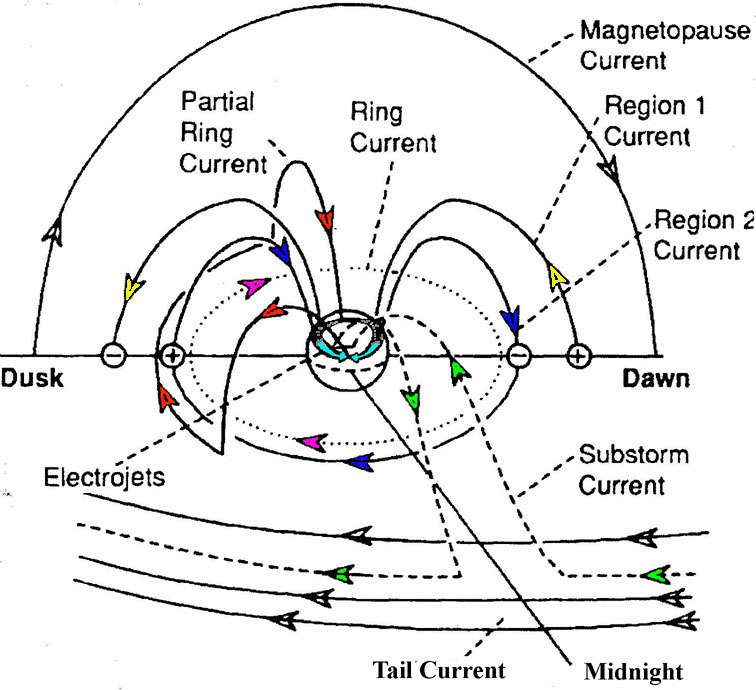
\includegraphics[width=.4\linewidth]{bilder/L8_all_currents.jpg}
    \caption{The currents we find in the magnetosphere. Depending on the precipitation and ionization the current may go straight past the Earth or down to the Earth and up.}\label{fig:L8_all_currents}
\end{figure}

\section{Substorms}
\subsection{Near Earth neutral line (NENL)}
The best developed model of substorms is the near-earth neutral-line (NENL) model. This model attempts to provide an internally consistent explanation for most magnetospheric phenomena, but does not attempt to explain many ionospheric observations. In the NENL model, a substorm begins when a southward turning of the IMF activates dayside reconnection. The start of the substorms come from particles precipitating from the NENL, illustrated in \cref{fig:L8_NENL_plasmoids}. The \(X\)-line is assumed to be inactive. Dayside magnetic flux from the Earth connects to the IMF and is transported over the polar caps by the solar wind, where it is added to the outer portions of the tail lobes. The removal of this flux from the dayside initiates a convective flow of plasma toward the reconnection region, but the flow is retarded by the finite conductivity of the ionosphere at the foot of the field lines. Because of this, the magnetospheric return flow is unable to balance the rate at which flux reconnects, and the dayside magnetopause erodes earthward.

Dayside erosion increases magnetopause flaring, thus increasing the dynamic pressure on the boundary, and this pressure reduces the flaring angle, compressing the tail until a corresponding increase in tail-lobe magnetic pressure balances the external pressure.

\subsection{Plasmoids (O-line)}
The unique feature of the NENL model is the formation of a \emph{plasmoid} that is ejected from the plasma sheet during the expansion and recovery phase of a substorm. The formation of a plasmoid is a direct consequence of the substorm growth phase that initiate the substorm. When the magnetic field lines bulge out again, these structures arise in the magnetotail behind the NENL\@.
\begin{figure}[t]
    \centering
    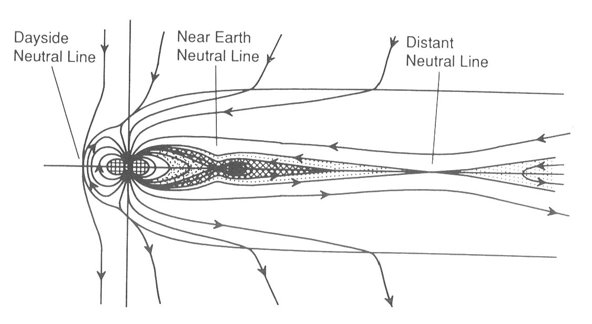
\includegraphics[width=.7\linewidth]{bilder/L8_NENL_plasmoids.jpeg}
    \caption{The location of the near Earth neutral line in the magnetotail and a plasmoid right behind it.}\label{fig:L8_NENL_plasmoids}
\end{figure}

\section{Important equations}
A summary of the most equations from this section is
\coloredeqq{
    \begin{aligned}
        p&=nk_{B}T&&\tn{---~~~Plasma pressure}\\
        p&=\frac{B^2}{2\mu_0}&&\tn{---~~~Magnetic pressure}\\
        p&=\rho{}u^2=nmu^2&&\tn{---~~~Dynamic pressure}\\
        \oint\gf{B}\cdot\tn{d}\gf{\ell}&=\mu_0I&&\tn{---~~~Ampere's law}\\
        \gf{F}&=q\left(\gf{E}+\gf{u}\times\gf{B}\right)&&\tn{---~~~Lorentz' law}\\
        \gf{j}&=\sigma\left(\gf{E}+\gf{u}\times\gf{B}\right)&&\tn{---~~~Ohm's law}\\
        \tn{Rm}&=\mu_0\sigma{}UL&&\tn{---~~~Magnetic Reynolds number}
    \end{aligned}
}


\chapter{The Sun \& the solar wind}
\begin{remark}
    Section made from lectures done by Kjellmar Oksavik. Other sources are \citet{BrekkeAsgeir2013Potu} --- chapter 1.
\end{remark}
\section{The solar atmosphere}
The temperature at the solar center is assumed to be as high as \(\num{1.5e7}\) K. At this high temperature protons will be converted to helium nuclei by thermonuclear reactions such as the proton–proton and carbon-cycle chains. The proton-proton chain can be illustrated as
\begin{align*}
    \pres{1}{}{H}+\pres{1}{}{H}&\rightarrow \pres{2}{}{H}+e^++\nu+\SI{0.42}{\mega\electronvolt}\\
    \pres{1}{}{H}+\pres{2}{}{H}&\rightarrow \pres{3}{}{He}+\gamma+\SI{5.5}{\mega\electronvolt}\\
    \pres{3}{}{He}+\pres{3}{}{He}&\rightarrow \pres{4}{}{He}+2\pres{1}{}{H}+\SI{12.8}{\mega\electronvolt}
\end{align*}
where \(e^+\), \(\nu \) and \(\gamma \) represent a positron, a neutrino and a gamma ray quantum, respectively.

When we look at the Sun's atmosphere, we divide it into three parts. \Cref{fig:L9_zones_in_the_sun} show a schematic of the zones of the Sun, namely the core, the radiation zone and the convection zone. The innermost region reaching out to about 600 km above the top of the convection zone is the \emph{photosphere}. It typically consists of negative hydrogen ions. The photosphere absorb the visible radiation from below because there are so many negative electrons. The temperature is decreasing with height as shown in \cref{fig:L9_sun_temperatures}. Between 600 and \(\num{2000}\) km is the \emph{chromosphere}. This region is transparent in the visible spectrum (except some absorption lines). The temperature is increasing with height. Between the chromosphere and the corona we find the transition region, where the temperature is dramatically increasing to the order of \(10^5\) K. Outside of the chromosphere is the \emph{corona}. This region is fully ionized, and electrons cannot stick to the atoms anymore. It is structured, isothermal and dependant on the magnetic field. Temperatures are of \(\orderof{(6)}\).
\begin{figure}[t]
    \centering
    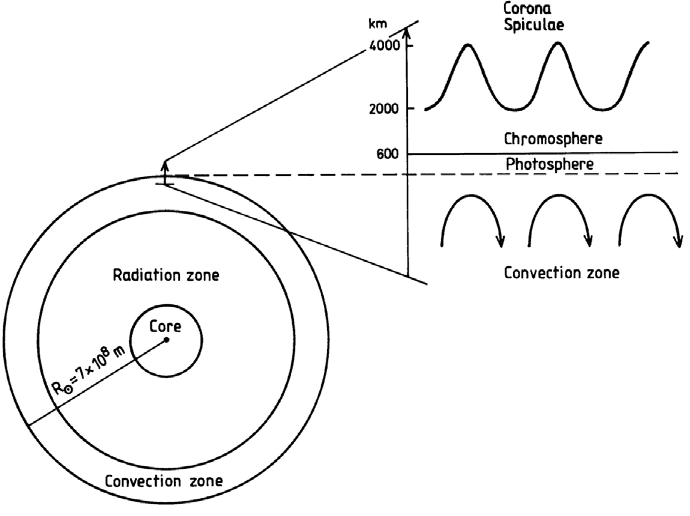
\includegraphics[width=.6\linewidth]{bilder/L9_zones_in_the_sun.png}
    \caption{A schematic diagram showing the different zones of the Sun; the core, the radiation zone and the convection zone.}\label{fig:L9_zones_in_the_sun}
\end{figure}
\begin{figure}[t]
    \centering
    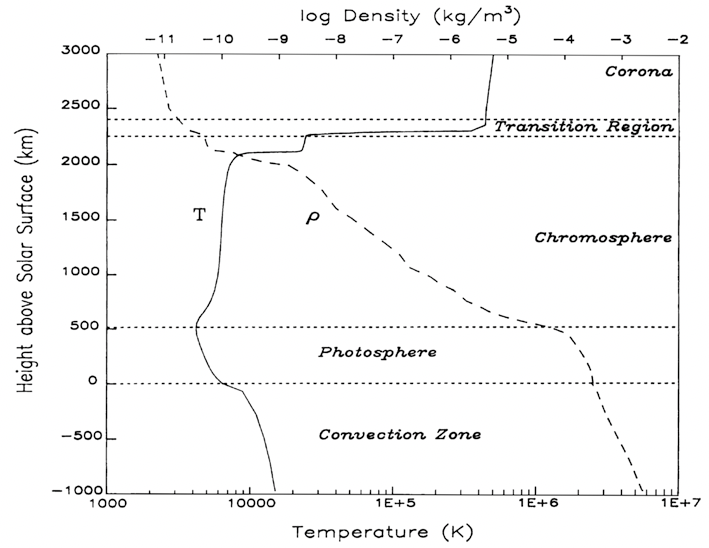
\includegraphics[width=.6\linewidth]{bilder/L9_sun_temperature.png}
    \caption{Temperature and density profiles in the solar atmosphere showing the steep temperature increase in the transition region. The zero level refers to about one solar radius from te center of the solar disk.}\label{fig:L9_sun_temperatures}
\end{figure}

\section{Electromagnetic radiation from the Sun}
The observed radiation spectrum from the Sun as measured from the Earth's surface in the wavelength region \(200\)--\(\SI{3200}{\nano\metre}\) is shown in \cref{fig:L9_sun_spectral_irradiance}. The solar spectrum, as observed outside the Earth's atmosphere, compared to that of a blackbody, give a temperature of \SI{6000}{\kelvin}.

Ultraviolet (UV) and X-ray radiation shorter than 200 nm are strongly absorbed by air. The UV radiation region is usually divided into two parts. (1) the far ultraviolet (FUV) region between 100 and 200 nm coming from the upper photosphere. It is absorbed in the mesosphere/thermosphere. (2) the extreme ultraviolet (EUV) region between 10 and 100 nm coming from the chromosphere. There are some strong emission lines from this, such as the hydrogen Balmer lines at \SI{121.6}{\nano\metre} (\(Ly_\alpha \)), \SI{102.5}{\nano\metre} (\(Ly_\beta \)), etc., the helium line at 58.4 nm and the oxygen line at 130.4 nm.

For spectral irradiance and the variability, we have the largest variabilities for \(\lambda <\SI{300}{\nano\metre}\).
\begin{figure}[t]
    \centering
    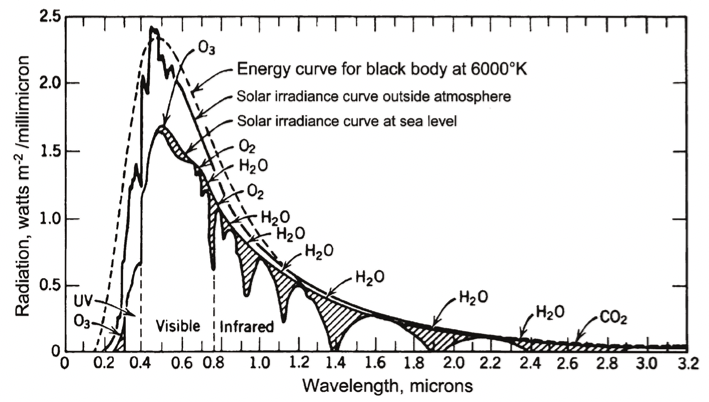
\includegraphics[width=.6\linewidth]{bilder/L9_sun_spectral_irradiance.png}
    \caption{The Sun's spectral irradiance per unit wavelength of solar radiation observed at sea level compared with a blackbody spectrum at \(\num{6000}\) K and the spectrum observed outside the Earth's atmosphere.}\label{fig:L9_sun_spectral_irradiance}
\end{figure}

\section{Planck's radiation law}
Let us assume that the Sun is radiating its energy approximately as a blackbody with temperature \(T\), then the spectral brightness, \(B_\nu \), per frequency band, \(\tn{d}\nu \), according to Planck's radiation law will be
\begin{equation*}
    B_\nu=\frac{2h\nu^3}{c^2}\frac{1}{\exp\left(\frac{h\nu}{kT}\right)-1},\qquad \left[\si{\watt\hertz^{-1}}\tn{sr}^{-1}\si{\metre^{-1}}\right]
\end{equation*}
where \(B_\nu \) is given in the frequency range \(\nu \) to \(\nu+\tn{d}\nu \). We notice that it only depends on the temperature and not the geometry of the body. We can also express the spectral brightness \(B_\lambda \) per unit wavelength band between \(\lambda \) and \(\lambda+\tn{d}\lambda \) in the following manner when noting that \(\tn{d}\nu=-\left(c/\lambda^2\right)\tn{d}\lambda \) and \(B_\nu\tn{d}\nu=B_\lambda\tn{d}\lambda \):
\begin{equation*}
    B_\lambda=\frac{2hc^2}{\lambda^5}\frac{1}{\exp\left(\frac{hc}{k\lambda T}\right)-1}
\end{equation*}
We find that the maximum in \(B_\lambda \) (\(\p{\lambda}{B_\lambda}=0\)) occurs at the wavelength \(\lambda_m\) which satisfies
\begin{equation*}
    5\left(1-e^{-x_m}\right)=x_m
\end{equation*}
where
\begin{equation*}
    x_m=\frac{hc}{k\lambda_m T}
\end{equation*}
The solution can be found numerically to be \(x_m=4.9651\dots \), which then finally gives
\begin{equation*}
    \lambda_{m}T=\num{2.898e-3}\si{\metre\kelvin}
\end{equation*}
which is the \emph{Wien displacement law} expressing that the wavelength at maximum radiation for a blackbody is inversely proportional to the temperature. \Cref{fig:L9_blackbody_radiation} demonstrates the Wien displacement law where \(B_\lambda \) is presented for different temperatures. We had a maximum in the solar spectrum close to \SI{500.0}{\nano\metre} which then gives a temperature of
\begin{equation*}
    T=\SI{5780}{\kelvin}
\end{equation*}

According to the Stefan-Boltzmann law, which is the integrated Planck's equation over all wavelengths and solid angles, we have the total radiated power \(Q\) given by
\begin{equation}\label{eq:L9_stefan_boltzmann}
    Q=qS=\sigma T^4S
\end{equation}
where \(S\) is the surface of the radiating body and \(q\) is the radiated power per unit area. The Stefan-Boltzmann constant \(\sigma \) is given by
\begin{equation*}
    \sigma=\frac{2\pi^5k^4}{15c^2h^3}=\num{5.67e-8}\si{\watt\metre^{-2}\kelvin^{-4}}
\end{equation*}
For the Sun, the radiated power per unit area is
\begin{equation*}
    q_\odot=\sigma T_\odot^4=\num{6.3e7}\si{\watt\metre^{-2}}
\end{equation*}
The total radiated power from the Sun will be
\begin{equation*}
    Q_\odot=4\pi R_\odot^2q_\odot=\num{3.9e26}\si{\watt}
\end{equation*}
The power that is reaching Earth we can find by assuming that the power flux is conserved.
\begin{equation*}
    E_e=q_\odot{\left(\frac{R_\odot}{r}\right)}^2=\SI{1380}{\watt\metre^{-2}}
\end{equation*}
\begin{figure}[t]
    \centering
    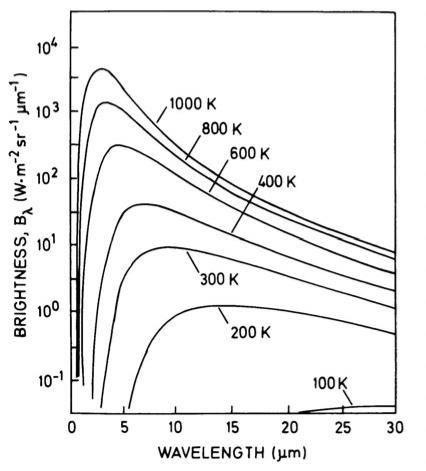
\includegraphics[width=.4\linewidth]{bilder/L9_blackbody_radiation.png}
    \caption{Curves showing blackbody radiation functions for bodies with different temperatures.}\label{fig:L9_blackbody_radiation}
\end{figure}

\section{The greenhouse effect}
The heat radiated from the Sun is the main heat source for the Earth and its atmosphere, but to maintain an equilibrium temperature we need a comparable loss of heat radiation. The blackbody radiation from the Earth is
\begin{equation*}
    Q_e=4\pi R_e^2\sigma T_e^4
\end{equation*}
while the absorption of the radiation from the Sun is
\begin{equation*}
    Q_{se}=\left(1-\alpha\right)E_e\pi R_e^2
\end{equation*}
where \(\alpha \) is the albedo or reflection coefficient (\(\approx 0.3\)). For thermal equilibrium we need \(Q_{se}=Q_e\), but this gives
\begin{equation*}
    T_e={\left(\frac{(1-\alpha)E_e}{4\sigma}\right)}^{1/4}=\SI{255}{\kelvin}
\end{equation*}
I.e.\ we need a green house effect to explain the discrepancy. The average temperature on the surface is \(T_e=288\) K, which according to the Wien displacement law give infrared radiation.

Let us now assume that the atmosphere has a temperature \(T_a\), and that it radiate accordingly. The heat balance we now get is
\begin{equation*}
    \sigma 4\pi R_e^2T_e^4=2\sigma 4\pi R_e^2T_a^4
\end{equation*}
and by solving for \(T_a\) we find
\begin{equation*}
    T_a^4=\frac{1}{2}T_e^4
\end{equation*}

We now include the heat from the sun, and the balance become \(Q_{se}+\frac{1}{2}Q_a=Q_e\), and by insertion we can solve for \(T_e\) and obtain
\begin{equation*}
    T_e={\left[\frac{(1-\alpha)E_e}{2\sigma}\right]}^{1/4}=\SI{304}{\kelvin}
\end{equation*}

\section{Radio wave emissions from the Sun}
For radio frequencies corresponding to the wavelength regime we have \(10^4\)--\(10^2\si{\mega\hertz}\). The energy related to this is typically \(h\nu=\num{6.6e-25}\si{\joule}\). This is much less than the thermal energy for a reasonable solar temperature which corresponds to \(kT_\odot=\num{8.4e-20}\si{\joule}\). Because of this, we can use the Rayleigh-Jeans approximation of Planck's radiation law (\(k\nu\ll kT\))
\begin{equation}\label{eq:L9_rayleigh_jeans}
    B_\nu=\frac{2h\nu^3}{c^2}\frac{1}{1+h\frac{\nu}{kT}+\cdots -1}=\frac{2kT\nu^2}{c^2}
\end{equation}
\Cref{fig:L9_solar_radiowave_radiation_spectrum} show a schematic diagram of the solar radio wave radiation spectrum for a quiet Sun as well as for the slowly varying component (the S-component). (From Tohmatsu, 1990.)

We now look at \cref{fig:L9_sun_earth_geometry}. We notice that the radiation energy emitted from an infinitesimal area \(\tn{d}\sigma \) perpendicular to the Sun-Earth line at a point \(P\) on the Sun and hitting the surface of the Earth is
\begin{equation*}
    \tn{d}I_\nu=B_\nu\tn{d}\sigma\Omega=B_\nu\tn{d}\sigma\frac{S}{r_1^2}
\end{equation*}
where \(S\) is the projection of the surface of the Earth facing the Sun on a plane perpendicular to the line from \(P\) to the Earth's center, \(r_1\) is the distance from \(P\) to the Earth \(r_1\gg R_e\) and \(\Omega=S/r_1^2\) is the solid angle corresponding to the surface \(S\) seen from \(P\). We assume the brightness to be isotropic, and that \(r\gg R_\odot \) so that \(r=r_1\). The total radiation flux per unit area reaching the Earth is then
\begin{equation*}
    \phi_\nu=\frac{I_\nu}{S}=\int_\Sigma B_\nu\frac{\tn{d}\sigma}{r^2}=\pi{\left(\frac{R_\odot}{r}\right)}^2B_\nu
\end{equation*}
where \(\Sigma \) is the Sun's effective area. Substituting in from \cref{eq:L9_rayleigh_jeans} gives
\begin{equation*}
    \phi_\nu=\pi{\left(\frac{R_\odot}{r}\right)}^2\frac{2k}{c^2}\nu^2T=\pi{\left(\frac{R_\odot}{r}\right)}^2\frac{2kT}{\lambda^2}
\end{equation*}
We plug in the proper constants and end up with
\begin{equation}\label{eq:L9_rad_flux}
    \phi_\nu=\num{2.09e-44}\nu^2T\quad \left[\si{\watt\metre^{-2}\hertz^{-1}}\right]
\end{equation}

For the 10.7 cm radio flux we find from \cref{eq:L9_rad_flux} that the radiation flux is given by (\(F_\lambda=\phi_\nu/\nu^2\))
\begin{equation*}
    F_{10.7}=\num{16.4e-26}T
\end{equation*}
and the index is therefore a direct indicator of the effective temperature. The 10.7 is also directly correlated with electron density, hence its importance.

We introduce the electron plasma frequency given by
\begin{equation*}
    f_{pe}=\frac{1}{2\pi}{\left(\frac{n_{e}e^2}{m_{e}\varepsilon_0}\right)}^{1/2}=K\sqrt{n_e}
\end{equation*}
From a given level of the solar atmosphere characterized by a specific electron density of \(n_e\) only radiation with a frequency \(\nu >f_{pe}\) will escape if the influence of the magnetic field is neglected. \Cref{fig:L9_variations_in_electron_density} show that electron density decreases strongly from close to \(10^{15} \si{\metre^{-3}}\) at \(1R_\odot \) to close to \(10^{10} \si{\metre^{-3}}\) at \(10R_\odot \). According to our understanding of the plasma frequency we now realize that by observing radio emissions from the Sun at increasing frequencies (or decreasing wavelengths) we are probing deeper and deeper into the solar atmosphere. It is found that while m-waves are formed far out in the corona, cm-waves are generated deep in the solar atmosphere and mm-waves penetrate almost all the way from the photosphere. 99\% of the energy: \(\lambda=276\)--\(\SI{4960}{\nano\metre}\), 99.9\% of the energy: \(\lambda=217\)--\(\SI{10940}{\nano\metre}\). Only 0.1\% is outside of the visible, IR and UV\@.
\begin{figure}[t]
    \centering
    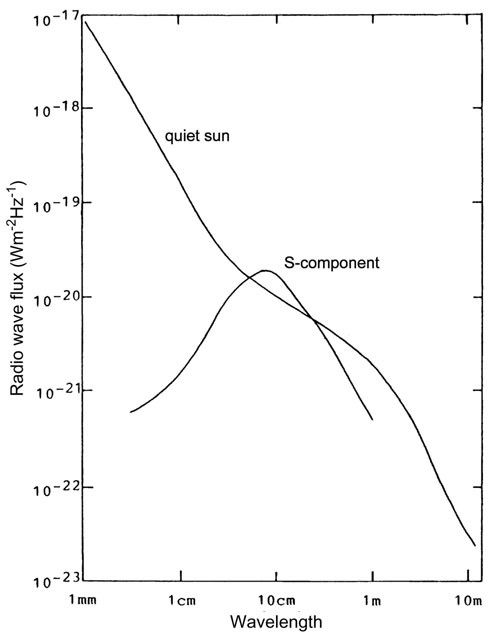
\includegraphics[width=.4\linewidth]{bilder/L9_solar_radiowave_radiation_spectrum.jpg}
    \caption{Schematic diagram of the solar radiowave radiation spectrum for a quiet Sun as well as for the slowly varying component (the \(S\)-component).}\label{fig:L9_solar_radiowave_radiation_spectrum}
\end{figure}
\begin{figure}[t]
    \centering
    \includegraphics[width=.9\linewidth]{bilder/L9_sun_earth_geometry.png}
    \caption{The Sun–Earth geometry where \(S\) is the projection of the Earth's surface to a plane perpendicular to the Sun-Earth line, \(r\) is equal to 1 AU, and \(\tn{d}\sigma \) is the projection of an infinitesimal area on to a plane perpendicular to the line from a point \(P\) on the Sun to the Earth's center. Since \(r\gg R_\odot \), where \(R_\odot \) is the solar radius, \(r_1\) can be considered equal to \(r\).}\label{fig:L9_sun_earth_geometry}
\end{figure}
\begin{figure}[t]
    \centering
    \includegraphics[width=.4\linewidth]{bilder/L9_variations_in_electron_density.jpg}
    \caption{Variations in electron density in the solar atmosphere from the base of the photosphere to a distance of 10 \(R_\odot \) from the center of the solar disk under different solar activity conditions.}\label{fig:L9_variations_in_electron_density}
\end{figure}

\section{Sunspots \& the solar cycle}
A sunspot was first observed by Galileo. The solar cycles have a period of on average eleven years.

The fact that sunspots come and go in cycles was not appreciated until 1843. After some time, Wolf devised a quantitative definition for a sunspot number and studied sunspot data for the years 1700 to 1848. In its present form the Wolf sunspot number \(R_z\) is defined as
\begin{equation}\label{eq:L9_wolf_sunspot_number}
    R_z=k\left(10g+f\right)
\end{equation}
where \(f\) is the total number of sunspots regardless of size, \(g\) is the number of sunspot groups and \(k\) is a normalization constant accounting for the different observatories.

\section{Electromagnetic radiation from a disturbed Sun}
The most short-lived phenomenon observed from Earth on the solar surface is the flare event which usually occurs within a region encompassed by a large magnetically complex bipolar sunspot group.

Let us assume by inspecting \cref{fig:L9_variations_in_electron_density} that the electron density at a distance \(z\) from the solar surface is
\begin{equation*}
    n_e(z)=n_{e0}\exp\left(-\frac{z-z_0}{H}\right)
\end{equation*}
where \(n_{e0}\) is the electron density at a reference height \(z_0\) and \(H\) is the \(e\)-folding scale height. From the expression of plasma frequency we find
\begin{equation*}
    \fracd{f_{pe}}=K\frac{1}{2}n_e{(z)}^{-1/2}\fracd[z]{n_e(z)}\fracd{z}=-\frac{f_{pe}}{2H}\fracd{z}
\end{equation*}
and the propagation velocity \(v_{RS}\) of the radio source emitting a radio frequency \(f\) equal to the instantaneous plasma frequency \(f_{pe}\) is given by
\begin{equation*}
    v_{RS}=\fracd{z}=-2H\fracd{}\ln f
\end{equation*}
During the first minutes of development after the flare flash has occurred, groups of very narrow bursts appear that show a fast drift from high to low frequency.
\begin{enumerate}
    \item [\emph{Type III}] Right after the flare, narrow, fast relativistic electrons in the corona, \(v=0.2\)--\(0.9c\). Originate at \(50\)--\(100 R_\odot \)
    \item [\emph{Type V}] 1--3 min after Type III
    \item [\emph{Type II}] Slower, last 5--10 min, appears 5 min after Type III, \(v=500\)--\(1500\si{\kilo\metre/\second}\), EM shock waves
    \item [\emph{Type IV}] A broad continuum, 10 min to hours. Trapped relativistic particles
    \item [\emph{Type I}] Hours to days. Not related to flares. Might be caused by large sunspots
\end{enumerate}

\section{Particle emissions from the Sun}
A quiet Sun radiates not only electromagnetic waves, but also particles. A solar wind is always blowing. This wind is not a steady wind, but rather gusty as it varies quite strongly in velocity as well as density at a distance from the Sun corresponding to the Earth’s orbit.

Under quiet conditions the wind has a medium velocity of \SI{400}{\kilo\metre/\second} but can, however, vary between 200 and \SI{700}{\kilo\metre/\second} (takes 1--5 days to the Earth). The density is often between \(10^6\) and \(\num{2e7}\si{\metre^{-3}}\). The average energy of the protons is of the order of 1 keV while the electrons have energies of the order of 1 eV. The average particle flux from the Sun can be estimated to be
\begin{equation*}
    \phi=nv\approx\num{2e12}\si{\metre^{-2}\second^{-1}}
\end{equation*}
Total average particle loss per unit time form the Sun is therefore
\begin{equation*}
    \p{t}{N}=4\pi R_\odot^2\phi\approx\num{1.23e31}\si{\second^{-1}}
\end{equation*}
By neglecting the mass of the electrons in the solar wind, this particle loss per unit time corresponds to a mass loss per unit time given by
\begin{equation*}
    \p{t}{m}=\p{t}{N}m_p=\num{2.21e5}\si{\kilo\gram/\second}
\end{equation*}
which is a loss much smaller than what we have from radiation (\(\num{4.3e9}\si{\kilo\gram/\second}\)). The proton temperature in the solar wind is \(10^4\)--\(\num{2e5}\si{\kelvin}\) while the electron temperature is a factor of 3--4 larger. The magnetic field strength varies between 1 and \SI{15}{\nano\tesla}, where on average we have \(T_{||}\approx 2T_\perp \).

Of the characteristic parameters we have given for the solar wind so far, we notice that the speed of sound of the solar wind gas is approximately
\begin{equation*}
    C_s=\sqrt{\frac{\gamma kT_\odot}{m_p}}=\num{1.17e4}\si{\metre/\second}
\end{equation*}
where \(\gamma=5/3\) is the adiabatic constant and \(T_\odot=10^4\) K. Since the solar wind is on average 30 times higher, the solar wind is supersonic. The place where the solar wind turns subsonic due to pressure forces from the interstellar medium is called the heliopause.

\section{Fluid flow in a nozzle}
Let an incompressible gas with density \(\rho \) stream through a tube with a varying cross-section \(A\). Since mass flux through any cross-section of the tube must be constant, we have
\begin{equation*}
    \phi_m=A\rho v=\tn{const}
\end{equation*}

The pressure gradient will be balanced by the inertia force when no other forces are acting in the equation of motion. Considering only one dimension along \(r\) we have
\begin{equation*}
    \fracd{p}=-\rho\fracd{v}=-\rho\fracd[r]{v}v
\end{equation*}
Using \(\tn{d}p=-\rho v\tn{d}v\), we can plug this into our expression. Thus
\begin{align}
    \frac{\tn{d}p}{\rho}=\fracd[\rho]{p}\frac{\tn{d}\rho}{\rho}=-v\tn{d}v\notag \\
    \Rightarrow \frac{\tn{d}\rho}{\rho}=-v\tn{d}v{\left(\fracd[\rho]{p}\right)}^{-1}\label{eq:L9_change_in_rho}
\end{align}
For adiabatic processes we have \(p\rho^{-\gamma}=\tn{const}\), so we get
\begin{equation}\label{eq:L9_sound_speed_relation}
    \rho^{-\gamma}\tn{d}p-\gamma p\rho^{-\gamma-1}\tn{d}\rho=0\Rightarrow\fracd[\rho]{p}=\gamma\frac{p}{\rho}=C_s^2
\end{equation}
where \(C_s\) is the sound speed, and we can plug this into \cref{eq:L9_change_in_rho}. Conservation of mass flux means \(\tn{d}\phi_m=0\), i.e.
\begin{align*}
    \frac{\tn{d}\phi_m}{\phi_m}=\frac{\tn{d}A}{A}+\frac{\tn{d}\rho}{\rho}+\frac{\tn{d}v}{v}=0\\
    \frac{\tn{d}A}{A}-\frac{v}{C_s^2}\tn{d}v+\frac{\tn{d}v}{v}=0\\
    \frac{\tn{d}A}{A}=\left(\frac{v^2}{C_s^2}-1\right)\frac{\tn{d}v}{v}
\end{align*}
If \(v\) is supersonic from the start, then \(v\) has to decrease as long as \(A\) decreases, and \(v\) will become subsonic. If, on the other hand, \(v\) is subsonic at the start it can only increase and become supersonic if \(v=c_s\) when \(\tn{d}A=0\) and the cross-section increases again. This is illustrated in \cref{fig:L9_mass_flow_through_nozzle}. If, however, the gas is streaming so slowly that it does not reach the speed of sound at the narrowest part of the tube, the speed of the gas will then continue to decrease as it passes through the throttle.
\begin{figure}[t]
    \centering
    \includegraphics[width=.8\linewidth]{bilder/L9_mass_flow_through_nozzle.jpg}
    \caption{Mass flow through a nozzle with a minimum cross-section to explain the presence of a critical region in the mass flow in order for the flow speed to become supersonic.}\label{fig:L9_mass_flow_through_nozzle}
\end{figure}

\section{The solar wind equation}
We will now assume that the coronal gas is an ideal and incompressible gas and that we can treat it as a hydrodynamic fluid. This means that the collisions are frequent enough that local thermodynamic equilibrium is maintained. We will in the following treatment neglect viscosity and magnetism and limit ourself only to pressure, internal forces, and gravity. Then \cref{eq:L9_change_in_rho} can be written
\begin{equation*}
    \frac{\tn{d}p}{\rho}=\fracd[\rho]{p}\frac{\tn{d}\rho}{\rho}=-v\tn{d}v-\frac{GM_\odot}{r^2}\tn{d}r
\end{equation*}
where \(r\) is the radial distance from the Sun. We plug in in \cref{eq:L9_sound_speed_relation} and divide by \(C_s^2\) to obtain
\begin{equation*}
    \frac{\tn{d}\rho}{\rho}=-\frac{v}{C_s^2}\tn{d}v-\frac{GM_\odot}{C_s^2}\frac{\tn{d}r}{r^2}
\end{equation*}
Using again conservation of flux we have
\begin{equation*}
    \frac{\tn{d}\rho}{\rho}=-\left(\frac{\tn{d}A}{A}+\frac{\tn{d}v}{v}\right)
\end{equation*}
Inserting for \(\tn{d}\rho/\rho \) and solving for \(\tn{d}A/A\) we get
\begin{equation*}
    \frac{\tn{d}A}{A}=\left(\frac{v^2}{C_s^2}-1\right)\frac{\tn{d}v}{v}+\frac{GM_\odot}{C_s^2}\frac{\tn{d}r}{r^2}
\end{equation*}
The solar wind is expanding spherically and symmetrically so that
\begin{equation*}
    \frac{\tn{d}A}{A}=\frac{2}{r}\tn{d}r
\end{equation*}
which leads us to the relationship
\begin{equation*}
    \left(2-\frac{GM_\odot}{C_s^2}\frac{1}{r}\right)\frac{\tn{d}r}{r}=\left(\frac{v^2}{C_s^2}-1\right)\frac{\tn{d}v}{v}
\end{equation*}
and finally
\coloredeq{eq:L9_critical_distance}{2\left(1-\frac{r_c}{r}\right)\frac{\tn{d}r}{r}=\left(\frac{v^2}{C_s^2}-1\right)\frac{\tn{d}v}{v}}
where \(r_c=GM_\odot/2C_s^2\) is the so-called critical distance. There are several solutions to \cref{eq:L9_critical_distance}, with a geometrical view of it in \cref{fig:L9_solution_solar_wind_equation}. The important solution for us is; if the wind starts out from the Sun with an increasing velocity which initially is smaller than \(C_s\), then both sides in \cref{eq:L9_critical_distance} are negative. When \(r\) equals the critical distance \(r_c\), the left-hand side is zero and therefore the right-hand side has to be zero also (i.e., \(v=C_s\)). If \(v=C_s\) at the critical distance, then \(v\) can continue to accelerate to a supersonic speed.
\begin{figure}[t]
    \centering
    \includegraphics[width=.6\linewidth]{bilder/L9_solution_solar_wind_equation.png}
    \caption{Alternative solutions of the solar wind equation explained in the text.}
    \label{fig:L9_solution_solar_wind_equation}
\end{figure}

\section{The frozen-in field concept}
Observed features that support the existence of solar magnetic field are the loop prominences observed in the \(H_\alpha \) line. Tentative measurements give magnetic fields of the order of \(\num{5e-3}\si{\tesla}\). The loops typically lasts for about 20 minutes.

The current density for a true conducting fluid is given by \(\gf{j}'=\sigma\gf{E}'\) in a frame moving with the plasma. Due to the high conductivity, we need not express it as a tensor but merely as a scalar. From Ohm's law we have \(\gf{j}=\sigma\gf{E}'=\sigma\left(\gf{E}+\gf{v}\times\gf{B}\right)\). When \(\sigma\rightarrow\infty \) we get \(\gf{E}=-\gf{v}\times\gf{B}\). Faraday's law tells us that
\begin{equation*}
    \p{t}{\gf{B}}=-\nabla\times\gf{E}=\nabla\times\left(\gf{v}\times\gf{B}\right)
\end{equation*}
If we now consider the time the variation of the magnetic flux through a surface moving with velocity \(v\)
\begin{equation*}
    \fracd{\phi}=\iint_S\p{t}{\gf{B}}\cdot\tn{d}\gf{s}+\oint_L\gf{B}\cdot\left(\gf{v}\times\tn{d}\gf{\ell}\right)
\end{equation*}
where \(S\) is the surface and \(L\) is a closed loop encircling this surface. The second term can be rewritten using Gauss' law, hence
\begin{eqnarray}
    \fracd{\phi}=\iint_S\left[\p{t}{\gf{B}}-\nabla\times\left(\gf{v}\times\gf{B}\right)\right]\tn{d}\gf{s}
\end{eqnarray}
We know from before that \(\tn{d}\phi/\tn{d}t=0\) so that \(\phi \) is a constant. The flux through the surface is kept, and the magnetic field is therefore frozen-in. Remember, however, that strictly speaking this is correct only when \(v\ll c\).

\section[The garden hose effect]{The garden hose effect (AB 1.13)}
Let us assume that the plasma leaves the solar surface in the equatorial plane at a distance \(r_0\) from the solar center. Then, after a time, \(t\), the position of the plasma in the same plane can be described as
\begin{align*}
    r&=vt+r_0\\
    \phi&=\Omega t+\phi_0
\end{align*}
where \(\phi_0\) is the longitude on the Sun from which the plasma emerges, \(\Omega \) is the angular velocity of the Sun, and \(v\) is the solar wind velocity. Eliminating \(t\) gives
\begin{equation*}
    r=v\frac{\phi-\phi_0}{\Omega}+r_0
\end{equation*}
which is the equation for an Archimedean spiral as can be seen in \cref{fig:L9_garden_hose}.
\begin{figure}[t]
    \centering
    \includegraphics[width=.4\linewidth]{bilder/L9_garden_hose.png}
    \caption{Solar wind plasma streams radially out from a rotating Sun, and its motion can be described as an Archimedean spiral (garden hose). At the position of the Earth the angle (\(\delta \)) between the plasma velocity and the Sun–Earth line is close to \SI{45}{\degree}. The Earth’s orbit is indicated.}\label{fig:L9_garden_hose}
\end{figure}

As the plasma will now drag the magnetic field along, it will follow the same trajectory and form similar spirals. Introducing polar coordinates and still confining ourself to the equatorial plane, we have
\begin{align*}
    \gf{v}&=\left(v_r,v_\phi\right)\rightarrow v(r)\\
    \gf{B}&=\left(B_r,B_\phi\right)\rightarrow B(r)
\end{align*}
I.e.\ we say that the magnitude of the solar wind velocity and the magnetic field depend only of the radial distance from the Sun. In spherical coordinates we then have
\begin{equation*}
    \nabla\cdot\gf{B}=\frac{1}{r^2}\p{r}{\left(r^2B_r\right)}=0
\end{equation*}
or \begin{equation*}
    r^2B_r=r_0^2B_0=\tn{const} \Leftrightarrow B_r=B_0{\left(\frac{r_0}{r}\right)}^2
\end{equation*}
where \(B_0\) is the magnetic field at a reference point at the solar surface.

Since \(\p{t}{B}=0\) and the frozen-in concept apply we have
\begin{eqnarray}
    \nabla\times\left(\gf{v}\times\gf{B}\right)=0
\end{eqnarray}
which in spherical coordinates reads
\begin{equation*}
    \frac{1}{r}\p{r}{\left[r\left(v_\phi B_r-v_{r}B_\phi\right)\right]}=0
\end{equation*}
\begin{equation*}
    \Rightarrow r\left(v_\phi B_r-v_{r}B_\phi\right)=\tn{const}
\end{equation*}
If we assume that \(\gf{B}\) is radial at the reference point
\begin{equation}\label{eq:L9_radial_B_sun}
    r_0v_{\phi_0}B_0=rv_\phi B_r-rv_{r}B_\phi
\end{equation}
Since the gas is rotating with the rotation speed of the Sun, we find at the surface of the Sun
\begin{equation*}
    v_{\phi_0}=r_0\Omega
\end{equation*}
We insert this into \cref{eq:L9_radial_B_sun} which yields
\begin{equation*}
    r_0^2\Omega B_0=rv_\phi B_r-rv_{r}B_\phi
\end{equation*}
Solving for \(B_\phi \) give
\begin{equation*}
    B_\phi=\frac{v_\phi-r\Omega}{v_r}B_r
\end{equation*}
For very large distances \(r\Omega > v_\phi \) then
\begin{equation*}
    B_\phi=-\frac{r\Omega}{v_r}B_r=-\frac{r_0^2\Omega}{rv_r}B_0
\end{equation*}
The azimuthal component therefore decreases with distance from the Sun as \(1/r\) (more slowly than the radial component).

The angle the magnetic field will form with the radius vector to the Sun is
given by (\cref{fig:L9_garden_hose})
\begin{equation*}
    \tan\delta=\left|\frac{B_\phi}{B_r}\right|=\frac{r\Omega}{v}
\end{equation*}
for large distances. Plugging in some numbers (\(r=\)1 AU, \(\Omega=2\pi/T\), \(T=24.7\) days, \(v=\SI{400}{\kilo\metre/\second}\)) gives \(\tan\delta\approx 1\Rightarrow \delta\approx\SI{45}{\degree}\). So the ``garden hose'' angle is approximately \SI{45}{\degree}
\begin{figure}[t]
    \centering
    \includegraphics[width=.4\linewidth]{bilder/L9_froze_in.jpg}
    \caption{An illustration of the frozen-in field concept. (a) A magnetic field \(\gf{B}\) is assumed to be penetrating a region of highly conducting plasma. (b) When the plasma starts to move, the magnetic field lines will be frozen-in and follow the motion of the plasma. (c) A highly conducting plasma is approaching an area of the magnetic field. (d) Due to the high conductivity the field cannot penetrate the plasma and is pushed ahead of the plasma blob.}\label{fig:L9_frozen_in}
\end{figure}

\section{Coronal mass ejections (CME)}
This is massive bursts of solar wind and magnetic fields that is released into space. They come from active regions on the Sun’s surface (groupings of sunspots), and at solar max there are \(\sim 3\) per day and at solar min \(\sim 0.2\) per day.


\chapter{The ionosphere}
\begin{remark}
    Section made from lectures done by Kjellmar Oksavik. Other sources are \citet{BrekkeAsgeir2013Potu} --- chapter 4 parts 1 to 6. \& chapter 7 parts 6 to 10.
\end{remark}
\section[Production of ionization]{The production of ionization by solar radiation}
When it comes to the composition if the ionosphere, \(\pres{}{}{NO}^+\) and \(\pres{}{}{O}_2^+\) dominate below 150 km, while \(\pres{}{}{O}^+\) dominates a long way above 150 km. Above 300 km it is \(\pres{}{}{H}^+\) that is more important than \(\pres{}{}{NO}^+\) and \(\pres{}{}{O}_2^+\). \(\pres{}{}{O}^+\) may dominate as high as 600 km, but this is strongly dependant on magnetospheric and solar conditions.

\section[The ionization profile]{The ionization profile of the upper atmosphere}
We will assume that the target atmosphere the solar radiation penetrates is a horizontally stratified medium, and that this medium obeys the equation of state for an ideal gas. For an atmospheric gas in hydrostatic equilibrium the particle density will decrease by altitude as
\begin{equation*}
    n=n_0e^{-z/H}
\end{equation*}
where \(H=kT/mg\) is the \(e\)-fold scale height.

Incoming wavelength \(\lambda \) will have an intensity \(I\left(\lambda,z\right)\) at altitude  \(z\). There will be a cross-section \(\sigma\left(\lambda\right)\) for ionization of neutral particles in the atmosphere by radiation at wavelength \(\lambda \). Solar radiation at wavelength \(\lambda \) will therefore ionize a number of neutral particles per cubic meter and second.

If the radiation with intensity \(I(\lambda)\) has passed a distance \(s\) through the atmosphere, the intensity will be reduced by \(\tn{d}I\) if it passes an additional infinitesimal distance \(\tn{d}s\) (\cref{fig:L10_radiation_medium}) through a slab of the atmosphere. This reduction has to be proportional to the intensity of the radiation, the cross-section for ionization, and the number of targets that can be ionized. The reduction of \(I\) per unit distance is as follows
\begin{equation}\label{eq:L10_reduction_of_I}
    \fracd[s]{I}=-n\sigma I
\end{equation}
Let us assume that for every unit energy absorbed of radiation, there will be formed a number \(C\) electrons. Then the production of electrons per cubic meter and second can be expressed as
\begin{equation*}
    q=C\sigma nI=-C\fracd[s]{I}
\end{equation*}
\(C\) is called the ionization efficiency. For atomic species the ionization efficiency \(C\) is unity so all the energy of the radiation goes into producing ion–electron pairs; for molecules, however, \(C<1\).

We now realize that since \(n\) increases and \(I\) decreases as we go down in the atmosphere, the product must reach a maximum somewhere, and this maximum is found where
\begin{equation*}
    \fracd[s]{q}=C\sigma\left(I\fracd[s]{n}+n\fracd[s]{I}\right)=0
\end{equation*}
where \(C\) and \(\sigma \) are constants. By introducing the index \(m\) for maximum we get
\begin{equation}\label{eq:L10_index_m}
    \frac{1}{n_m}{\left(\fracd[s]{n}\right)}_m+\frac{1}{I_m}{\left(\fracd[s]{I}\right)}_m=0
\end{equation}
If radiation falls in towards the atmosphere by an angle \(\chi \) with respect to the zenith, we see that
\begin{equation}\label{eq:L10_ds_rewritten}
    \tn{d}s=-\frac{\tn{d}z}{\cos\chi}
\end{equation}
hence
\begin{equation*}
    \frac{1}{n}\fracd[s]{n}=-\frac{1}{n}\fracd[z]{n}\cos\chi=\frac{\cos\chi}{H}
\end{equation*}
At the maximum we have
\begin{equation*}
    \frac{1}{I_m}{\left(\fracd[s]{I}\right)}_m=-\sigma n_m
\end{equation*}
so going back to \cref{eq:L10_index_m} we can now write
\begin{equation*}
    \frac{\cos\chi}{H}-\sigma n_m=0
\end{equation*}
\begin{equation*}
    \Rightarrow\sigma Hn_m\sec\chi=1
\end{equation*}
We know from earlier that for an atmosphere with a constant scale height
\begin{equation*}
    n_0H=\mathcal{N}
\end{equation*}
where \(\mathcal{N}\) is the total number of particles between the reference height and infinity. At maximum ionization we then get
\begin{equation*}
    Hn_m=\mathcal{N}_m\Rightarrow \sigma \mathcal{N}_m\sec\chi=1
\end{equation*}
where \(\mathcal{N}_m\) is the number of neutral particles above a unit area at height \(z_m\) in the
atmosphere.

Inserting \cref{eq:L10_ds_rewritten} into \cref{eq:L10_reduction_of_I} we find
\begin{equation*}
    \frac{1}{I}\fracd[s]{I}=-\frac{1}{I}\fracd[z]{I}\cos\chi=-\sigma n=-\sigma n_0e^{-\frac{z}{H}}
\end{equation*}
and
\begin{equation*}
    \frac{\tn{d}I}{I}=\sigma n_0e^{-\frac{z}{H}}\sec\chi\tn{d}z
\end{equation*}
For \(z=\infty \), \(I=I_\infty \), that is, at the source of radiation
\begin{equation*}
    \int_{I_\infty}^I\frac{\tn{d}I}{I}=\sigma n_0\sec\chi\int_\infty^{z}e^{-\frac{z}{H}}\tn{d}z
\end{equation*}
and
\begin{equation*}
    \ln\left|\frac{I}{I_\infty}\right|=-\sigma H\sec\chi n(z)
\end{equation*}
\begin{figure}[t]
    \centering
    \includegraphics[width=.4\linewidth]{bilder/L10_radiation_medium.jpg}
    \caption{Illustration of the geometry related to solar irradiation (\(I\)) when penetrating a slab of thickness \(\tn{d}z\) in the Earth’s atmosphere at a zenith angle \(\chi \). The distance to the source and to the ground are \(s\) and \(z\), respectively.}\label{fig:L10_radiation_medium}
\end{figure}

At the height of maximum ionization we have
\begin{equation*}
    \ln\left|\frac{I_m}{I_\infty}\right|=-\sigma n_{m}H\sec\chi=-1
\end{equation*}
and
\begin{equation*}
    I_m=\frac{I_\infty}{e}
\end{equation*}
The intensity of the radiation has therefore decreased by \(1/e\) at the height of the ion production maximum. In general, however,
\begin{equation*}
    I=I_\infty e^{-\sigma nH\sec\chi}=I_\infty e^{-\tau}
\end{equation*}
where \(\tau=\sigma nH\sec\chi \) is the optical depth. For the maximum ionization, this optical depth is
\begin{equation*}
    \tau_m=\sigma n_{m}H\sec\chi=\sigma n_0e^{-\frac{z_m}{H}}H\sec\chi=1
\end{equation*}
For an overhead Sun (\(\chi=\SI{0}{\degree}\))
\begin{equation*}
    e^{\frac{z_{m,0}}{H}}=\sigma n_0H \Rightarrow e^{\frac{z_m}{H}}=e^{\frac{z_{m,0}}{H}}\sec\chi
\end{equation*}
and
\begin{equation*}
    \frac{z_m}{H}=\frac{z_{m,0}}{H}+\ln\sec\chi
\end{equation*}
The height of the maximum ion production increases as the zenith angle increases, and the lowest height (\(z_{m,0}\)) it can reach is for overhead Sun. We also found that \(\ln|I/I_m|=-(n-n_m)\sigma H\sec\chi=(1-n/n_m)\), from which we obtain
\begin{equation*}
    \frac{I}{I_m}=e^{\left(1-n/n_m\right)}
\end{equation*}
This shows the relationship between the intensity of the radiation at a given neutral density relative to the intensity and neutral density at the maximum of ionization.

Now, neither the ionization cross-section nor the scale height is constant by altitude, therefore a more correct definition of optical depth would be
\coloredeq{eq:L10_optical_depth}{\tau_\lambda(z)=-\sec\chi\int_\infty^z\sigma_\lambda(z') n (z')\tn{d}z'}
\begin{figure}[t]
    \centering
    \includegraphics[width=.6\linewidth]{bilder/L10_optical_depth_wavelength.jpg}
    \caption{The altitude of unit optical depth in the wavelength region below \(\num{3000}\si{\angstrom}\). This corresponds to the level where maximum energy is dissipated at each wavelength. The arrows indicate at what wavelength region the most typical ionization and dissociation processes take place. (From Giraud and Petit, 1978.)}\label{fig:L10_optical_depth_wavelength}
\end{figure}

We notice in \cref{fig:L10_optical_depth_wavelength} that there are a few spectral lines that are absorbed very strongly with respect to some neighbor lines, and some lines, especially \(Ly_\alpha \) at 1215 Å, are reaching deeper down in the atmosphere than lines close by in the spectrum. The \(Ly_\alpha \) line, by the way, penetrates all the way down to the D-region where it ionizes \(\pres{}{}{NO}\).

Characteristic threshold energy is given as
\begin{equation*}
    V_p=h\nu=h\frac{c}{\lambda}
\end{equation*}
If the radiation has higher energy than \(V_p\)
\begin{equation*}
    h\nu=V_p+E_\lambda^*+E_e
\end{equation*}
where \(E_\lambda^*\) is an excited ion and \(E_e\) is the kinetic energy of the electron. If \(E_e>V_p\) then we get secondary ionization.

According to laboratory experiments it is found that the mean energy \(\overline{\epsilon}\) lost per impact ionization is almost constant as long as \(E_e\gg V_p\). The total number of free electrons produced per photoionization is then given by
\begin{equation*}
    N=1+\frac{h\nu-\overline{V}_p}{\overline{\epsilon}}
\end{equation*}

\section{Ionization profiles}
The ion production rate at maximum is
\begin{equation*}
    q_m=C\sigma n_m I_m=C\sigma n_m\frac{I_\infty}{e}=\frac{CI_\infty}{eH}\cos\chi
\end{equation*}
and for an overhead Sun we find
\begin{align*}
    q_{m,0}=\frac{CI_\infty}{eH}\\
    \therefore q_m=q_{m,0}\cos\chi
\end{align*}
Production at maximum can never be larger than for an overhead Sun, and it decreases as \(\cos\chi \) for increasing zenith angle \(\chi \).

For ion production rate we can make the ratio
\begin{align}
    \frac{q}{q_m}&=\frac{Cn\sigma I}{Cn_m\sigma I_m}=\frac{n}{n_m}e^{\left(1-\frac{n}{n_m}\right)},\qquad\frac{n}{n_m}=e^{-\frac{z-z_m}{H}}\notag \\
    q&=q_m\exp\left[1-y-\exp\left(-y\right)\right]\label{eq:L10_production_at_height}
\end{align}
where \(y=(z-z_m)/H\).

Inserting \(z_m/H=z_{m,0}/H+\ln\sec\chi \) into \cref{eq:L10_production_at_height} yields
\coloredeq{eq:L10_production_maximum}{\begin{aligned}
    q&=q_m\sec\chi\exp\left[1-x-\sec\chi\exp\left(-x\right)\right]\\
    &=q_{m,0}\exp\left[1-x-\sec\chi\exp\left(-x\right)\right]
\end{aligned}}
where \(x=(z-z_{m,0})/H\). For very large \(x\) (\(z\gg z_{m,0}\)) the profile takes the form
\begin{equation*}
    q\approx q_{m,0}\exp\left(-z/H\right)
\end{equation*}
Well above the maximum in the ionization profile the profile itself decays by altitude as the density of the target atmosphere. This holds for \(x>2\) (i.e.\ at a distance more than two scale heights above \(z_{m,0}\)). This relation arises because at those heights the intensity of the radiation is only weakly reduced, and the rate of production is essentially proportional to the density of the target gas.

For very large negative \(x\) (\(z\ll z_{m,0}\)) the production rate takes the form
\begin{equation*}
    q=q_{m,0}\exp\left[-\sec\chi\exp\left(-x\right)\right]
\end{equation*}
and the profile decreases very rapidly with height below the altitude of peak production.

What we see is that a short wavelength will have its production maximum at a lower altitude, compared to longer wavelengths.

\section{The recombination process}
We here start off at the continuity equation
\begin{equation*}
    \p{t}{n_i}=q_i-\ell_i-\nabla\cdot\left(\gf{v}_{i}n_i\right)
\end{equation*}
where \(n_i\) is the density, \(q_i\) the production, \(\ell_i\) is the loss by chemical and photochemical processes, and the last term is the divergence due to transport phenomena through a volume of interest (the convection term).

\subsection{E-region}
We start by neglecting transport and assume photochemical equilibrium, i.e.~\(q_i=\ell_i\). Let us further assume that electrons \(e\) recombine directly with positive ions \(\pres{}{}{X}^+\) to form a neutral species together with an accompanying radiation of a photon, \(h\nu \)
\begin{equation*}
    \pres{}{}{X}^++e\rightarrow \pres{}{}{X}+h\nu
\end{equation*}
(rate \(10^{-18}\tn{m}^3/\tn{s}\) small) the so-called radiative recombination process. Another possibility for reducing the number of free electrons is by dissociative recombination of a molecule \(\pres{}{}{XY}^+\) as
\begin{equation*}
    \pres{}{}{XY}^++e\rightarrow \pres{}{}{X}+\pres{}{}{Y}
\end{equation*}
(rate \(10^{-13}\tn{m}^3/\tn{s}\) large).

Whether the radiative recombination process or the dissociative recombination process is dominant, we will in both cases for simplicity assume charge neutrality so that the number density of positive ions \([\pres{}{}{X}^+]=n_e\) or \([\pres{}{}{XY}^+]=n_e\) are equal to the number density ne of free electrons. The loss rate will be proportional to
\begin{equation*}
    \ell_i=\alpha \left[\pres{}{}{X}^+\right]n_e=\alpha n_e^2
\end{equation*}
where the proportionality factor \(\alpha \) is called the ``recombination coefficient''. For photochemical equilibrium
\begin{equation*}
    \ell_i=q_i=q_{m,0}\exp\left[1-x-\sec\chi\exp\left(-x\right)\right]=\alpha n_e^2
\end{equation*}
Electron density at a given height \(z\) is therefore
\begin{equation*}
    n_e(z)=\sqrt{\frac{q_{m,0}}{\alpha}}\exp\left[\frac{1}{2}\left(1-x-\sec\chi\exp\left(-x\right)\right)\right]
\end{equation*}
When neglecting height variations of \(\alpha \) we find the maximum of the electron density \(\tn{d}n_e/\tn{d}x=0\) to give us
\begin{equation*}
    e^{-x}=\cos\chi
\end{equation*}
showing that the electron density at maximum is given by
\begin{equation*}
    n_m=\sqrt{\frac{q_{m,0}}{\alpha}\cos\chi}=n_{m,0}\sqrt{\cos\chi}
\end{equation*}
The maximum electron density varies as \(\sqrt{\cos\chi}\) with zenith angle. This is often called a Chapman \(\alpha \)-profile and is representative of the \emph{E-region}.

\subsection{D-region}
If, ont the other hand, electrons are lost by attachment to a molecule
\begin{equation*}
    \pres{}{}{M}+e\rightarrow \pres{}{}{M}^-
\end{equation*}
the the loss rate is proportional to \(n_e\) and can be expressed as
\begin{equation*}
    \ell_i=\beta n_e
\end{equation*}
where \(\beta \) is proportional to \([\pres{}{}{M}]\), the density of the neutral molecule \(\pres{}{}{M}\). In equilibrium
\begin{equation*}
    q_i=\ell_i=\beta n_e
\end{equation*}
and the electron density profile is given by applying \cref{eq:L10_production_maximum}
\begin{equation*}
    n_e=\frac{q_{m,0}}{\beta}\exp\left[1-x-\sec\chi\exp(-x)\right]
\end{equation*}
We again neglect variations in our proportionality factor, now \(\beta \), and again we get for the maximum electron density \(\exp(-x)=\cos\chi \) and
\begin{equation*}
    n_m=\frac{q_{m,0}}{\beta}\cos\chi=n_{m,0}\cos\chi
\end{equation*}
The maximum density varies with the zenith angle as \(\cos\chi \). This is often called a Chapman \(\beta \)-profile and is representative of the \emph{D-region}.

\section{The \(\pres{}{}{O}^+\) dominant ionosphere}
In the F-region above, say, 150 km, the dominant ions formed by solar irradiance are the \(\pres{}{}{O}^+\) (below 150 km \(\pres{}{}{O}_2^+\) and \(\pres{}{}{NO}^+\)).

The atomic oxygen ions when produced can be lost by several reactions. \boxed{\tn{Alternative 1:}}
\begin{equation*}
    \pres{}{}{O}^++e\overset{\alpha_r}{\longrightarrow}\pres{}{}{O}+h\nu\qquad\tn{(slow)}
\end{equation*}
where \(\alpha_r\) is the radiative recombination coefficient. A more rapid loss process for the atomic oxygen is through a chain of reactions. \boxed{\tn{Alternative 2:}}
\begin{align*}
    \pres{}{}{O}^++\pres{}{}{N}_2&\overset{k_1}{\longrightarrow}\pres{}{}{NO}^++\pres{}{}{N}\\
    \pres{}{}{NO}^++e&\overset{\alpha_1}{\longrightarrow}\pres{}{}{N}+\pres{}{}{O}
\end{align*}
where \(\alpha_1\) is the relevant dissociative recombination coefficient. \boxed{\tn{Alternative 3:}}
\begin{align*}
    \pres{}{}{O}^++\pres{}{}{O}_2&\overset{k_2}{\longrightarrow}\pres{}{}{O}_2^++\pres{}{}{O}\\
    \pres{}{}{O}_2^++e&\overset{\alpha_2}{\longrightarrow}\pres{}{}{O}+\pres{}{}{O}
\end{align*}
with a rate coefficient for the process given by \(k_2\), and the dissociative recombination rate given as \(\alpha_2\).

In a quasi-chemical photoequilibrium condition the production of atomic oxygen ions must be equal to the loss of these ions
\begin{equation*}
    q(\pres{}{}{O}^+)=\ell(\pres{}{}{O}^+)=\left(k_1[\pres{}{}{N}_2]+k_2[\pres{}{}{O}_2]\right)[\pres{}{}{O}^+]
\end{equation*}
when we neglect radiative recombination. For molecular oxygen ions we have a similar equilibrium condition when neglecting the production of \(\pres{}{}{O}_2^+\) due to solar radiation
\begin{align*}
    &q(\pres{}{}{O}_2^+)=k_2[\pres{}{}{O}_2][\pres{}{}{O}^+]\\
    &\ell(\pres{}{}{O}_2^+)=\alpha_2 [\pres{}{}{O}_2^+]n_e
\end{align*}
and since \(q(\pres{}{}{O}_2^+)=\ell(\pres{}{}{O}_2^+)\)
\begin{equation}\label{eq:L10_production_O_2}
    [\pres{}{}{O}_2^+]=\frac{k_2}{\alpha_2}\frac{[\pres{}{}{O}_2]}{n_e}[\pres{}{}{O}^+]
\end{equation}
and for the \(\pres{}{}{NO}^+\) ions when no solar production is assumed
\begin{align*}
    &q\left(\pres{}{}{NO}^+\right)=k_1[\pres{}{}{O}^+][\pres{}{}{N}_2]\\
    &\ell\left(\pres{}{}{NO}^+\right)=\alpha_1 [\pres{}{}{NO}^+]n_e
\end{align*}
and since \(q\left(\pres{}{}{NO}^+\right)=\ell\left(\pres{}{}{NO}^+\right)\)
\begin{equation}\label{eq:L10_production_NO}
    [\pres{}{}{NO}^+]=\frac{k_1}{\alpha_2}\frac{[\pres{}{}{N}_2]}{n_e}[\pres{}{}{O}^+]
\end{equation}

Since the number of positive and negative charges must be equal we have
\begin{equation*}
    n_e=[\pres{}{}{O}^+]+[\pres{}{}{NO}^+]+[\pres{}{}{O}_2^+]
\end{equation*}
and plugging in from \cref{eq:L10_production_O_2,eq:L10_production_NO} we get
\begin{equation*}
    n_e=\left(1+\frac{k_1}{\alpha_1}\frac{[\pres{}{}{N}_2]}{n_e}+\frac{k_2}{\alpha_2}\frac{[\pres{}{}{O}_2]}{n_e}\right)[\pres{}{}{O}^+]
\end{equation*}
Solving for \([\pres{}{}{O}^+]\) we can obtain
\begin{equation*}
    q(\pres{}{}{O}^+)=\left(\frac{k_1[\pres{}{}{N}_2]+k_2[\pres{}{}{O}_2]}{1+\frac{k_1}{\alpha_1}\frac{[\pres{}{}{N}_2]}{n_e}+\frac{k_2}{\alpha_2}\frac{[\pres{}{}{O}_2]}{n_e}}\right)n_e=\beta'n_e
\end{equation*}
where \(\beta'\) is the loss rate. The values for \(k_1\) and \(k_2\) are of order \(\num{2e-18}\tn{m}^3\tn{s}\), while \(\alpha_1\) and \(\alpha_2\) are of the order of \(\num{1e-13}\tn{m}^3\tn{s}\). For altitudes above 250 km or so where \([\pres{}{}{N}_2]<10^{15}\tn{m}^{-3}\) and \([\pres{}{}{O}_2]\approx 10^{14}\tn{m}^{-3}\), we get an electron density of the order of \(n_e\sim 10^{11}\tn{m}^{-3}\). Since \(\pres{}{}{N}_2\) and \(\pres{}{}{O}_2\) have similar scale heights above 250 km, it is a good approximation to set
\begin{equation}
    \beta\approx\beta_0\exp\left[-\frac{z-z_0}{H}\right]
\end{equation}
where \(\beta_0\) is the effective loss rate at \(z_0\).

If we go to the lower F-region and the E-region, the reactions involving charge rearrangement between \(\pres{}{}{O}^+\) and \(\pres{}{}{O}_2\) and \(\pres{}{}{N}_2\) will become more abundant because of the increase in molecular neutral
density and, therefore, the complete expression for \(\beta'\) must be maintained.

Solving for \(n_e\) we get
\begin{equation*}
    n_e=\frac{q(\pres{}{}{O}^+)}{\beta'}=q(\pres{}{}{O}^+)\frac{1+\left(\frac{k_1}{\alpha_1}[\pres{}{}{N}_2]+\frac{k_2}{\alpha_2}[\pres{}{}{O}_2]\right)\frac{1}{n_e}}{\beta}
\end{equation*}
We simplify this by writing
\coloredeq{eq:L10_electron_densiy_knee}{n_e=q (\pres{}{}{O}^+)\left[\frac{1}{\beta}+\frac{1}{\alpha_{\tn{eff}}n_e}\right]}
where
\begin{equation*}
    \frac{1}{\alpha_{\tn{eff}}}=\left[\frac{k_1}{\alpha_1}[\pres{}{}{N}_2]+\frac{k_2}{\alpha_2}[\pres{}{}{O}_2]\right]\frac{1}{\beta}
\end{equation*}
Since \(\beta \) decreases by height and \(\alpha_{\tn{eff}}n_e\) will increase by height under F-region maximum, there can be a transition height \(z_t\) at which \(n_e=n_{et}\) and where
\begin{equation*}
    \beta_t=\alpha_{\tn{eff}}n_{et}
\end{equation*}
Above this height the electron density will vary as \(n_e\sim q/\beta \). Below, we have \(n_e\sim\sqrt{q/\alpha_{\tn{eff}}}\).

We have seen from \cref{eq:L10_production_maximum} that for distances larger than two scale heights above the ionization maximum, the ion production profile decays by altitude with the scale height of the background atmosphere (i.e., with the scale height of the oxygen atoms, \(H_{\pres{}{}{O}}\)), since these are the major ionization targets above the F-region peak. We then have
\begin{equation*}
    q(z)\approx\exp\left(-\frac{z}{H_{\pres{}{}{O}}}\right)
\end{equation*}
Since \(\beta \) is proportional to \(k_1[\pres{}{}{N}_2]+k_2[\pres{}{}{O}_2]\), it decays by altitude as the density of \(\pres{}{}{N}_2\) and \(\pres{}{}{O}_2\). As \(\pres{}{}{N}_2\) is the dominant species of the two, we assume
\begin{equation*}
    \beta(z)\approx\exp\left(-\frac{z}{H_{\pres{}{}{N}_2}}\right)
\end{equation*}
The electron density profile at the topside ionosphere therefore will vary according to the following expression
\begin{equation*}
    n_e(z)=\frac{q(z)}{\beta(z)}\propto \exp\left(-\frac{z}{H_O}\right)\exp\left(-\frac{z}{H_{\pres{}{}{N}_2}}\right)=\exp\left[\left(\frac{H_{\pres{}{}{O}}}{H_{\pres{}{}{N}_2}}-1\right)\frac{z}{H_{\pres{}{}{O}}}\right]
\end{equation*}
Since \(H_{\pres{}{}{O}}/H_{\pres{}{}{N}_2}=7/4\) we find
\begin{equation*}
    n_e(z)\propto\exp\left(\frac{3z}{4H_{\pres{}{}{O}}}\right)
\end{equation*}
The electron density profile above the F-region peak will increase by a scale height of \(1.33H_{\pres{}{}{O}}\) if the ionosphere is in photochemical equilibrium. If our assumptions were appropriate for all regions, the electron density would therefore increase to infinity above the altitude \(z_t\).

\section{Ambipolar diffusion}
The ionosphere is simply not in photochemical equilibrium above the F-region peak, and we have to turn our attention to diffusion to see what that can do to the problem.

Let us assume charge neutrality (\(n_e=n_i\)), that the neutral air is in rest (\(\gf{u}=0\)), and that no current is present (\(\gf{v}_i=\gf{v}_e=\gf{v}\)). Since the mass of ions is so much greater than the mass of electrons, a charge separation will occur due to the gravity field which creates an electric field. This field, however, will exert a strong force on electrons compared with gravity and the charge separation will be blocked. In particular, for the vertical motion we will have
\begin{equation*}
    w_i=w_e=w
\end{equation*}
For now, we will also assume no magnetic field and an isothermal plasma in thermal balance with the neutrals (\(T_e=T_i=T_n=T\)).

The momentum equation in the vertical direction for the ions and electrons is
\begin{align*}
    n_{i}m_i\p{t}{w_i}=-\p{z}{}p_i-n_{i}m_{i}g+n_{i}eE-n_{i}m_i\nu_{i}w_i=0\\
    n_{e}m_e\p{t}{w_e}=-\p{z}{}p_e-n_{e}m_{e}g-n_{e}eE-n_{e}m_e\nu_{e}w_e=0
\end{align*}
where \(\nu \) is the collision frequency with neutrals. Any collisions between electrons and ions are neglected. We add the two together and leave the collision terms on the LHS, hence
\begin{equation*}
    n_e\left(m_i\nu_i+m_e\nu_e\right)w=-\p{z}{\left(p_i+p_e\right)}-n_e\left(m_i+m_e\right)g
\end{equation*}
We assume that the ideal gas law applies for the plasma and that \(T\) is constant by height. Simplifying using \(m_i\gg m_e\) and solving for the vertical particle flux \(n_{e}w\) gives
\begin{equation}\label{eq:L10_plasma_diffusion}
    n_{e}w=-\frac{2kT}{\left(m_i\nu_i+m_e\nu_e\right)}\left(\p{z}{n_e}+\frac{n_{e}m_{i}g}{2kT}\right)
\end{equation}
with the equivalent for neutrals being
\begin{equation*}%\label{eq:L10_neutral_gas_diffusion}
    n_{e}w=-\frac{kT}{m\nu}\left(\p{z}{n_e}+\frac{n_{e}m_{i}g}{kT}\right)
\end{equation*}
The scale height of the plasma is
\begin{equation*}
    H_p=\frac{2kT}{m_{i}g}=2H
\end{equation*}
where \(H\) is the scale height of the neutral atmosphere. The plasma diffusion coefficient will be given as
\begin{equation}\label{eq:L10_plasma_diffusion_coefficient}
    D_p=\frac{2kT}{m_i\nu_i+m_e\nu_e}\approx 2D
\end{equation}
where \(m_i\nu_i\gg m_e\nu_e\) and \(D\) is the diffusion coefficient of the neutral gas, and \(D_p\) is often called the \emph{ambipolar diffusion coefficient} referring to the polarization field between ions and electrons which forces the plasma to move as a whole.

The equation of diffusion will be
\begin{equation*}
    \p{t}{n_e}=-\p{z}{}\left(n_{e}w\right)=\p{z}{}\left \{D_p\left(\p{z}{n_e}+\frac{n_e}{H_p}\right)\right \}
\end{equation*}
Equilibrium can be achieved if
\begin{equation*}
    \p{z}{n_e}=-\frac{n_e}{H_p}
\end{equation*}
or
\begin{equation*}
    n_e=n_{e_0}\exp\left(-\frac{z-z_0}{H_p}\right)
\end{equation*}
The equilibrium profile of the electron density will therefore be exponential and decay by altitude with a scale height that is twice as large as the scale height of the neutral atmosphere, where the difference is due to diffusion.

Since the diffusion coefficient for \(m_i\nu_i\gg m_e\nu_e\) is \cref{eq:L10_plasma_diffusion_coefficient} it will decrease exponentially as
\begin{equation*}
    D_p=D_0\exp\left(\frac{z}{H}\right)
\end{equation*}

If \(T_e\neq T_i\) and \(T_e=cT_i\) where \(c\) is some constant, the plasma scale height would be
\begin{equation*}
    H_p=(1+c)H
\end{equation*}
and the plasma diffusion coefficient would be
\begin{equation*}
    D_p=(1+c)D
\end{equation*}
The shape of the profile and the effect of diffusion therefore is strongly dependent
on the electron–ion temperature ratio.


\chapter{The aurora}
\begin{remark}
    Section made from lectures done by Kjellmar Oksavik. Other sources are \citet{BrekkeAsgeir2013Potu} --- chapter 7 parts 6 to 10.
\end{remark}
\section{Auroral particles}
We start with a monoenergetic electron beam \(I_\infty \) at the top of the atmosphere, which will be degraded as it penetrates downward due to collisions with atomic oxygen. The maximum production of the two states will occur when
\begin{equation*}
    \sigma n_{m}H=1
\end{equation*}
where \(\sigma \) is the cross-section and \(n_m\) the density of target atoms at maximum height. When assuming \(H\) to be constant for the density of target atoms, then
\begin{equation*}
    n=n_0\exp\left(-\frac{z}{H}\right)
\end{equation*}
where \(n_0\) is the density of target atoms at \(z=0\). The height of maximum production is then
\begin{equation*}
    z_m=H\ln\left(\sigma n_0H\right)
\end{equation*}
since \(\sigma \{\pres{}{}{O}(\prescript{1}{}{D})\}=10\sigma \{\pres{}{}{O}(\prescript{1}{}{S})\} \), we find
\begin{equation*}
    z_m\{\pres{}{}{O}(\prescript{1}{}{D})\}=z_m\{\pres{}{}{O}(\prescript{1}{}{S})\}+H\ln\left(10\right)
\end{equation*}
The scale height is about 100 km, where the production of the \(\prescript{1}{}{S}\) state has a maximum, is about 7.0 km. The production maximum of the \(\pres{}{}{O}(\prescript{1}{}{D})\) state should then be about 16 km higher according to this simple calculation. In reality, the height difference is greater than this due to quenching at low altitudes and the long lifetime of the state.

\section{Energy deposition profiles of auroral particles}
\(R(\varepsilon_0)\) gives the depth of penetration in a particular medium as a function of the incident particle energy \(\varepsilon_0\). The unit of \(R\) is typically given in \(\tn{g/cm}^2\). The important quantity is not the particle path length but rather the matter traversed by the particle along its path, and this is given by
\begin{equation*}
    N(\ell)=\int_0^\ell n(s)\tn{d}s
\end{equation*}
where \(\ell \) is the point of interest, and \(n(s)\) is the particle density of the matter along the path. For vertical incidence the corresponding function will be
\begin{equation*}
    N(h)=\int_h^\infty n(z)\tn{d}z
\end{equation*}
where \(h\) is the height of interest.

Of course, electron beams are not monoenergetic, but having developed a library of such ionization profiles for a variety of energies within the energy range of interest, composed energy spectra can be used either from measurements or theoretically and more realistic ionization profiles can be derived. For a Maxwell spectra we have
\begin{equation*}
    \phi=\phi_0\varepsilon e^{-\varepsilon/\varepsilon_0}
\end{equation*}
where \(\varepsilon_0\) is the characteristic energy.

\section{Deriving energy spectra from electron density profiles}
In the reverse sense it is possible to retrieve the energy spectrum of precipitating auroral particles if the ionization profile can be measured by, for example, a rocket probe or an incoherent scatter radar. If we assume that a steady state is valid, then the electron production at height \(z\) in the E-region is approximately given by
\begin{equation*}
    q_0(z)=\alpha(z)n_e^2(z)
\end{equation*}
where \(\alpha(z)\) is the recombination coefficient and \(n_e(z)\) is the electron density as a function of height. An observed electron density profile can therefore, when transport terms are neglected and a steady state is assumed, yield the ion-pair production profile to a first approximation. By now applying a library of ionization profiles \(q_i(\varepsilon_i,z)\) derived for a large variety of monoenergetic beams of energy \(\varepsilon_i\), a combination of these profiles should yield the observed ion production profile. Then, assuming we can form a linear combination of \(q_i(\varepsilon_i,z)\) at each discrete height \(z_j\), we have
\begin{equation*}
    q(z_j)=\sum_{i=1}^{N}a_{i}q_i(\varepsilon_i,z_j)
\end{equation*}
where the energy range is \(\varepsilon_1\)--\(\varepsilon_N\) and the number of heights can be chosen arbitrarily. The factor \(a_i\) now represents the weight at which the different monoenergetic energy beams contribute to the total profile.

We apply a least square fit to the deduced ion profile \(q_0(z_j)\)
\begin{equation*}
    \delta=\sum_{j=1}^M{\left[q_0(z_j)-q(z_j)\right]}^2=\sum_{j=1}^M{\left[q_0(z_j)-\sum_{i=1}^{N}a_{i}q_i(\varepsilon_i,z_j)\right]}^2
\end{equation*}
where \(M\) is the number of heights between the lower height \(z_1\) and the upper height \(z_M\). By finding the minimum of \(\delta \) with respect to the coefficients \(\left \{a_j\right \} \) we derive the spectrum.

\subsection{Bremsstrahlung}
An auroral electron emits electromagnetic radiation when it is deflected by Coulomb collisions with atmospheric molecules. This radiation is called ``bremsstrahlung'' and represents a flat continuum in the spectral range \(\nu \) given by
\begin{equation*}
    \nu<\frac{\varepsilon}{h}
\end{equation*}

\section{Excitation processes in the aurora}
One of the best understood auroral emissions is related to excitation of the \(\pres{}{}{N}_2^+\) ion, more specifically to the \(B^2\Sigma_\mu^+\) state which has a maximum cross-section of excitation close to 100 eV. Because they are spontaneous emissions, radiation occurs at the incidence of primary and secondary particles (within \(10^{-7}\) s). Approximately 1 photon at 391.4 nm appears, according to laboratory experiments, to be produced per 50 ion pairs formed in the atmosphere by auroral particles. Therefore, the number of photons resulting from an incident electron with an initial energy \(\varepsilon_0\) can be calculated to be
\begin{equation*}
    \eta(391.4\tn{ nm})=0.02\frac{n(\pres{}{}{N}_2)}{n}\frac{\varepsilon_0}{W}
\end{equation*}
where \(W\) is the mean ionization energy equal to about 35 eV.

The most predominant emission in the high-latitude aurora is the yellow–green line at 557.7 nm. The line is known to be due to the \(\prescript{1}{}{S}\)--\(\prescript{1}{}{D}\) transition in atomic oxygen where the \(\prescript{1}{}{S}\) state has a lifetime against radiation of approximately 0.75 s. Therefore, the transition is so-called forbidden, leaving the oxygen atom long enough in the excited \(\prescript{1}{}{S}\) state for it to be quenched by collisions with other gas particles in the atmosphere.

How the excitation occurs is still not clear, but three ways are possible.
\begin{align*}
    \pres{}{}{O}(\prescript{3}{}{P})+e&\longrightarrow \pres{}{}{O}(\prescript{1}{}{S})+e\qquad\tn{electron impact}\\
    \pres{}{}{O}_2^++e&\overset{k_{\pres{}{}{O}_2^+}}{\longrightarrow} \pres{}{}{O}(\prescript{1}{}{S})+\pres{}{}{O}\qquad\tn{dissociative recombination}\\
    \pres{}{}{N}_2\left(A^2\Sigma\right)+\pres{}{}{O}&\overset{k_{\pres{}{}{N}_2}}{\longrightarrow} \pres{}{}{O}(\prescript{1}{}{S})+\pres{}{}{N}_2\qquad\tn{energy transfer excited }\pres{}{}{N}_2
\end{align*}
For the last two we have delay times given as
\begin{align*}
    \tau_{\pres{}{}{O}_2^+}&=\frac{1}{k_{\pres{}{}{O}_2^+}[\pres{}{}{O}_2^+]}\\
    \tau_{\pres{}{}{N}_2}&=\frac{1}{k_{\pres{}{}{N}_2}[\pres{}{}{N}_2]}
\end{align*}
where the \([\cdot]\) signifies concentrations. What we get from this is that the emissions from 427.8 nm comes before 557.7 nm. This means that the first case, electron impact, cannot be the only process behind the green aurora. In conclusion, all three processes contribute.

Now, let the effective lifetime against radiation for the \(\pres{}{}{O}(\prescript{1}{}{S})\) state be \(\tau \). Then, time variation in the 557.7 nm emission, \(I_{\pres{}{}{O}}(t)\), can be expressed by
\begin{equation}\label{eq:L11_diff_of_oxygen_emission}
    \fracd{I_{\pres{}{}{O}}(t)}+\frac{I_{\pres{}{}{O}}(t)}{\tau}=K_1I_{\pres{}{}{N}}(t)
\end{equation}
where \(I_{\pres{}{}{N}}(t)\) is the intensity of the 427.8 nm emission that is proportional to the production of excited states. Therefore, it is also proportional to the production of the \(\pres{}{}{O}(\prescript{1}{}{S})\) by the proportionality constant \(K_1\), if direct electron impact is the only source. If the 427.8nm emission now exhibits a sinusoidal variation, then we denote
\begin{equation*}
    I_{\pres{}{}{N}}(t)=I_{\pres{}{}{N}_0}e^{i\omega t}
\end{equation*}
Due to the phase lag of the 557.7 nm emission we express
\begin{equation*}
    I_{\pres{}{}{O}}(t)=I_{\pres{}{}{O}_0}e^{i\left(\omega t-\varphi\right)}
\end{equation*}
and find by use of \cref{eq:L11_diff_of_oxygen_emission}
\begin{equation*}
    e^{i\varphi}=\frac{I_{\pres{}{}{O}_0}}{KI_{\pres{}{}{N}_0}}\left(\frac{1}{\tau}+i\omega\right)
\end{equation*}
which then gives
\begin{equation}\label{eq:L11_bad_tan_varphi}
    \tan\varphi=\omega\tau
\end{equation}

Given the frequency of the pulsations, it is therefore possible in principle to derive the effective lifetime \(\tau \) of the upper state of the excited atom related to the 557.7 nm emission. If one performs a cross-spectral analysis of the time signals and derive \(\varphi \) for each frequency component, then there is a linear relationship between \(\omega \) and \(\tan\varphi \) where the slope in the line is represented by the lifetime \(\tau \). The measured \(\tan\varphi \) is not a linear function of \(\omega \) and therefore we conclude the first alternative is not the only mechanism taking place in exciting \(\pres{}{}{O}(\prescript{1}{}{S})\).

Let us therefore include another production term such that
\begin{equation}\label{eq:L11_large_diff}
    \fracd{I_{\pres{}{}{O}}(t)}+\frac{1}{\tau'}I_{\pres{}{}{O}}(t)=K_1'I_{\pres{}{}{N}}(t)+K_2n(t)
\end{equation}
where \(K_2\) is a proportionality constant, the production of \(n(t)\) is proportional to and in phase with the ionization and excitation of the \(\pres{}{}{N}_2^+\) ions emitting the 427.8 nm emission, and the number density decays with a time constant \(\tau_1\)
\begin{equation}\label{eq:L11_n_0_in_large_diff}
    \fracd{n(t)}+\frac{1}{\tau_1}n(t)=K_3I_{\pres{}{}{N}}(t)
\end{equation}

By now assuming the expressions for \(I_{\pres{}{}{N}}(t)\) and \(I_{\pres{}{}{O}}(t)\) and that
\begin{equation*}
    n(t)=n_0e^{i\left(\omega t-\varphi_1\right)}
\end{equation*}
we can solve for both \cref{eq:L11_large_diff,eq:L11_n_0_in_large_diff} and find
\begin{equation}\label{eq:L11_best_tan_varphi}
    e^{i\varphi}=\frac{I_{\pres{}{}{O}_0}}{K_1'I_{\pres{}{}{N}_0}}\frac{\left(\frac{1}{\tau_0}+i\omega\right)\left(\frac{1}{\tau_1}+i\omega\right)}{\frac{1}{\tau_1}+\frac{K_2K_3}{K_1'}+i\omega}
\end{equation}

\Cref{fig_L11_tan_varphi} shows two curves of \(\tan\varphi \) as a function of the frequency observed in a pulsating aurora where there is no linear relationship. Therefore, a least squares fit has been applied to \cref{eq:L11_best_tan_varphi} which appears to correspond better to the observed relationship than \cref{eq:L11_bad_tan_varphi}, indicating that there is a delayed excitation process.
\begin{figure}[t]
    \centering
    \includegraphics[width=.6\linewidth]{bilder/L11_tan_varphi.png}
    \caption{The tangent of the phase angle \(\varphi \) between the 557.7 nm and 427.8 nm emission as a function of the frequency \(\omega \) as measured in pulsating aurora. (Derived from cross-spectral analysis.)}\label{fig_L11_tan_varphi}
\end{figure}

It turns out that \cref{eq:L11_best_tan_varphi} has two sets of solutions depending on the ratio between \(K_1\) in \cref{eq:L11_diff_of_oxygen_emission} and \(K_1'\) in \cref{eq:L11_large_diff}
\begin{enumerate}[(A)]
    \item If \(K_1'>K_1\) then \(\tau'<\tau_1/\left(1+\tau_1K_2K_3/K_1'\right)\)
    \item If \(K_1'<K_1\) then \(\tau'>\tau_1/\left(1+\tau_1K_2K_3/K_1'\right)\)
\end{enumerate}
which means that if \(K_1'>K_1\) then the effective lifetimes of \(\pres{}{}{O}(\prescript{1}{}{S})\) atoms is always less than the decay time \(\tau_1\) and, in the reverse case, \(\tau'\) may be greater than \(\tau_1\). It is seen that \(\tau_1\) is always larger than \(\tau'\), i.e.\ (A) is what we see in reality.


\chapter{Current systems and convection}
\begin{remark}
    Section made from lectures done by Jøran Moen. Other sources are \citet{BrekkeAsgeir2013Potu} --- chapter 3 parts 9, 12, 15 \& 16 ---, \citet{1995Itsp} --- chapter 13 parts 1 to 5 ---, \citet{NewellP.T.2004Mopb} and \citet{1992AnGeo..10..103C}.
\end{remark}
\section[High-latitude convection patterns \& field-aligned currents]{High-latitude convection patterns and field-aligned currents (AB 3.16)}
\Cref{fig:L13_high_latitude_flow} show an idealized representation of the plasma flow in the high-latitude and polar cap ionosphere. This has a symmetric two-cell system with clockwise rotation on the dusk side and anticlockwise rotation on the dawn side. Plasma convection is thought to be driven by the dawn-dusk electric field \(\gf{E}_{pc}\) across the polar cap. The return flow takes place along narrow belts at lower latitudes in the auroral oval. The points \(P\) and \(Q\) are related to high and low potentials, respectively, thus a poleward electric field, \(\gf{E}_a\), occurs on the dusk side and an equatorward electric field on the dawn side of the auroral oval, respectively.

Flow reversal takes place at about \SI{70}{\degree} to \SI{80}{\degree} of latitude on the dawn/dusk sides. Since rotation is clockwise in the dawn sector at \(P\), a positive potential takes place here, while the opposite is true on the dusk side at \(Q\).
\begin{figure}[t]
    \centering
    \includegraphics[width=.6\linewidth]{bilder/L13_high_latitude_flow.jpg}
    \caption{Simplified model of the high latitude ionospheric convection pattern showing a symmetric two-cell system with clockwise rotation on the dusk side and anticlockwise rotation on the dawn side.}\label{fig:L13_high_latitude_flow}
\end{figure}

A result which has emerged from satellite measurements is the presence of field-aligned currents at any time. A sketch of this pattern can be found in \cref{fig:L13_field_aligned_currents}. It show the currents for IMF southward, and the currents into and out of the ionosphere are indicated by different symbols, thus showing currents out of the ionosphere in the evening and into the ionosphere in the morning associated with the region-1 current. The equatorial currents that enter the ionosphere in the evening and leave the ionosphere in the morning are associated with region-2 currents. The field-aligned currents at very high latitude at noon (cusp currents) are strongly dependent on the \(B_y\)-component of the IMF\@.

To better our understanding of the dawn-dusk current system between the ionosphere and magnetosphere, we look to the diagram in \cref{fig:L13_polar_cap_currents}. Here, the Earth is seen from the nightside with the midnight meridian marked as the diameter. The field-aligned currents in the dawn-dusk meridian are in accordance with the satellite observations. In the ionosphere we know that the auroral zone electric field \(\gf{E}_a\) is directed northward in the dusk sector and southward in the dawn sector (dusk to dawn). Since the ionosphere has finite conductivity, the field-aligned currents will mainly shorten in the ionosphere as a result of Pedersen currents, northward in the dusk sector and southward in the dawn sector. The closure of the loop in the magnetosphere is not well established, but we here let it be radial in the dusk-dawn direction. These are currents closing between \(Q'\) and \(Q''\), and \(P'\) and \(P''\). We notice that when the dusk-dawn auroral zone electric field is mapped out to the magnetosphere, they will be reversed and directed from dawn to dusk in agreement with the polar cap and cross-tail electric fields \(\gf{E}_{pc}\) and \(\gf{E}_m\), respectively. In the magnetosphere the electric field and currents are antiparallel and thus form a generator, while they are parallel in the ionospheric load.
\begin{figure}[t]
    \centering
    \includegraphics[width=.6\linewidth]{bilder/L13_field_aligned_currents.png}
    \caption{The average pattern of field-aligned currents in the high-latitude region when the IMF is southward. (From Ijiima and Potemra, 1976.)}\label{fig:L13_field_aligned_currents}
\end{figure}
\begin{figure}[t]
    \centering
    \includegraphics[width=.9\linewidth]{bilder/L13_polar_cap_currents.png}
    \caption{Possible synthesis of ground-based and satellite observations of the ionospheric-magnetospheric current system and electric fields. The cross-section is in the \(y\)--\(z\)-plane along the dawn-dusk meridian seen from the tail side of the Earth (toward the Sun). The magnetospheric dynamo drives the currents in the dusk-dawn direction in the ecliptic plane. These currents continue to the ionosphere as currents parallel to \(B\). In the ionosphere they are deflected in the horizontal direction as Pedersen currents along the auroral zone electric field. The magnetic force \(\gf{f}_B\) in the ecliptic plane opposes the convection velocity \(\gf{v}\). The electric potential \(\phi_{DD}\) in the magnetosphere between the dawn and the dusk sector is projected along the magnetic field line across the polar cap between the points \(P\) and \(Q\) on the dawn and dusk side, respectively.}\label{fig:L13_polar_cap_currents}
\end{figure}

\section[Types of magnetic activity]{Types of magnetic activity (K\&R 13.2)}
An important prerequisite for this section is the coordinate system in \cref{fig:magnetometer_coor}.
\subsection{Magnetospheric substorms}
The most frequent type of activity is referred to as a magnetospheric substorm. A substorm is the ordered sequence of events that occurs in the magnetosphere and ionosphere when the IMF turns southward and increased energy flows from the solar wind into the magnetosphere. The most obvious manifestation of a substorm is the aurora, and during substorms, quiet auroral arcs suddenly explode into brilliance.

Magnetic disturbances come with these auroras, and on the ground beneath the aurora, magnetometers will record intense disturbances caused by electric currents in the ionosphere. Stations located in the afternoon-to-evening sector record positive disturbances in the \(H\)-component of the magnetometers, while stations near the past midnight record negative disturbances. From this we deduce that the currents causing the disturbances flow eastward and westward, respectively, and these currents are called the electrojets. From the magnetometer readings we get the AE index.
\begin{equation*}
    AE=AL-AU
\end{equation*}
meaning the envelope of the negative disturbances minus the envelope of the positive disturbances.

\subsection{Magnetic storms}
When coupling of the solar wind to the magnetosphere becomes strong and prolonged and geomagnetic activity becomes intense, a magnetic storm will develop. During the storm, the auroral currents are almost continuously disturbed, and the development of the storm is best seen at mid-latitudes in the \(D_{st}\) index. This index is based on the \(H\)-component of 6 magnetometers around equator, measuring the ring current, a current created by particles drifting in the Van Allen radiation belts at 3--5\(R_E\). A plot of the \(D_{st}\) index is shown in \cref{fig:L13_dst_index}.

A storm often begins with a sudden increase in magnetic field that may last for many hours. This initial phase is followed by a rapid and sometimes highly disturbed decrease in \(D_{st}\). This is the main phase of the storm. Subsequently the \(D_{st}\) begins a rapid recovery, the first stage of the recovery phase. Eventually, a stage of long, slow recovery ensues. The length of such a storm is often 1--5 days.
\begin{figure}[t]
    \centering
    \includegraphics[width=.6\linewidth]{bilder/L13_dst_index.jpg}
    \caption{Measurement of solar wind and magnetic field on the surface of the Earth on 15--17 February 1967. Top: Solar-wind dynamic pressure. Middle: Dusk-to-dawn component of solar-wind electric field. Note that negative values of \(E_y\) are plotted upwards. Bottom: Effects of a magnetic storm as recorded in the \(D_{st}\) index. (From Burton et al. 1975.)}\label{fig:L13_dst_index}
\end{figure}

\section[Signatures of tail reconnection]{Signatures of tail reconnection (C\&L)}
The signatures in the 6300 Å MSP keogram is a good proxy for tail reconnection.

Studies of ionospheric flow and their relation to interplanetary conditions began using electric fields, plasma drift and magnetic reconnection. From magnetic observations from the ground, the existence of three important effects was demonstrated. (1) For much of the time the flows at high-latitudes are of two-cell form. Also, the flow system is larger and stronger when IMF \(B_z\) is negative compared to when it is positive. (2) The two-cell flow also exhibits a number of dawn-dusk asymmetries, largely dependant on \(B_y\). (3) Occasionally, sunward-directed flows are observed in the central polar cap which are indicative of multi-cell (often three) convection cells. These types of multi-cells are typical for ``significantly'' northward IMF \(B_z\). The three effects can be understood, firstly from the modulation of the flow by the IMF \(B_z\), and the amount of open flux which the system contains. Second, when new flux is opened the east-west tension it experiences may lead to asymmetries, and third, flow effects in the central flow cell under IMF \(B_z\) positive are believed to result from reconnection between the IMF and pre-existing open flux in the tail lobe.

The flow pattern cannot be modeled only by one single parameter, the IMF vector, but to make simple but meaningful models, two parameters, IMF and tail processes, suffices. The parameter taking care of tail processes is often related to the past history of the interplanetary medium and magnetosphere in a more complex manner.

The form of the ionospheric flow due to only dayside reconnection can be seen in the sketch in \cref{fig:L13_dayside_tail_reconnection_only}, \textbf{a}. Effects of \(B_y\) is not implemented. The plasma flow crosses the boundary only across the dashed line, making the polar cap expand. In \textbf{b} the same kind of sketch is made for unbalanced tail reconnection, where we see the polar cap contract. If we let the voltage across the dashed line be \(V\) in \textbf{a}, then it decreases to about \(V/2\) across the center of the polar cap, and then to zero by the nightside boarder. Only when the flow is the same in and out you get a voltage of \(V\) at all positions poleward of the merging gaps.
\begin{figure}[t]
    \centering
    \includegraphics[width=.4\linewidth]{bilder/L13_dayside_tail_reconnection_only.jpg}
    \caption{Sketch showing the form of the two basic time-dependant components of the high-latitude ionospheric flow due to \textbf{a} unbalanced reconnection on the dayside and \textbf{b} unbalanced reconnection in the tail.}\label{fig:L13_dayside_tail_reconnection_only}
\end{figure}

Since the rate of tail reconnection lags behind the dayside reconnection, we might want to add a delay. The delay arises from the finite information propagation speed between the subsolar region where dayside reconnection occurs and the reconnection region in the tail. The information propagation speed will be a few hundred km/s, and then if the neutral line lies downtail at about 100--150 \(R_E\), the information delay will be 20--30 min. Furthermore, when the response has occurred, the information will propagate back to the ionosphere at a speed corresponding to the Alfv\'{e}n speed in the tail lobes (1000 km/s), adding an extra delay of at least 10 min.

With an estimate of 30 min delay time, and in a situation where we have \(B_z\) positive, only interrupted by 1 hour of \(B_z\) negative, we will see the change in voltage as plotted in \cref{fig:L13_voltage_dependance_flux_flow}. Across the dayside boarder the voltage goes from 0 to \(V\) once reconnection starts, while the same is true on the nightside after a delay time of 30 min. The total open flux is presented in the next panel, \textbf{d}, and then, with a least squares average we get the voltage across the central polar cap, going from 0 when there is no flow, to \(V/2\) when only one reconnection process is going and \(V\) when we have reconnection on both sides. The polar cap voltage also includes the effect of the additional propagation delay from the reconnection regions to the ionosphere, and the finite time scale for system response (15 min).
\begin{figure}[t]
    \centering
    \includegraphics[width=.4\linewidth]{bilder/L13_voltage_dependance_flux_flow.jpg}
    \caption{Sketch of how the voltage and flux changes on the dayside and nightside for an idealized situation with one hour of \(B_z\) negative, positive otherwise.}\label{fig:L13_voltage_dependance_flux_flow}
\end{figure}

Different flow patterns may appear, and if we consider for a moment a completely closed polar cap, we may then introduce a change in flux on the dayside, \(\tn{d}F\), to give a crude model of different flows. With \(B_y=0\) we will get extra flux at noon, and the two-cell pattern appears. If, on the other hand, we had \(B_y\) positive, East-West tension force would drag the extra flux over towards the dawn side, as sketched in \cref{fig:L13_flow_from_positive_By}. The opposite will of course hold for \(B_y\) negative.
\begin{figure}[t]
    \centering
    \includegraphics[width=.4\linewidth]{bilder/L13_flow_from_positive_By.jpg}
    \caption{Sketch of how the flow pattern will look like for both \(B_z\) and \(B_y\) positive and no reconnection on the nightside.}\label{fig:L13_flow_from_positive_By}
\end{figure}

More complicated and unpredictable flows can appear during \(B_z\) positive, where the flows, insteas of being driven by dayside reconnection, are driven by ``viscous'' processes. A typical feature is a circular cell in the middle of the polar cap.

From this discussion, we can easily understand that the OCB moves northward when we get reconnection in the tail, and that reconnection on the dayside will immediately transfer to the nightside, expanding the auroral oval and pushing the OCB equatorward. On the dayside, when you reconnect, you go from a closed loop to an open loop, i.e.\ you have open magnetic flux. On the nightside, it is the open field lines that is closing, and you have a closing magnetic flux. On the dayside you get an excess of plasma, while on the nightside you loose some plasma. In between the filled lines and the plasma is frozen into each other, i.e.\ we have an adiaroic boundary.

\section{Precipitation patterns}
When talking about reconnection and the expansion and contraction of the polar cap, it might be nice to take a revisit to the precipitation pattern. Referring to \cref{fig:L4_maps_precipitation_pattern}, we add to this image what is sketched in \cref{fig:L13_regions_of_precipitation}. The nighttime aurora come from the PSBL with energies at \(1\)--\(20\) keV. The energies in the LLBL/cusp/mantle is \(<1\) keV, while for the CPS we find \(>20\) keV.
\begin{figure}[t]
    \centering
    \includegraphics[width=.8\linewidth]{bilder/L13_regions_of_precipitation.png}
    \caption{Sketch showing the different precipitation regions see in the \(y=0\) plane, in negative \(y\)-direction.}\label{fig:L13_regions_of_precipitation}
\end{figure}



\chapter{Currents in the ionosphere}
\begin{remark}
    Section made from lectures done by Kjellmar Oksavik. Other sources are \citet{BrekkeAsgeir2013Potu} --- chapter 5 parts 1 to 4 \& chapter 6 parts 1 and 6.
\end{remark}
\section{The steady-state approach}
We start with the momentum equation for an ion species \(j\)
\begin{equation*}
    \rho_j\fracd{\gf{v}_j}=-\nabla p_j+\rho_j\gf{g}+\frac{q_j\rho_j}{m_j}\left(\gf{E}+\gf{v}_j\times\gf{B}\right)-\sum_{\substack{k\\ j\neq k}}\rho_{j}v_{jk}\left(\gf{v}_j-\gf{v}_k\right)
\end{equation*}
Usually, it is also assumed that the number density of positive ions is set equal to the number density of electrons, thus
\begin{equation*}
    n_e=n_i=\sum_{\tn{ions}}n_j
\end{equation*}
Due to the coupling this may turn out to be very complex. In order to understand the basic features of ionospheric dynamics it is therefore more practical to consider a single ion species of mass \(m_i\) or, equivalently, assume a pseudo-ion derived by proper weighting of all ions with respect to their individual mass, density, charge, velocity and temperature. Neglecting the pressure and gravity terms, the momentum equation for ions and electrons can respectively be expressed as
\begin{align*}
    n_{i}m_i\fracd{\gf{v}_i}=n_{i}e\left(\gf{E}+\gf{v}_i\times\gf{B}\right)-n_{i}m_i\nu_{in}\left(\gf{v}_i-\gf{u}_n\right)\\
    n_{e}m_e\fracd{\gf{v}_e}=-n_{e}e\left(\gf{E}+\gf{v}_e\times\gf{B}\right)-n_{e}m_e\nu_{en}\left(\gf{v}_e-\gf{u}_n\right)
\end{align*}

An approximate formula for electron collision frequency is
\begin{equation*}
    \nu_e\equiv \nu_{en}+\nu_{ei}=\num{5.4e-10}n_{n}T_e^{1/2}+\left[34+4.18\ln\left(\frac{T_e^3}{n_e}\right)\right]n_{e}T_e^{-3/2}
\end{equation*}
The densities are given in \(\tn{cm}^{-3}\).

When we compare the terms including velocities in the momentum equation, we find that the acceleration term on the left-hand side is of the order \(v_j/\tau_j\) or \(v_j^2/L\), where \(\tau_j\) is the response time and \(L\) is a distance characteristic for velocity change. The Lorentz term on the right-hand side is of the order of \(\nu_j\Omega_j\), where \(\Omega_j\) is the gyrofrequency (\(q_{j}B/m_j\)) for ion species \(j\), and the frictional term is of order \(\nu_{jk}\) where \(\nu_{jk}\) is the collision frequency. As long as \(\tau_j\gg \Omega_j^{-1}\)or \(\tau_j\gg \nu_j^{-1}\) the inertia term can be neglected. The collision frequency and gyrofrequency are sufficiently large that in most problems of interest to macroscopic dynamics this is a valid simplification.

The stead-state solution of the ion momentum equation is
\begin{equation*}
    n_{i}e\left(\gf{E}+\gf{v}_i\times\gf{B}\right)-n_{i}m_i\nu_{in}\left(\gf{v}_i-\gf{u}_n\right)=0
\end{equation*}
and equivalently for electrons. From this we derive the ion velocity
\begin{equation*}
    \gf{v}_i=\gf{u}_n+\frac{e}{m_i\nu_{en}}\left(\gf{E}+\gf{v}_i\times\gf{B}\right)
\end{equation*}
and again for the electrons it is the same but with a change of sign for the last term. We rearrange to obtain
\begin{equation*}
    \gf{v}_i'=\frac{e}{m_i\nu_{in}}\gf{E}'+\frac{e}{m_i\nu_{in}}\gf{v}_i'\times\gf{B},\qquad\gf{E}'=\gf{E}+\gf{u}_n\times\gf{B}, \gf{v}_i'=\gf{v}_i-\gf{u}_n
\end{equation*}
Changing the sign gives the same equation for electrons.

Let us now assume that the neutral wind can be neglected, hence
\begin{equation}\label{eq:L12_equation_for_v_i}
    \gf{v}_i=\frac{k_i}{B}\gf{E}+\frac{k_i}{B}\gf{v}_i\times\gf{B}
\end{equation}
where \(k_i=\Omega_i/\nu_{in}\) is the ion mobility coefficient when \(\Omega_i=eB/m_i\). We take the cross product with the magnetic field, yielding
\begin{equation*}
    \gf{v}_i\times\gf{B}=\frac{k_i}{B}\gf{E}\times\gf{B}+\frac{k_i}{B}\left(\gf{v}_i\cdot\gf{B}\right)\gf{B}-k_{i}B\gf{v}_i
\end{equation*}
and
\begin{equation*}
    \gf{v}_i\cdot\gf{B}=\frac{k_i}{B}\gf{E}\cdot\gf{B}
\end{equation*}
we combine to two last equations and plug this into \cref{eq:L12_equation_for_v_i} which gives us
\begin{equation*}
    \gf{v}_i=\frac{k_i}{B}\gf{E}+{\left(\frac{k_i}{B}\right)}^2\gf{E}\times\gf{B}+{\left(\frac{k_i}{B}\right)}^3\left(\gf{E}\cdot\gf{B}\right)\gf{B}-k_i^2\gf{v}_i
\end{equation*}
Solving this for \(\gf{v}_i\) yields
\coloredeq{eq:L12_v_i_equation_big}{
    \gf{v}_i=\frac{1}{1+k_i^2}\left[\frac{k_i}{B}\gf{E}+\left(\frac{k_i}{B}\right)^2\gf{E}\times\gf{B}+\left(\frac{k_i}{B}\right)^3\left(\gf{E}\cdot\gf{B}\right)\gf{B}\right]
}
The first term in the bracket is along the \(E\)-field, the second perpendicular to both the \(E\)- and \(B\)-field, while the last term is along the \(B\)-field. The equivalent equation for electrons is the same, but with a change in sign on the first and third term in the bracket.

Allowing the neutral wind to be nonzero, we can replace \(\gf{v}_i,\gf{v}_e\) and \(\gf{E}\) by \(\gf{v}_i',\gf{v}_e'\) and \(\gf{E}'\). This gives us
\begin{equation*}
    \gf{v}_i'=\gf{v}_i-\gf{u}_n=\frac{1}{1+k_i^2}\left[\frac{k_i}{B}\gf{E}'+{\left(\frac{k_i}{B}\right)}^2\gf{E}'\times\gf{B}+{\left(\frac{k_i}{B}\right)}^3\left(\gf{E}'\cdot\gf{B}\right)\gf{B}\right]
\end{equation*}
which is the exact same thing except from the primes. I.e.\ we only change the values of the electric field.
\begin{figure}[t]
    \centering
    \includegraphics[width=.6\linewidth]{bilder/L12_k_i_for_ion_and_electron.jpg}
    \caption{(a) Typical altitude profiles of ion-neutral (\(\nu_{in}\)) and electron–neutral (\(\nu_{en}\)) collision frequencies for an auroral zone station such as Tromsø (69\si{\degree}39' N, 18\si{\degree}56' E). Also indicated for comparison are the ion (\(\Omega_i\)) and electron (\(\Omega_e\)) gyrofrequencies. (b) Altitude profiles of the ion (\(k_i=\Omega_i/\nu_{in}\)) and electron mobility coefficients derived from the profiles given in panel (a). (c) Altitude profiles of the Pedersen (\(\sigma_P\)), Hall (\(\sigma_H\)), and parallel (\(\sigma_{||}\)) conductivities as derived by EISCAT at Tromsø at 08:27 UT on August 12, 1991. These profiles are typical of quiet summer days. (Courtesy Blixt, 1995.)}\label{fig:L12_k_i_for_ion_and_electron}
\end{figure}

\section{Dependence of ion velocity direction on altitude}
We look back at a previous result, where we found an expression for the ion and electron velocity given on the form as in \cref{eq:L12_v_i_equation_big}.

We now neglect all other forces except the electrostatic field \(\gf{E}\) for a while and assume \(\gf{E}\cdot\gf{B}=0\). \Cref{eq:L12_v_i_equation_big} will then look like
\begin{equation*}
    \gf{v}_i=\frac{k_i}{1+k_i^2}\frac{\gf{E}_\perp}{B}+\frac{k_i^2}{1+k_i^2}\frac{\gf{E}_\perp\times\gf{B}}{B^2}
\end{equation*}
with a change of sign on the first term giving the same equation for electrons.

In the F-region we have that \(\nu_{in}\ll\Omega_i\Rightarrow k_i\gg 1\) which then imply
\begin{equation*}
    \gf{v}_i\approx\frac{\gf{E}_\perp\times\gf{B}}{B^2}
\end{equation*}
i.e.\ the ions \(\gf{E}\times\gf{B}\)-drift.

In the D-region the opposite is the case, \(\nu_{in}\gg\Omega_i\Rightarrow k_i\ll 1\) which imply
\begin{equation*}
    \gf{v}_i\approx k_i\frac{\gf{E}_\perp}{B}
\end{equation*}
We introduce an angle \(\theta_i\) to denote the angle between the electric field and the ion velocity. This will be given as
\begin{equation*}
    \tan\theta_i=k_i=\frac{\Omega_i}{\nu_{in}}
\end{equation*}
Therefore, in the F-region we have \(\theta_{i,\tn{F-region}}=\SI{90}{\degree}\), at 125 km altitude where the collision frequency is about the same as the gyro frequency we have \(\theta_{i,\tn{125 km}}=\SI{45}{\degree}\) and in the D-region we have \(\theta_{i,\tn{D-region}}=\SI{0}{\degree}\). As we can observe ion velocities in the ionosphere by incoherent scatter radar experiments, we can derive at different heights the angle between the electric field and the ion velocity. If this angle does not agree with the angle \(\theta_i\) derived above, we can infer that there must have been a neutral wind present.

The magnitude of the ion velocity is
\begin{equation*}
    v_i=k_i{\left(1+k_i^2\right)}^{-1/2}\frac{E}{B}=\sin\theta_i\frac{E}{B}
\end{equation*}
From this we see that in the D-region the ion velocity goes to zero (\(\theta_i\approx\SI{0}{\degree}\)) due to the high number of collisions. In the F-region, upper ionosphere, where \(\theta_i\approx\SI{90}{\degree}\) we get that \(v_i\approx E/B\).

The same can be done for electrons, and it can be shown that
\begin{equation*}
    \tan\theta_e=-k_e=-\frac{\Omega_e}{\nu_{en}}
\end{equation*}
with a magnitude of
\begin{equation*}
    v_e=k_e{\left(1+k_e^2\right)}^{-1/2}\frac{E}{B}=-\sin\theta_e\frac{E}{B}
\end{equation*}
The different directions of the velocities at different heights is illustrated in \cref{fig:L14_v_i_v_e_electric_field}.
\begin{figure}[t]
    \centering
    \includegraphics[width=.4\linewidth]{bilder/L14_v_i_v_e_electric_field.jpg}
    \caption{Vector diagrams showing the variation of \(v_i\) and \(v_e\) in the applied electric field for three different altitudes in the ionosphere.}\label{fig:L14_v_i_v_e_electric_field}
\end{figure}
The rotation of the ion velocity with respect to the electric field and the electron velocity in the ionosphere is, as we have demonstrated above, a result of varying collision frequency with height.

\section{Current density in the ionosphere}
We write out the current with the expressions for \(\gf{v}_i\) and \(\gf{v}_e\) we found in \cref{eq:L12_v_i_equation_big}. This yields
\begin{align}
    \gf{j}&=n_{e}e\left \{\left(\frac{k_e}{1+k_e^2}+\frac{k_i}{1+k_i^2}\right)\frac{\gf{E}_\perp}{B}-\left(\frac{k_e^2}{1+k_e^2}-\frac{k_i^2}{1+k_i^2}\right)\frac{\gf{E}\times\gf{B}}{B^2}+\left(k_e+k_i\right)\frac{\gf{E}_{||}}{B}\right \}\notag \\
    &=\sigma_P\gf{E}_\perp-\sigma_H\frac{\gf{E}\times\gf{B}}{B}+\sigma_{||}\gf{E}_{||}\label{eq:L14_current_equation}
\end{align}
where we have used the conductivities
\begin{align*}
    \sigma_P&=\frac{n_{e}e}{B}\left(\frac{k_e}{1+k_e^2}+\frac{k_i}{1+k_i^2}\right)\\
    \sigma_H&=\frac{n_{e}e}{B}\left(\frac{k_e^2}{1+k_e^2}-\frac{k_i^2}{1+k_i^2}\right)\\
    \sigma_{||}&=\frac{n_{e}e}{B}\left(k_e+k_i\right)\\
\end{align*}

We notice in \cref{fig:L14_three_currents} that while the maximum Pedersen conductivity is approximately determined by height where \(\Omega_i=\nu_{in}\), the maximum Hall conductivity is more closely related to the peak in the electron density profile. For this reason the Hall conductivity is more sensitive to high-energy auroral particle precipitation, which enhances ionization below 125 km very strongly.
\begin{figure}[t]
    \centering
    \begin{subfigure}[t]{.9\linewidth}
        \centering
        \includegraphics[width=.7\linewidth, angle=270]{bilder/L14_three_currents1.png}
        \caption{}\label{fig:L14_three_currents1}
    \end{subfigure}

    \begin{subfigure}[t]{.9\linewidth}
        \centering
        \includegraphics[width=.7\linewidth, angle=270]{bilder/L14_three_currents2.png}
        \caption{}\label{fig:L14_three_currents2}
    \end{subfigure}

    \caption{Examples of Pedersen, Hall, and parallel conductivity profiles (in siemens/m) as derived at the Tromsø auroral zone station for 12 different time intervals on 31 March, 1992. (Courtesy Nozawa, 1995.)}\label{fig:L14_three_currents}
\end{figure}

\section{Height-dependent currents and heating rates}
We now look at the Joule heat dissipation rate. The height-dependent heat dissipation rate due to current flowing along an electric field perpendicular to \(\gf{B}\) (Joule heat dissipation) is given by
\begin{equation*}
    q_J(z)=\gf{j}(z)\cdot\gf{E}=(\sigma_P(z)\gf{E}_\perp-\sigma_H(z)\gf{E}_\perp\times\gf{B}/B)\cdot\gf{E}_\perp=\sigma_P(z)E_\perp^2
\end{equation*}
If we rewrite this in the neutral wind frame of reference, we get
\begin{equation*}
    q_J'(z)=\sigma_P(z){\gf{E}_\perp'}^2=\sigma_P(z){\left(\gf{E}_\perp+\gf{u}_n(z)\times\gf{B}\right)}^2
\end{equation*}
We see that \(\sigma_H\) does not contribute to the heat dissipation. If \(\gf{E}_\perp+\gf{u}_n(z)\times\gf{B}=0\) then there are no Joule heating.

The magnitude of the current density at height \(z\) is
\begin{equation*}
    j{(z)}_\perp=\frac{e}{B}\frac{1}{\sqrt{1+k_i^2}}n_e(z)E_\perp'=\frac{e}{B}\frac{1}{\sqrt{1+k_i^2}}n_e(z)\left|\gf{E}_\perp+\gf{u}_n(z)\times\gf{B}\right|
\end{equation*}
The neutral wind is a very elusive parameter and extremely difficult to measure simultaneously at different altitudes for considerable lengths of time. This makes the neutral wind extra complicated to implement in models, and some averaging assumptions usually have to be made.

We can write up the Joule heating dissipation on another form, in the reference frame of the neutral wind, as
\begin{equation*}
    q_J'(z)=\gf{j}'(z)\cdot\gf{E}_\perp'(z)=\left(\sigma_P(z)\cdot\gf{E}_\perp'(z)-\sigma_H(z)\frac{\gf{E}_\perp'(z)\times\gf{B}}{B}\right)\cdot\gf{E}_\perp'(z)=\sigma(z){\left(\gf{E}_\perp'(z)\right)}^2\geq 0
\end{equation*}
or
\begin{equation*}
    q_J'(z)=\gf{j}'(z)\cdot\left(\gf{E}_\perp+\gf{u}_n(z)\times\gf{B}\right)=\gf{j}'(z)\cdot\gf{E}_\perp-\left(\gf{j}'(z)\times\gf{B}\right)\cdot\gf{u}_n(z)\geq 0
\end{equation*}

\section{Mapping of \(E\)-fields in the ionosphere}
We start by assuming finite conductivity \(\perp\gf{B}\), implying that electric fields are not necessarily conserved. Our coordinate system is defined by the vertical magnetic field being \(\gf{\widehat{B}}=-\f{z}\). The electric field is given by \(\gf{E}=E_x\f{x}+E_y\f{y}+E_z\f{z}\) and the current is given by \cref{eq:L14_current_equation} which we rewrite as
\begin{equation*}
    \gf{j}(z)=\left(\sigma_{P}E_x+\sigma_{H}E_y\right)\f{x}+\left(\sigma_{P}E_y-\sigma_{H}E_x\right)\f{y}+\sigma_{||}E_z\f{z}
\end{equation*}
This may be written up on tensor form as
\begin{equation*}
    \left(\begin{array}{c}
        j_x\\j_y\\j_z
    \end{array}\right)=\left(\begin{array}{ccc}
        \sigma_P & \sigma_H & 0\\
        -\sigma_H & \sigma_P & 0\\
        0 & 0 & \sigma_{||}
    \end{array}\right)\cdot
    \left(\begin{array}{c}
        E_x\\E_y\\E_z
    \end{array}\right)\Leftrightarrow\gf{j}=\widetilde{\sigma}\cdot\gf{E}
\end{equation*}

We now assume that conductivities are functions of \(z\) only. Since the current must be divergence free we find
\begin{equation*}
    \nabla\cdot\gf{j}=\sigma_P\p{x}{E_x}+\sigma_H\p{x}{E_y}+\sigma_P\p{y}{E_y}-\sigma_H\p{y}{E_x}+\p{z}{\left(\sigma_{||}E_z\right)}=0
\end{equation*}
Taking advantage of \(\nabla\times\gf{E}=0\) we write
\begin{equation*}
    \nabla\cdot\gf{j}=\sigma_P\left(\p{x}{E_x}+\p{y}{E_y}\right)+\p{z}{\left(\sigma_{||}E_z\right)}=0
\end{equation*}
Since the electric field must be deduced from a potential as \(\gf{E}=\nabla\phi \), we obtain
\begin{equation*}
    \p{xx}{\phi}+\p{yy}{\phi}+\frac{1}{\sigma_P}\p{z}{\left(\sigma_{||}\p{z}{\phi}\right)}=0
\end{equation*}
We will now introduce the following substitution
\begin{equation*}
    \tn{d}z'=\sqrt{\frac{\sigma_P}{\sigma_{||}}}\tn{d}z \Rightarrow \p{z}{}=\sqrt{\frac{\sigma_P}{\sigma_{||}}}\p{z'}{}
\end{equation*}
If we also introduce the geometric mean \(\sigma_m=\sqrt{\sigma_P\sigma_{||}}\) we get
\begin{equation*}
    \p{xx}{\phi}+\p{yy}{\phi}+\p{z'z'}{\phi}+\frac{1}{\sigma_m}\p{z'}{\sigma_m}\p{z'}{\phi}=0
\end{equation*}
If we now assume that \(\sigma_m=\sigma_0\exp(-z'/\alpha)\) this equation will be much simplified. \(\alpha \) is here a constant scale height. This does not limit the applicability of the solutions obtained since any reasonable conductivity profile can be closely approximated by a series of simple exponential functions. Inserting the new conductivity yields
\begin{equation*}
    \p{xx}{\phi}+\p{yy}{\phi}+\p{z'z'}{\phi}-\frac{1}{\alpha}\p{z'}{\phi}=0
\end{equation*}
where this can be solved by the method of separation of variables. We will assume that the electrostatic potential is generated at a source level \(z_0'\) and that it has sinusoidal spatial variations with wavelength \(\lambda \) in both the \(x\)- and \(y\)-directions. The solution is then given by
\begin{equation*}
    \phi=\phi_0\exp\left[A\left(z'-z_0'\right)\right]\exp\left[\frac{2\pi i}{\lambda}\left(x+y\right)\right]
\end{equation*}
where \(A\) satisfies the equation
\begin{equation*}
    A^2-\frac{1}{\alpha}A-\frac{8\pi^2}{\lambda^2}=0
\end{equation*}
with roots
\begin{align*}
    A_1&=\frac{1}{2\alpha}-\sqrt{{\left(\frac{1}{2\alpha}\right)}^2+\frac{8\pi^2}{\lambda^2}}<0\\
    A_2&=\frac{1}{2\alpha}+\sqrt{{\left(\frac{1}{2\alpha}\right)}^2+\frac{8\pi^2}{\lambda^2}}>0
\end{align*}
Thus, the complete solution is
\coloredeq{eq:L14_electric_potential}{\phi=\left \{S_1\exp\left[A_1\left(z'-z_0'\right)\right]+S_2\exp\left[A_2\left(z'-z_0'\right)\right]\right \}\exp\left[\frac{2\pi{} i}{\lambda}\left(x+y\right)\right]\phi_0}
where \(S_1\) and \(S_2\) are constants to be determined by the boundary conditions of the problem. We see how the potential behave with regards to damping at different heights in \cref{fig:L14_electric_potential}.
\begin{figure}[t]
    \centering
    \includegraphics[width=.8\linewidth]{bilder/L14_electric_potential.png}
    \caption{(Left panel) The potential transmission factor (\(Z\)) as a function of altitude under daytime conditions. \(Z\) is the ratio between the potential at a particular altitude and at the source region. The labels on the curves refer to spatial wavelength (\(\lambda \)) in kilometers. (Right panel) The potential transmission factor (\(Z\)) as a function of altitude under night-time conditions. (From Reid, 1965.)}\label{fig:L14_electric_potential}
\end{figure}


\bibliographystyle{apalike}
\bibliography{./ref}
\end{document}
